\chapter{Analisi Esplorativa}
\label{ch:analisi}

L‘Exploratory Data Analysis, spesso abbreviato in EDA, è una tecnica usata nel campo della Data Science per approfondire la conoscenza del dataset su cui si intende lavorare, operazione cruciale per svolgere su di esso qualsiasi tipo di attività.\\
Queste tecniche permettono di approfondire e conoscere il dataset attraverso diverse tecniche che tendono a variare per ogni dataset.\\
Come verrà presentato in questo capitolo i principali strumenti attraverso i quali si studia il dataset sono i grafici e calcoli numerici di particolari valori indicativi di andamenti e correlazioni tra i dati.\\
I grafici sono di diverse tipologie in base a ciò che si vuole andare a catturare, a carpire dal dataset.\\
Questo studio sui dati permette di verificare alcune supposizioni, ipotesi fatte a priori, permette di trovare informazioni difficili da poter notare in modo intuitivo o tramite semplici osservazioni.\\
Queste analisi non sono banali e semplici, possono richiedere molto tempo e studio, ma se compiuta in modo adeguato può portare ad una conoscenza approfondita del dataset trovando tutte le principali correlazioni, tutte le principali relazioni che intercorrono tra i dati.

\section{Tipi di dati}
In questo capitolo vengono semplicemente elencati i tipi di dati per ogni singolo attributo presente nel dataset.\\
Convertiamo il tipo di $quality$ da $integer$ a $factor$ per permetterci di lavorare con una classificazione a due classi come precedentemente specificato.\\
Nello specifico $quality$ può assuemre solo il valore $"0"$ o il valore $"1"$ relative alla bassa qualità ($"0"$) e all'alta qualità ($"1"$).\\

\noindent
\textbf{Elenco variabili}
\begin{enumerate}
    \item \textbf{Fixed acidity:} $numeric$
    \item \textbf{Volatile acidity:} $numeric$
    \item \textbf{Citric acid:} $numeric$
    \item \textbf{Residual sugar:} $numeric$
    \item \textbf{Chlorides:} $numeric$
    \item \textbf{Free sulfur dioxide:} $numeric$
    \item \textbf{Total sulfur dioxide:} $numeric$
    \item \textbf{Density:} $numeric$
    \item \textbf{pH:} $numeric$
    \item \textbf{Sulphates:} $numeric$
    \item \textbf{Alcohol:} $numeric$
    \item \textbf{Type:} $character$
    \item \textbf{Quality:} $factor$
\end{enumerate}

\noindent
Inoltre nel dataset non sono presenti dati mancanti per nessuna delle variabili presenti.

\section{Analisi Outlier}
Gli outlier sono dei valori anomali o estremi, lontani dai valori centrali di un insieme di dati. Questi valori influenzano negativamente la media e la deviazione standard del dataset e quindi possono portare a risultati sbagliati. Molti algoritmi di machine learning non funzionano in modo ottimale in presenza di outlier e quindi c'è bisogno di rilevarli e rimuoverli.

\vspace{4mm}
\noindent
\`{E} stata effettuata una ricerca degli outlier su ogni attributo numerico attraverso i seguenti metodi statistici:

\subsubsection{IQR}
Gli outlier sono stati individuati usando l'approccio basato sul Interquartile Range (IQR). Lo scarto interquartile è un indice di dispersione, ovvero una misura di quanto i valori si allontanino da un valore centrale. Viene calcolato dalla differenza tra il terzo quartile (Q3) e il primo quartile (Q1). In questo approccio tutti i punti che si trovano al di sopra del valore Q3 + 1.5 * IQR o al di sotto del valore Q1 - 1.5 * IQR sono considerati outlier.

\begin{align*}
    IQR         & = Q3 - Q1        \\
    Lower Bound & = Q1 - 1.5 * IQR \\
    Upper Bound & = Q3 + 1.5 * IQR
\end{align*}

\noindent
Gli outlier possono essere rimossi o sostituiti con un valore fissato come ad esempio media, moda, mediana.
Dal momento che il dataset è sbilanciato, l'opzione di rimuovere completamente gli outlier è stata scartata perché molti di questi appartengono alla classe minoritaria.
In questo lavoro si è scelto quindi di sostituire i valori con la mediana, poiché alcune variabili hanno distribuzioni con una distorsione unilaterale e quindi corrisponde a un valore più vicino al centro rispetto alla media.

\begin{figure}
    \centering
    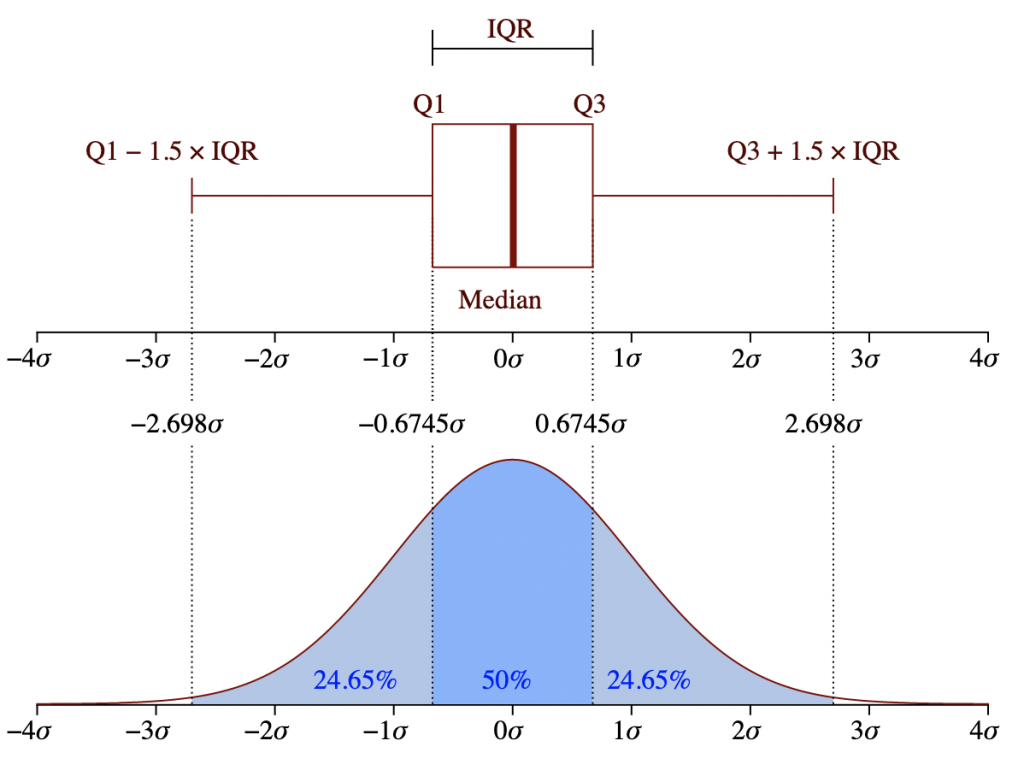
\includegraphics[width=.8\textwidth]{images/IQR.png}
    \caption{Esempio di scarto interquartile in una distribuzione normale \cite{wikipedia:iqr}}
    \label{fig:iqr}
\end{figure}

\subsubsection{Winsorizing (Percentile Capping)}
E' un metodo simile al metodo IQR, in questo caso si utilizzano due percentili. Tutti i valori sotto al minimo valore dell'intervallo vengono sostituiti con il minimo, e tutti i valori sopra il massimo valore dell'intervallo vengono sostituiti con il massimo. In questo lavoro sono stati usati due intervalli ($5^{\circ}$ percentile, $95^{\circ}$ percentile) e ($1^{\circ}$ percentile, $99^{\circ}$ percentile).

\noindent
I due intervalli sono stati denominati Winsorizing 90\% e Winsorizing 98\%:
\begin{itemize}
    \item Winsorizing 90\% indica che il 5\% inferiore dei dati viene sostituito con il $5^{\circ}$ percentile e il 5\% superiore dei dati viene sostituito con il $95^{\circ}$ percentile.
    \item Winsorizing 98\% indica che l' 1\% inferiore dei dati viene sostituito con il $1^{\circ}$ percentile e l' 1\% superiore dei dati viene sostituito con il $99^{\circ}$ percentile.
\end{itemize}

\subsubsection{Metodo Scelto}
Un grafico abbastanza semplice e veloce per visualizzare gli outlier è il boxplot. \'{E} stato confrontato ogni variabile del dataset con i valori assunti dopo l'applicazione dei metodi di rimozione degli outlier (IQR, Winsorizing 90\% e Winsorizing 98\%), attraverso dei boxplot. Sopra a ogni boxplot sono stati riportati i valori divisi per qualità.

\noindent
Il metodo Winsorizing rileva un intervallo di outlier più piccolo e variabile rispetto all'IQR. Inoltre nei casi di distribuzione con distorsione laterale accumula troppi valori agli estremi, alterando così la distribuzione. Con il metodo Winsorizing 98\% si risulta avere una distribuzione più smussata agli estremi. Il metodo IQR, sostituendo con la mediana non altera molto la distribuzione.
Per decidere il metodo più efficace da usare sono stati confrontati dati dopo l'applicazione di ogni metodo attraverso dei Q-Q plot.

\noindent
I Q-Q (quantile-quantile) plot sono dei grafici utili per capire se due insiemi di dati hanno la stessa distribuzione. Vengono rappresentati i punti in un piano cartesiano attraverso una coppia di quantili. Inoltre viene tracciata una retta a 45° in modo da evidenziare i punti più vicini alla retta. Due insiemi di dati hanno una distribuzione simile se i punti cadono approssimatamene sulla linea di riferimento.
Analizzando i grafici si è visto che il metodo IQR ha valori più vicini alla retta, quindi si è scelto di utilizzare questo.

\noindent
Nelle seguenti tabelle sono stati riportati le varie statistiche descrittive delle variabili prima e dopo la rimozione degli outlier con il metodo scelto.

\begin{table}[H]
\centering
\resizebox{\linewidth}{!}{
\begin{tabular}[t]{lrrrrrrrr}
\toprule
  & vars & mean & sd & median & min & max & skew & kurtosis\\
\midrule
\cellcolor{gray!6}{fixed.acidity} & \cellcolor{gray!6}{1} & \cellcolor{gray!6}{8.34} & \cellcolor{gray!6}{1.78} & \cellcolor{gray!6}{7.90} & \cellcolor{gray!6}{4.70} & \cellcolor{gray!6}{15.90} & \cellcolor{gray!6}{0.98} & \cellcolor{gray!6}{1.13}\\
volatile.acidity & 2 & 0.53 & 0.18 & 0.52 & 0.12 & 1.58 & 0.71 & 1.46\\
\cellcolor{gray!6}{citric.acid} & \cellcolor{gray!6}{3} & \cellcolor{gray!6}{0.27} & \cellcolor{gray!6}{0.19} & \cellcolor{gray!6}{0.26} & \cellcolor{gray!6}{0.00} & \cellcolor{gray!6}{1.00} & \cellcolor{gray!6}{0.32} & \cellcolor{gray!6}{-0.79}\\
residual.sugar & 4 & 2.53 & 1.40 & 2.20 & 0.90 & 15.40 & 4.47 & 27.53\\
\cellcolor{gray!6}{chlorides} & \cellcolor{gray!6}{5} & \cellcolor{gray!6}{0.09} & \cellcolor{gray!6}{0.05} & \cellcolor{gray!6}{0.08} & \cellcolor{gray!6}{0.01} & \cellcolor{gray!6}{0.61} & \cellcolor{gray!6}{5.89} & \cellcolor{gray!6}{45.36}\\
\addlinespace
free.sulfur.dioxide & 6 & 15.79 & 10.58 & 13.00 & 1.00 & 72.00 & 1.29 & 2.19\\
\cellcolor{gray!6}{total.sulfur.dioxide} & \cellcolor{gray!6}{7} & \cellcolor{gray!6}{45.23} & \cellcolor{gray!6}{31.87} & \cellcolor{gray!6}{37.00} & \cellcolor{gray!6}{6.00} & \cellcolor{gray!6}{278.00} & \cellcolor{gray!6}{1.41} & \cellcolor{gray!6}{2.87}\\
density & 8 & 1.00 & 0.00 & 1.00 & 0.99 & 1.00 & 0.05 & 0.90\\
\cellcolor{gray!6}{pH} & \cellcolor{gray!6}{9} & \cellcolor{gray!6}{3.31} & \cellcolor{gray!6}{0.15} & \cellcolor{gray!6}{3.31} & \cellcolor{gray!6}{2.74} & \cellcolor{gray!6}{4.01} & \cellcolor{gray!6}{0.11} & \cellcolor{gray!6}{0.62}\\
sulphates & 10 & 0.66 & 0.17 & 0.62 & 0.33 & 2.00 & 2.57 & 13.02\\
\addlinespace
\cellcolor{gray!6}{alcohol} & \cellcolor{gray!6}{11} & \cellcolor{gray!6}{10.45} & \cellcolor{gray!6}{1.07} & \cellcolor{gray!6}{10.20} & \cellcolor{gray!6}{8.40} & \cellcolor{gray!6}{14.90} & \cellcolor{gray!6}{0.84} & \cellcolor{gray!6}{0.13}\\
\bottomrule
\end{tabular}}
\caption{Prima della rimozione}
\end{table}


\begin{table}
\centering
\resizebox{\linewidth}{!}{
\begin{tabular}[t]{lrrrrrrrr}
\toprule
  & vars & mean & sd & median & min & max & skew & kurtosis\\
\midrule
\cellcolor{gray!6}{fixed.acidity} & \cellcolor{gray!6}{1} & \cellcolor{gray!6}{6.83} & \cellcolor{gray!6}{0.77} & \cellcolor{gray!6}{6.80} & \cellcolor{gray!6}{4.70} & \cellcolor{gray!6}{9.00} & \cellcolor{gray!6}{0.22} & \cellcolor{gray!6}{0.02}\\
volatile.acidity & 2 & 0.27 & 0.08 & 0.26 & 0.08 & 0.48 & 0.41 & -0.23\\
\cellcolor{gray!6}{citric.acid} & \cellcolor{gray!6}{3} & \cellcolor{gray!6}{0.32} & \cellcolor{gray!6}{0.09} & \cellcolor{gray!6}{0.31} & \cellcolor{gray!6}{0.10} & \cellcolor{gray!6}{0.57} & \cellcolor{gray!6}{0.41} & \cellcolor{gray!6}{-0.02}\\
residual.sugar & 4 & 6.39 & 4.96 & 5.20 & 0.60 & 22.00 & 0.73 & -0.52\\
\cellcolor{gray!6}{chlorides} & \cellcolor{gray!6}{5} & \cellcolor{gray!6}{0.04} & \cellcolor{gray!6}{0.01} & \cellcolor{gray!6}{0.04} & \cellcolor{gray!6}{0.02} & \cellcolor{gray!6}{0.07} & \cellcolor{gray!6}{0.10} & \cellcolor{gray!6}{-0.25}\\
\addlinespace
free.sulfur.dioxide & 6 & 34.53 & 15.28 & 33.00 & 2.00 & 78.00 & 0.32 & -0.45\\
\cellcolor{gray!6}{total.sulfur.dioxide} & \cellcolor{gray!6}{7} & \cellcolor{gray!6}{138.24} & \cellcolor{gray!6}{41.26} & \cellcolor{gray!6}{135.00} & \cellcolor{gray!6}{21.00} & \cellcolor{gray!6}{256.00} & \cellcolor{gray!6}{0.23} & \cellcolor{gray!6}{-0.33}\\
density & 8 & 0.99 & 0.00 & 0.99 & 0.99 & 1.00 & 0.23 & -0.78\\
\cellcolor{gray!6}{pH} & \cellcolor{gray!6}{9} & \cellcolor{gray!6}{3.18} & \cellcolor{gray!6}{0.14} & \cellcolor{gray!6}{3.17} & \cellcolor{gray!6}{2.79} & \cellcolor{gray!6}{3.57} & \cellcolor{gray!6}{0.22} & \cellcolor{gray!6}{-0.18}\\
sulphates & 10 & 0.48 & 0.10 & 0.47 & 0.23 & 0.76 & 0.48 & -0.08\\
\addlinespace
\cellcolor{gray!6}{alcohol} & \cellcolor{gray!6}{11} & \cellcolor{gray!6}{10.52} & \cellcolor{gray!6}{1.24} & \cellcolor{gray!6}{10.40} & \cellcolor{gray!6}{8.00} & \cellcolor{gray!6}{14.20} & \cellcolor{gray!6}{0.49} & \cellcolor{gray!6}{-0.69}\\
\bottomrule
\end{tabular}}
\end{table}


\subsection{Grafici}

\begin{figure}[H]
    \centering

    \subfloat[]{%
        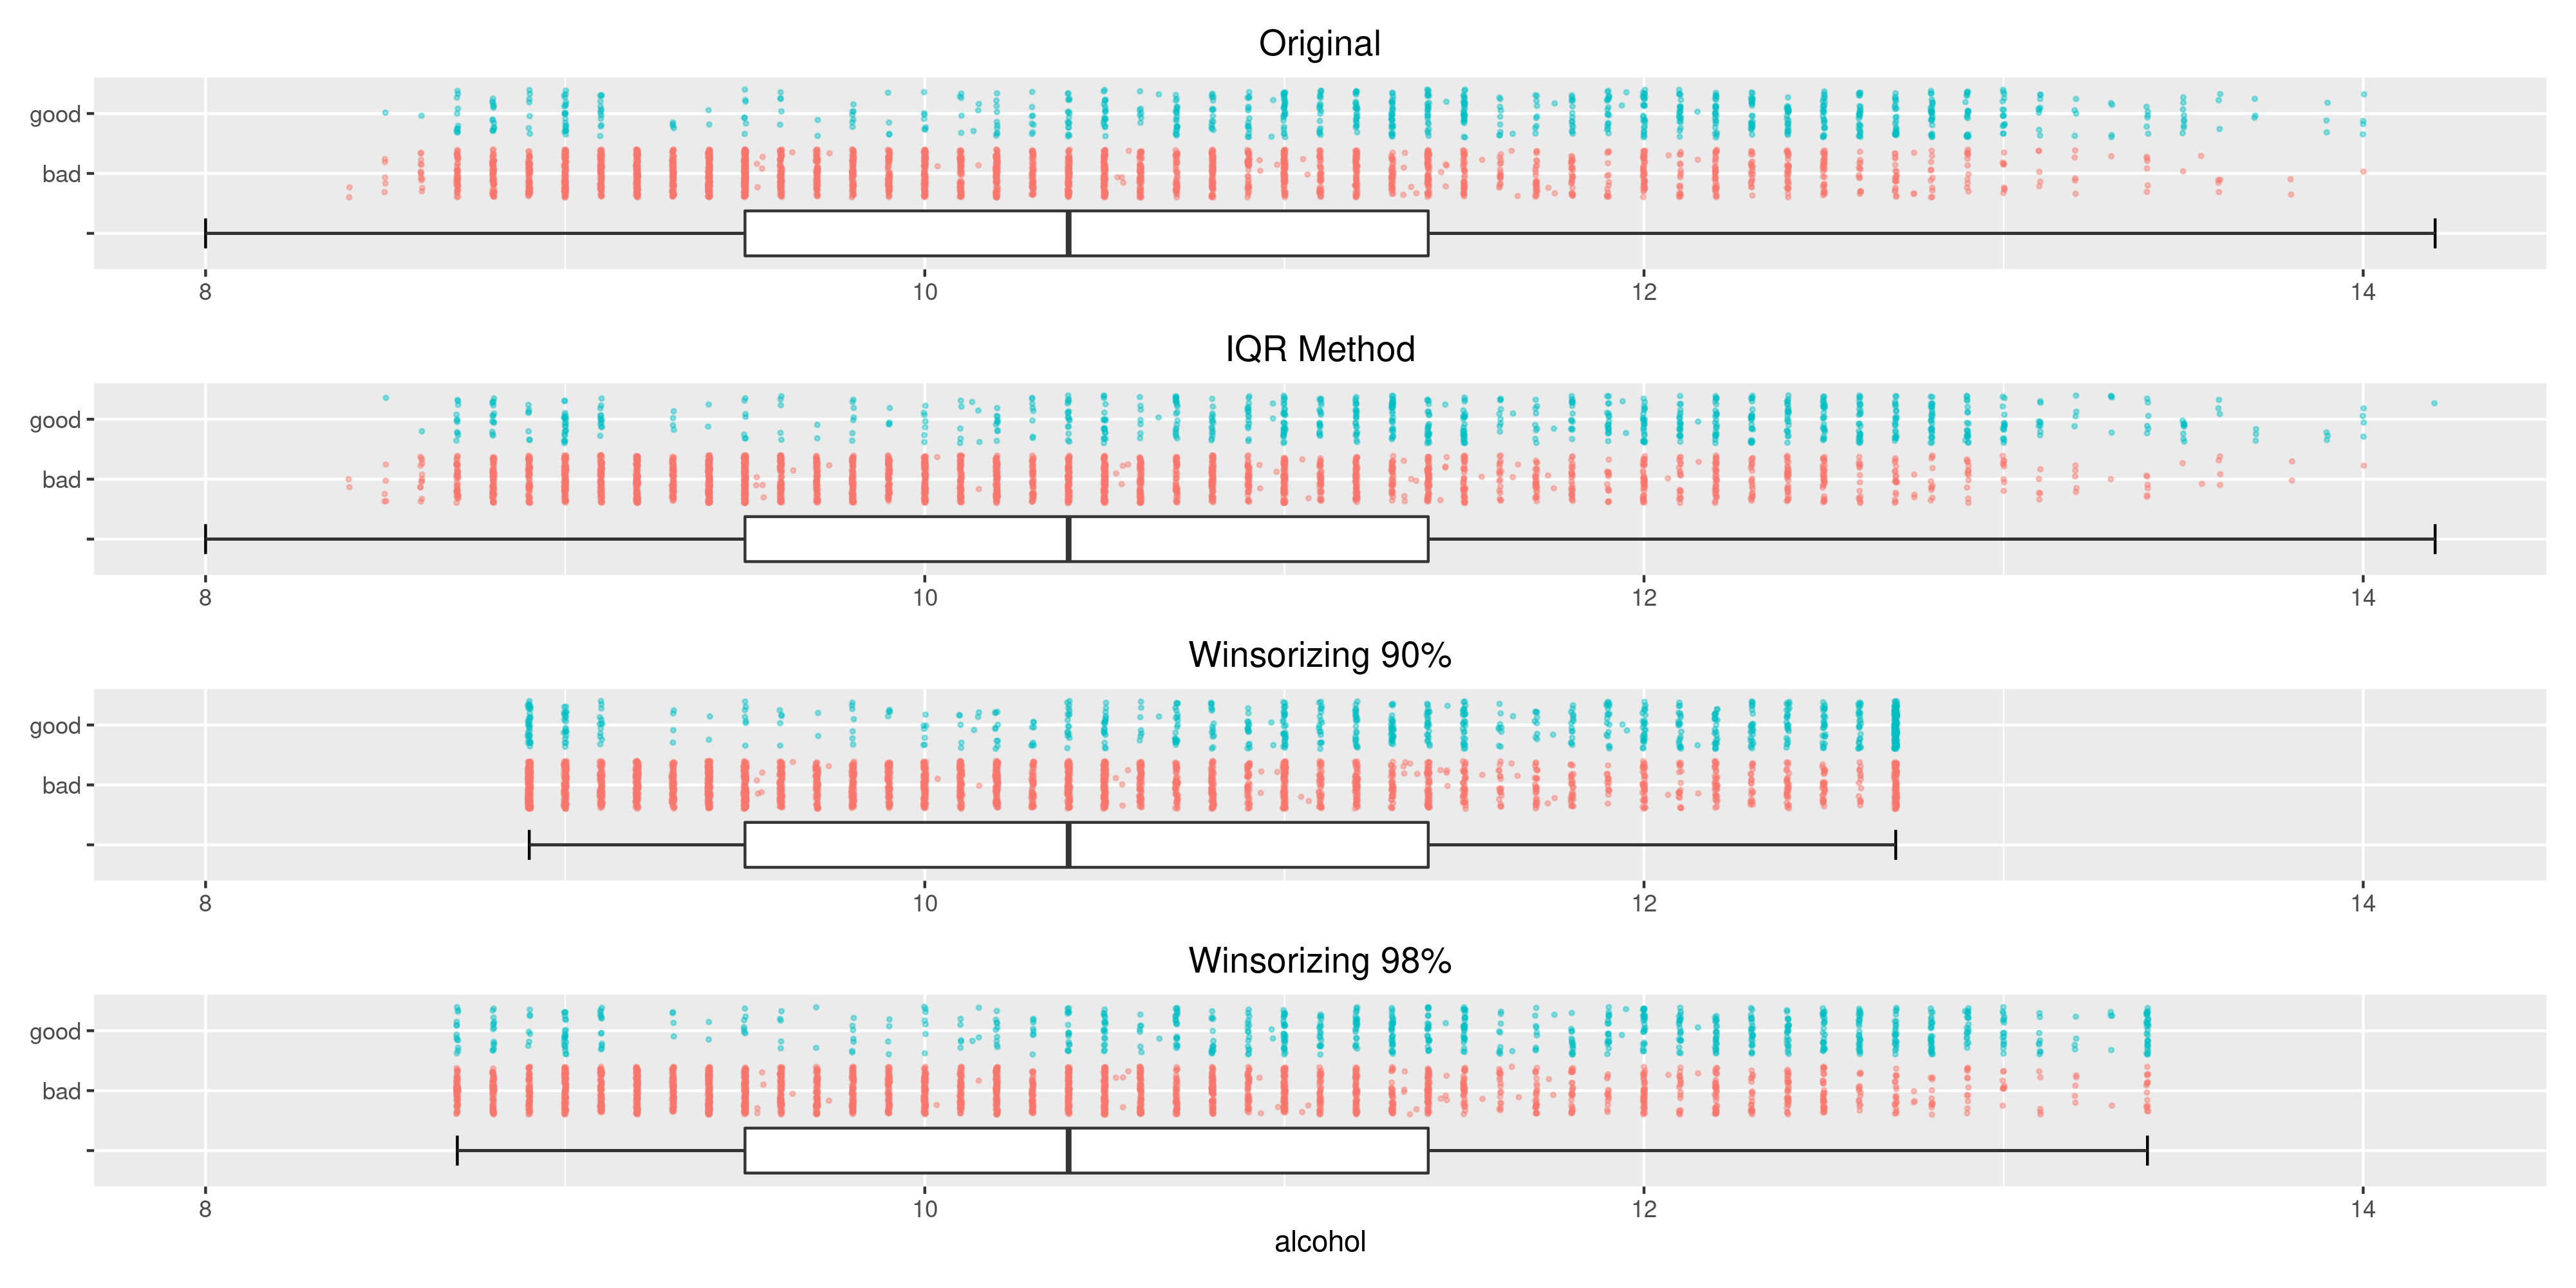
\includegraphics[width=0.99\textwidth]{images/outliers/alcohol_boxplot.png}
    }

    \subfloat[]{%
        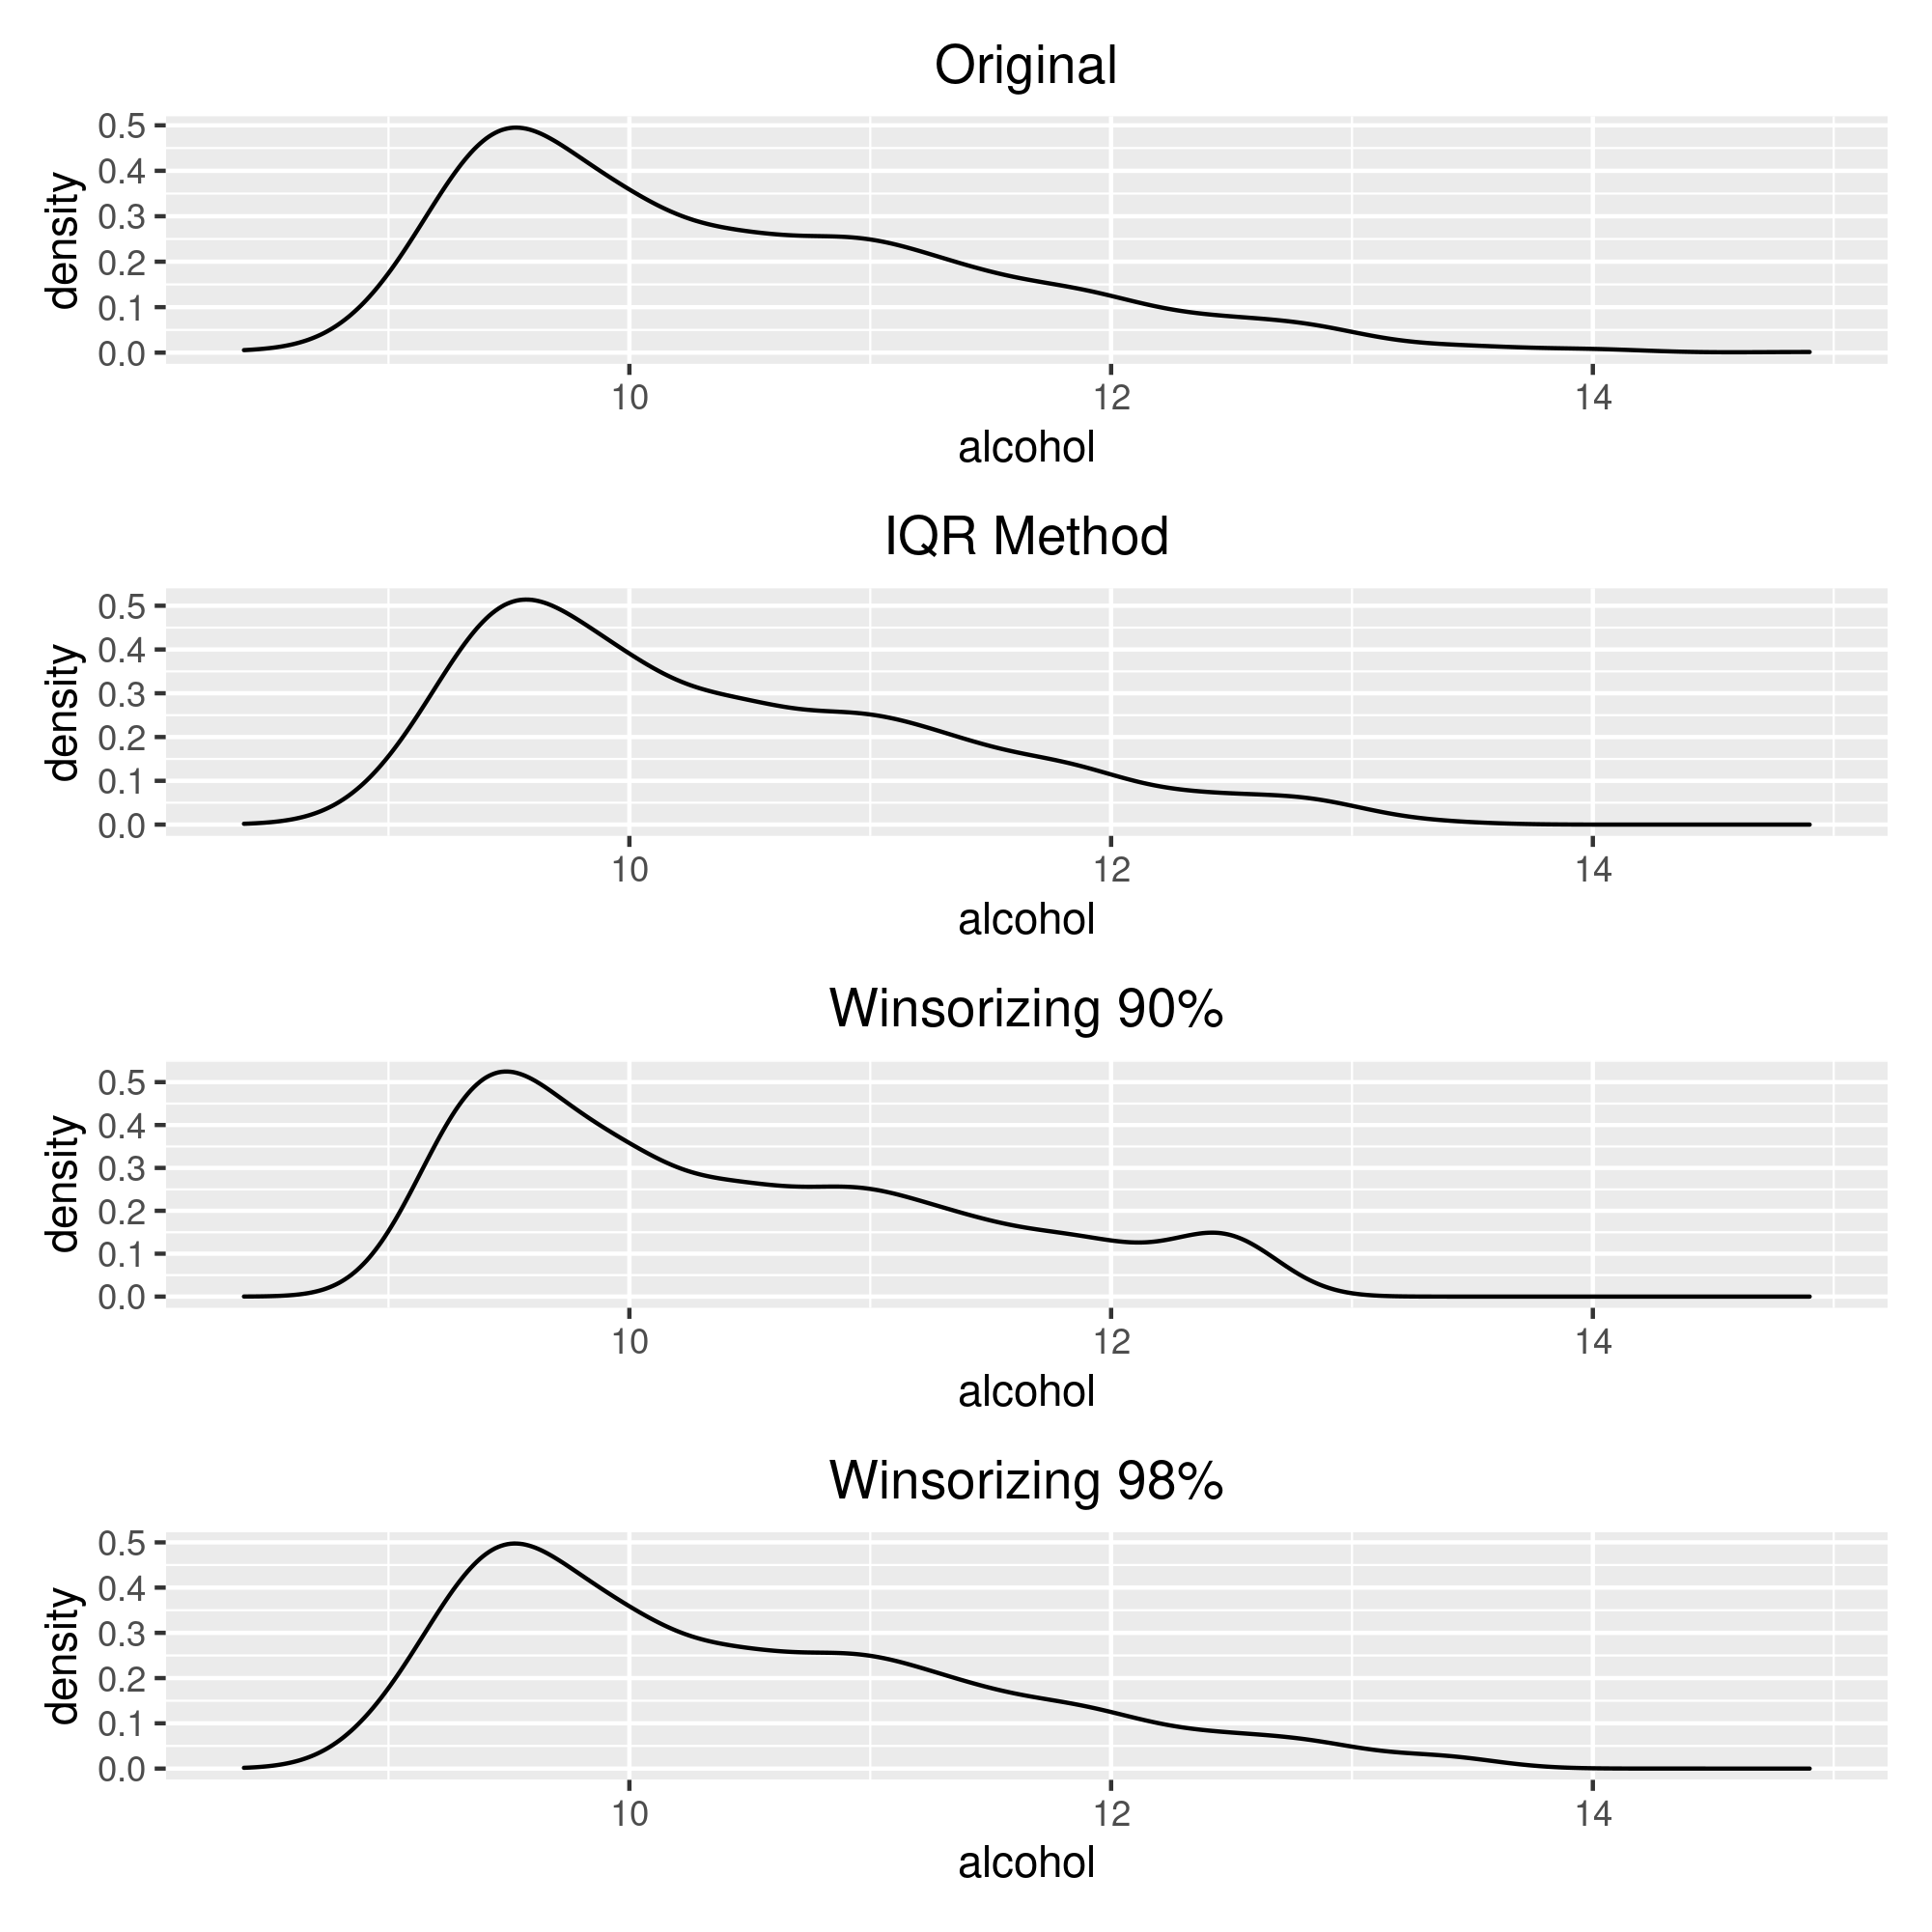
\includegraphics[width=0.45\textwidth]{images/outliers/alcohol_distribution.png}
    }\qquad
    \subfloat[]{%
        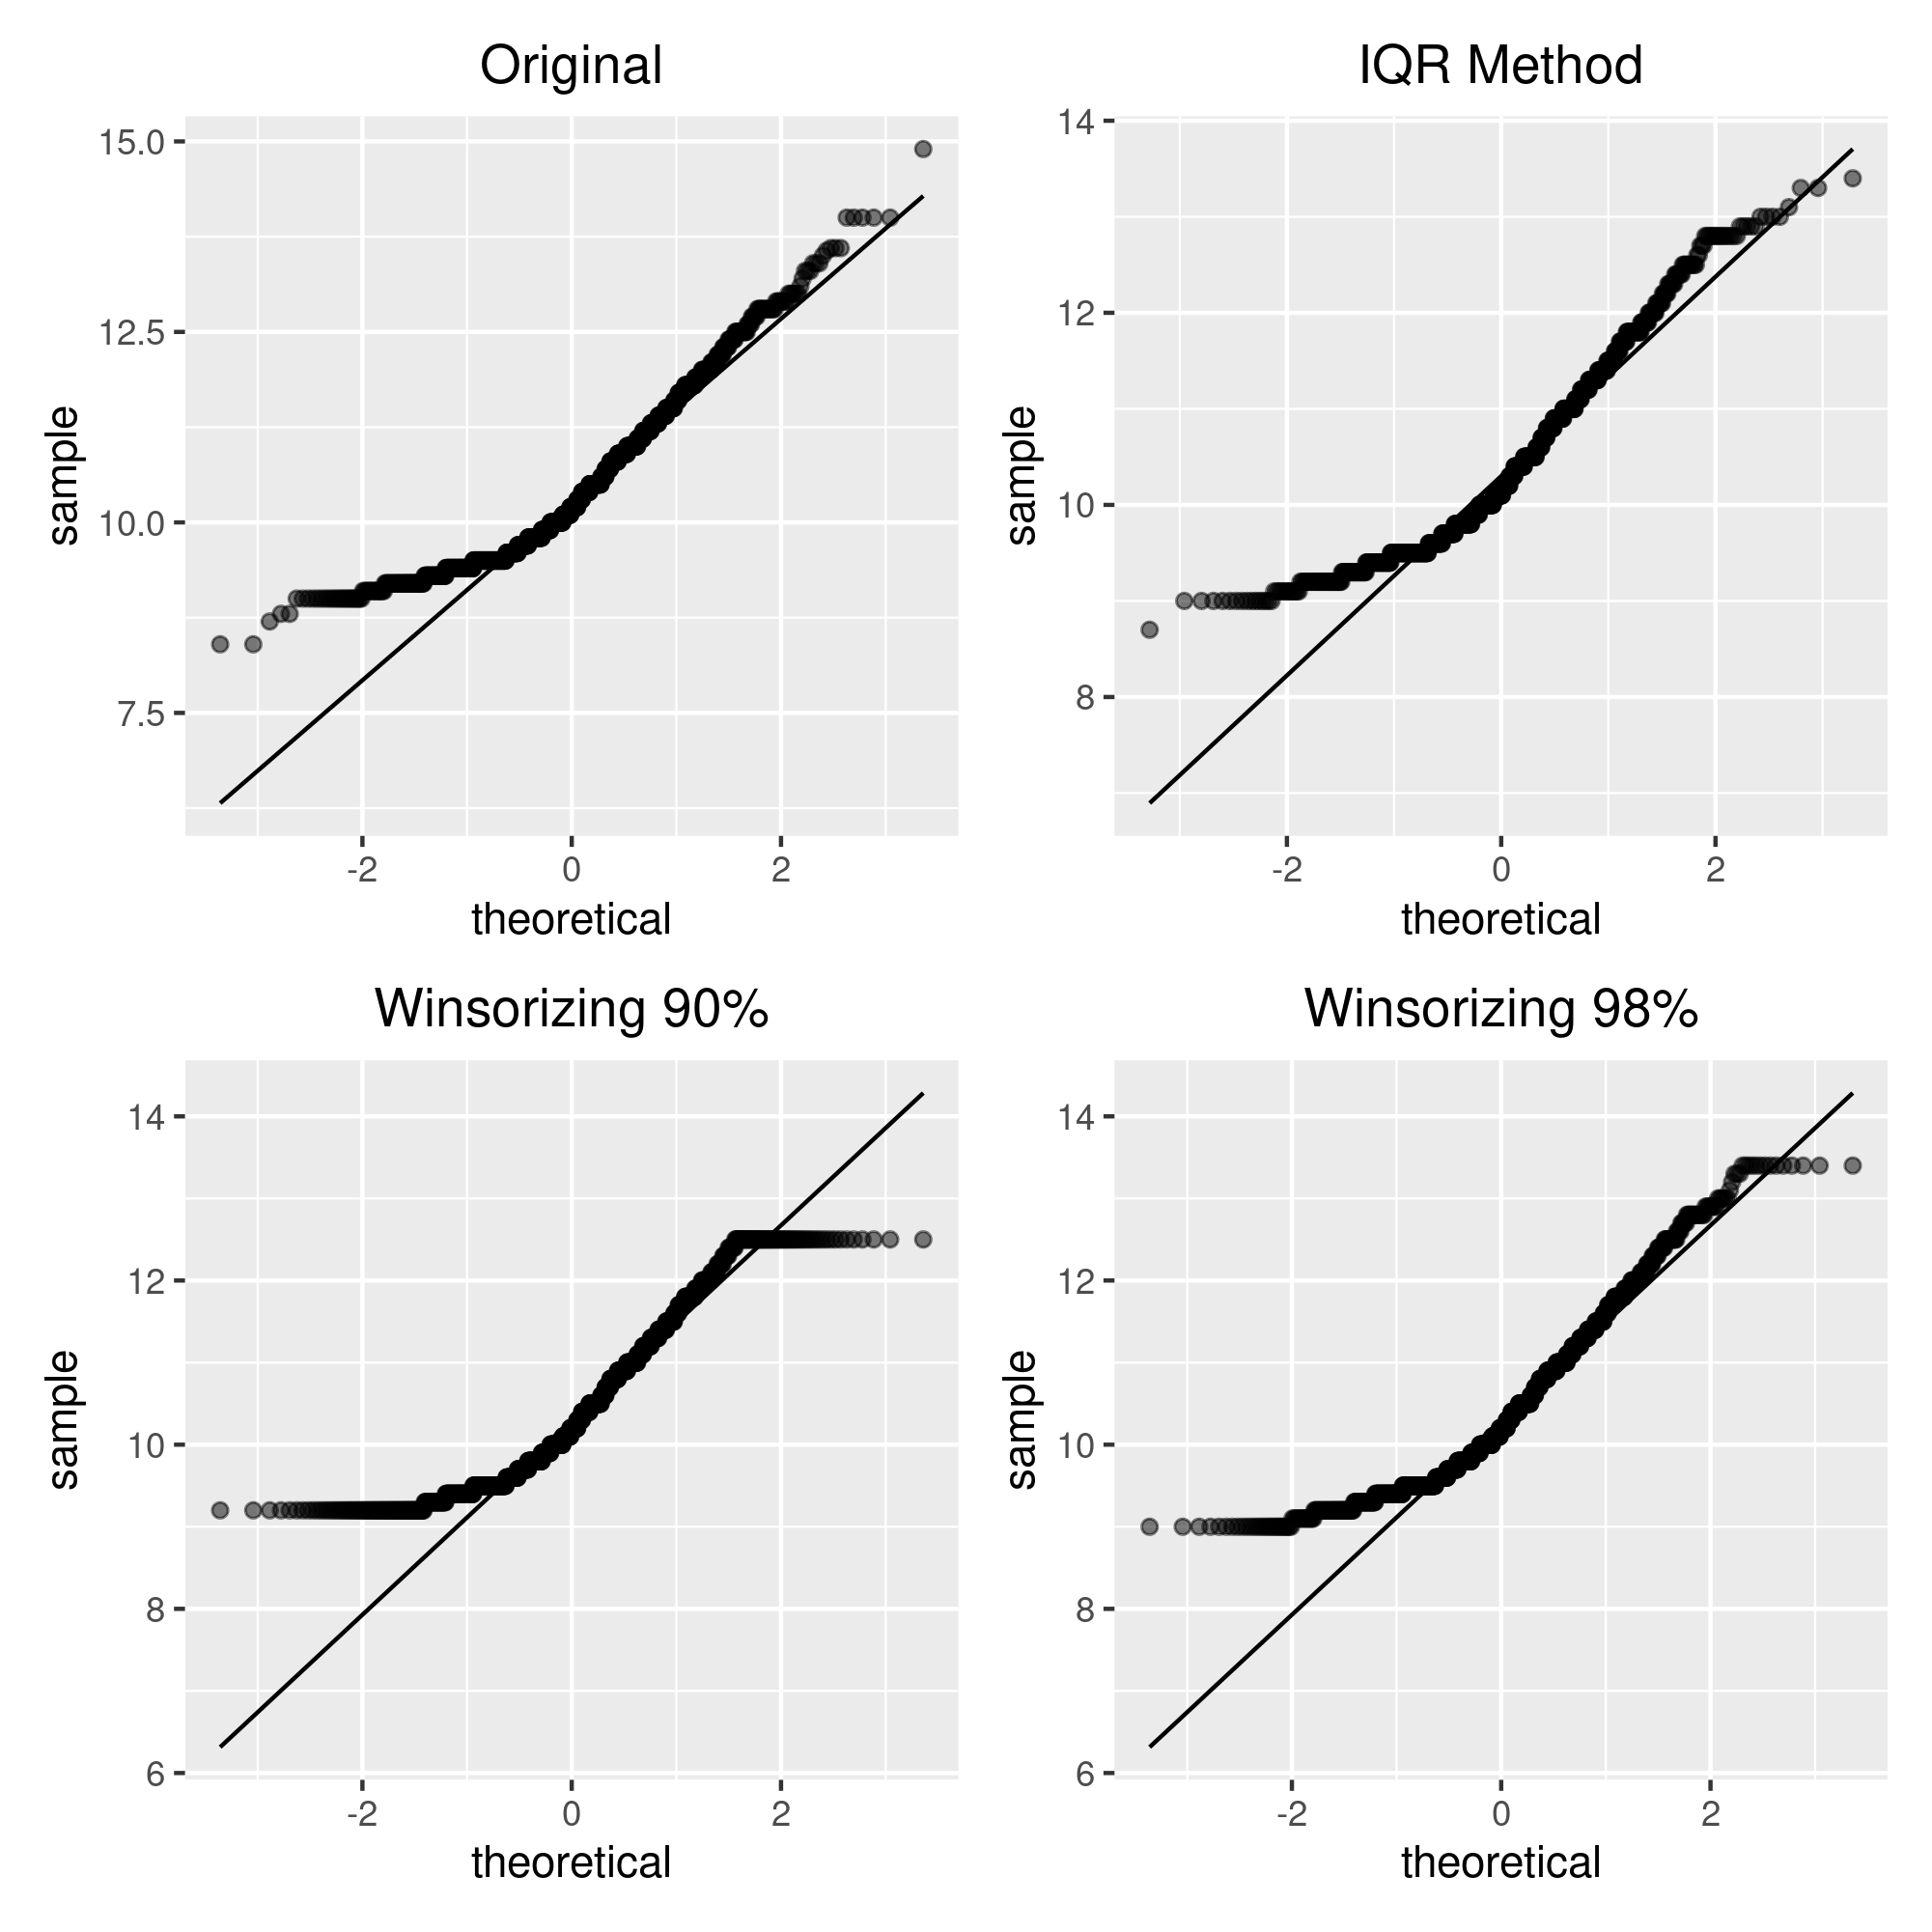
\includegraphics[width=0.45\textwidth]{images/outliers/alcohol_qqplot.png}
    }

    \label{fig:alcohol}
    \caption{Commento}
\end{figure}

\begin{figure}[H]
    \centering

    \subfloat[]{%
        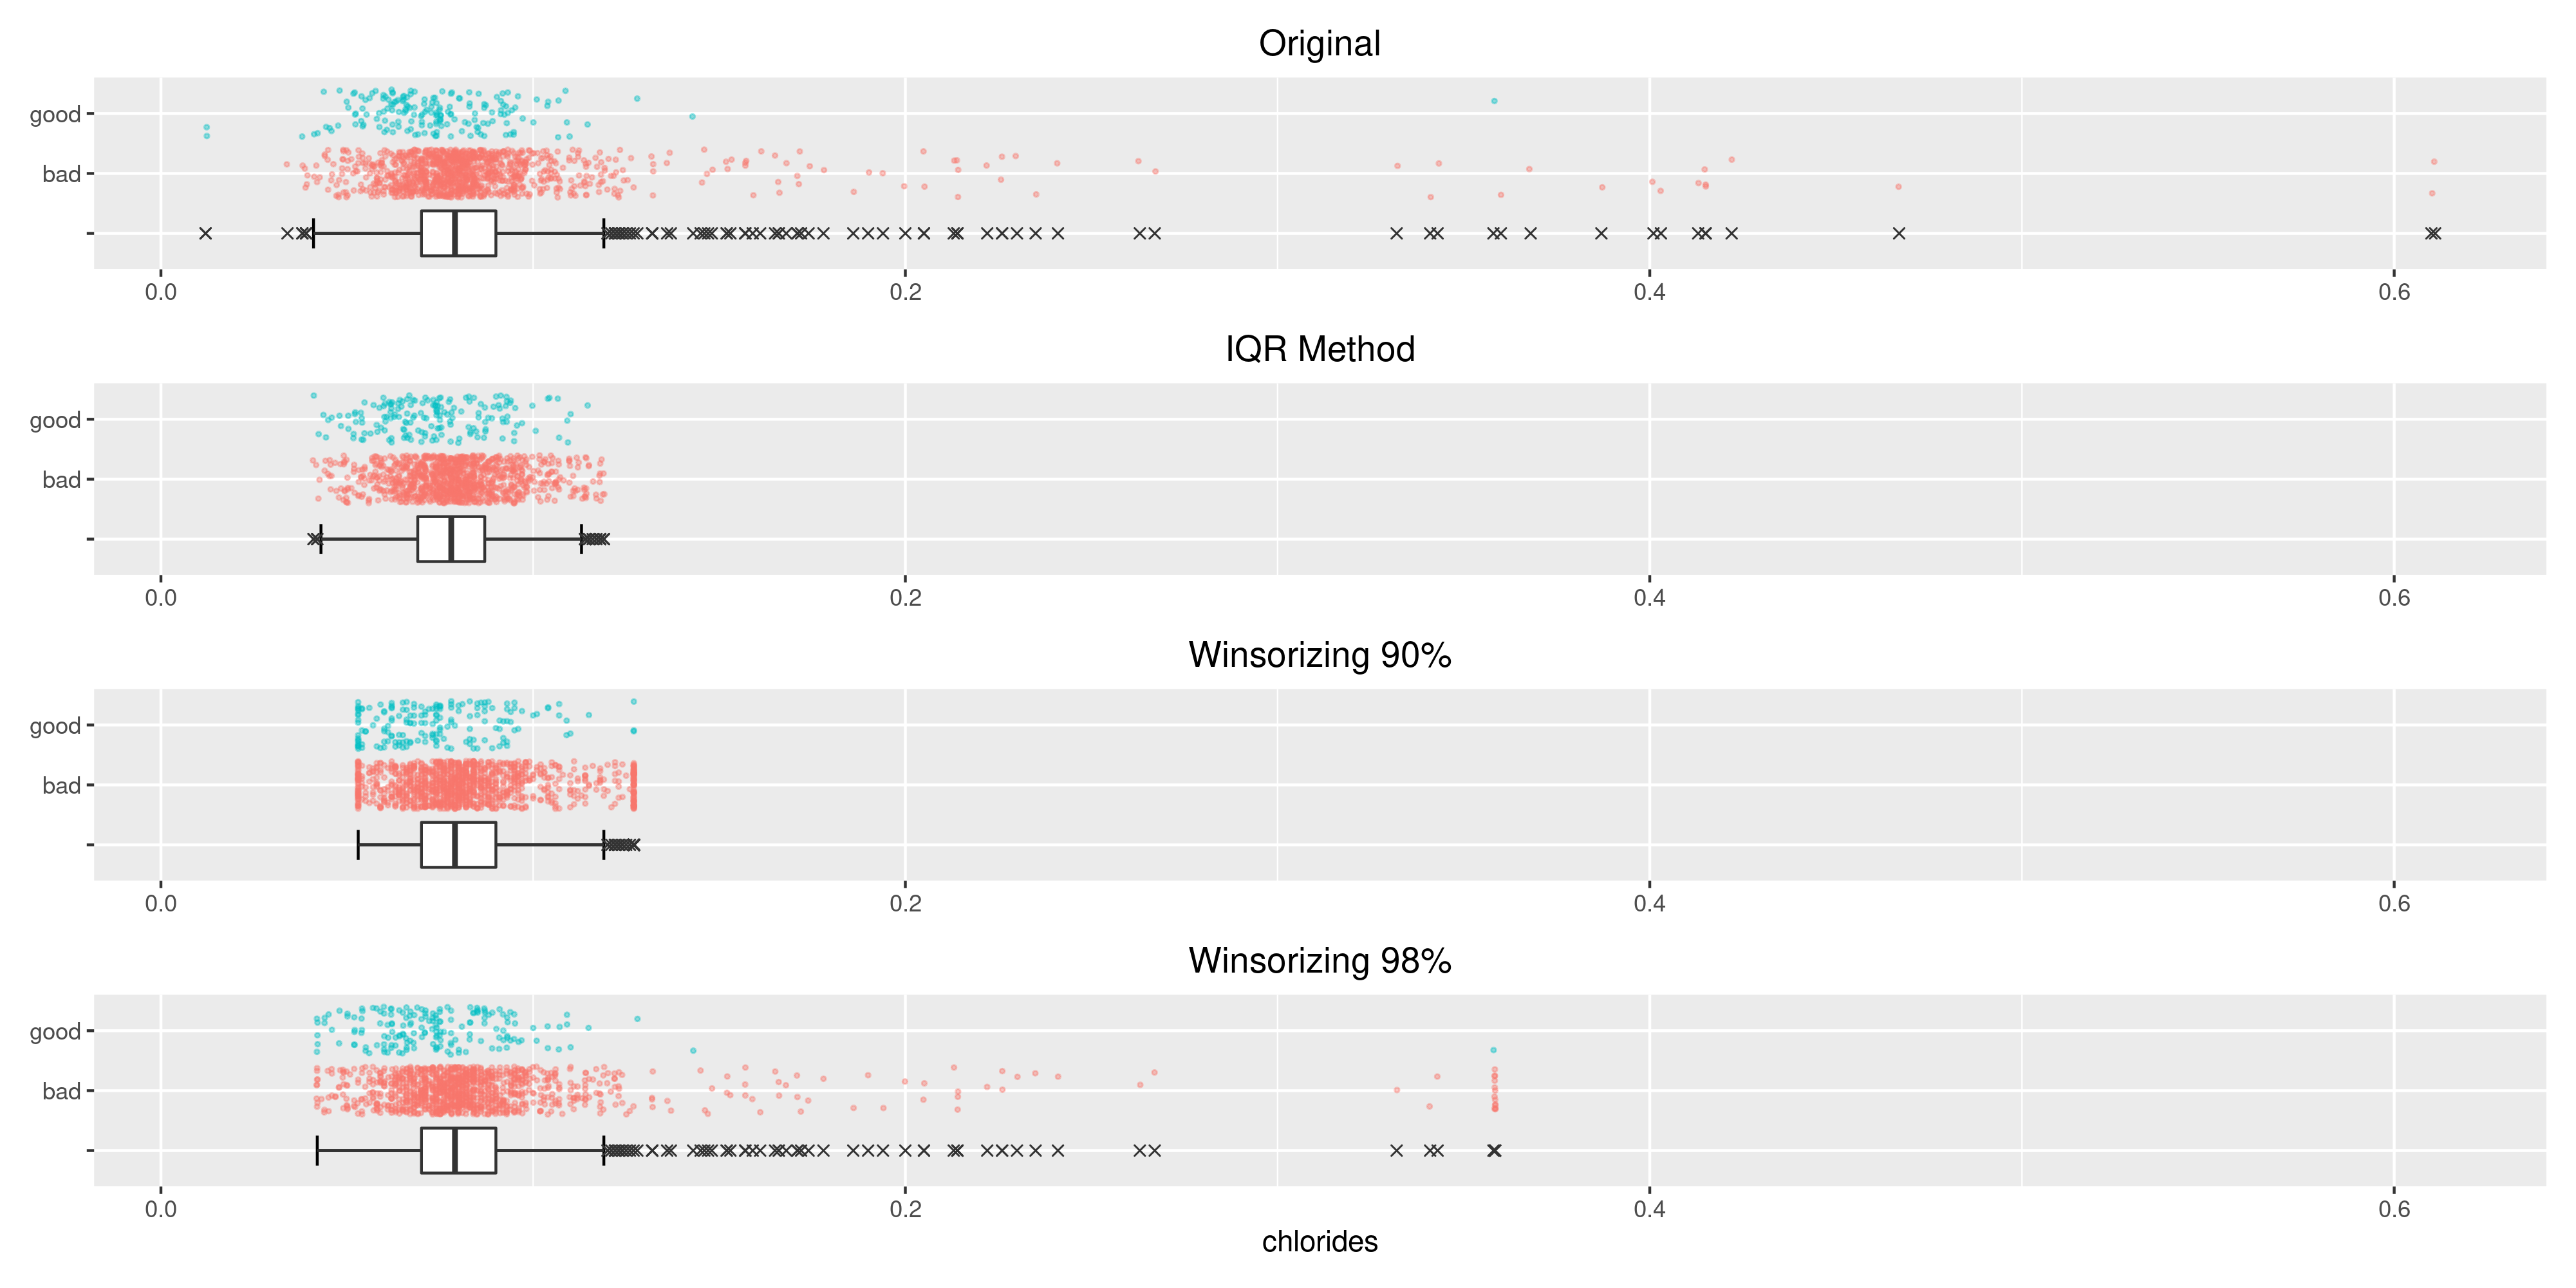
\includegraphics[width=0.99\textwidth]{images/outliers/chlorides_boxplot.png}
    }

    \subfloat[]{%
        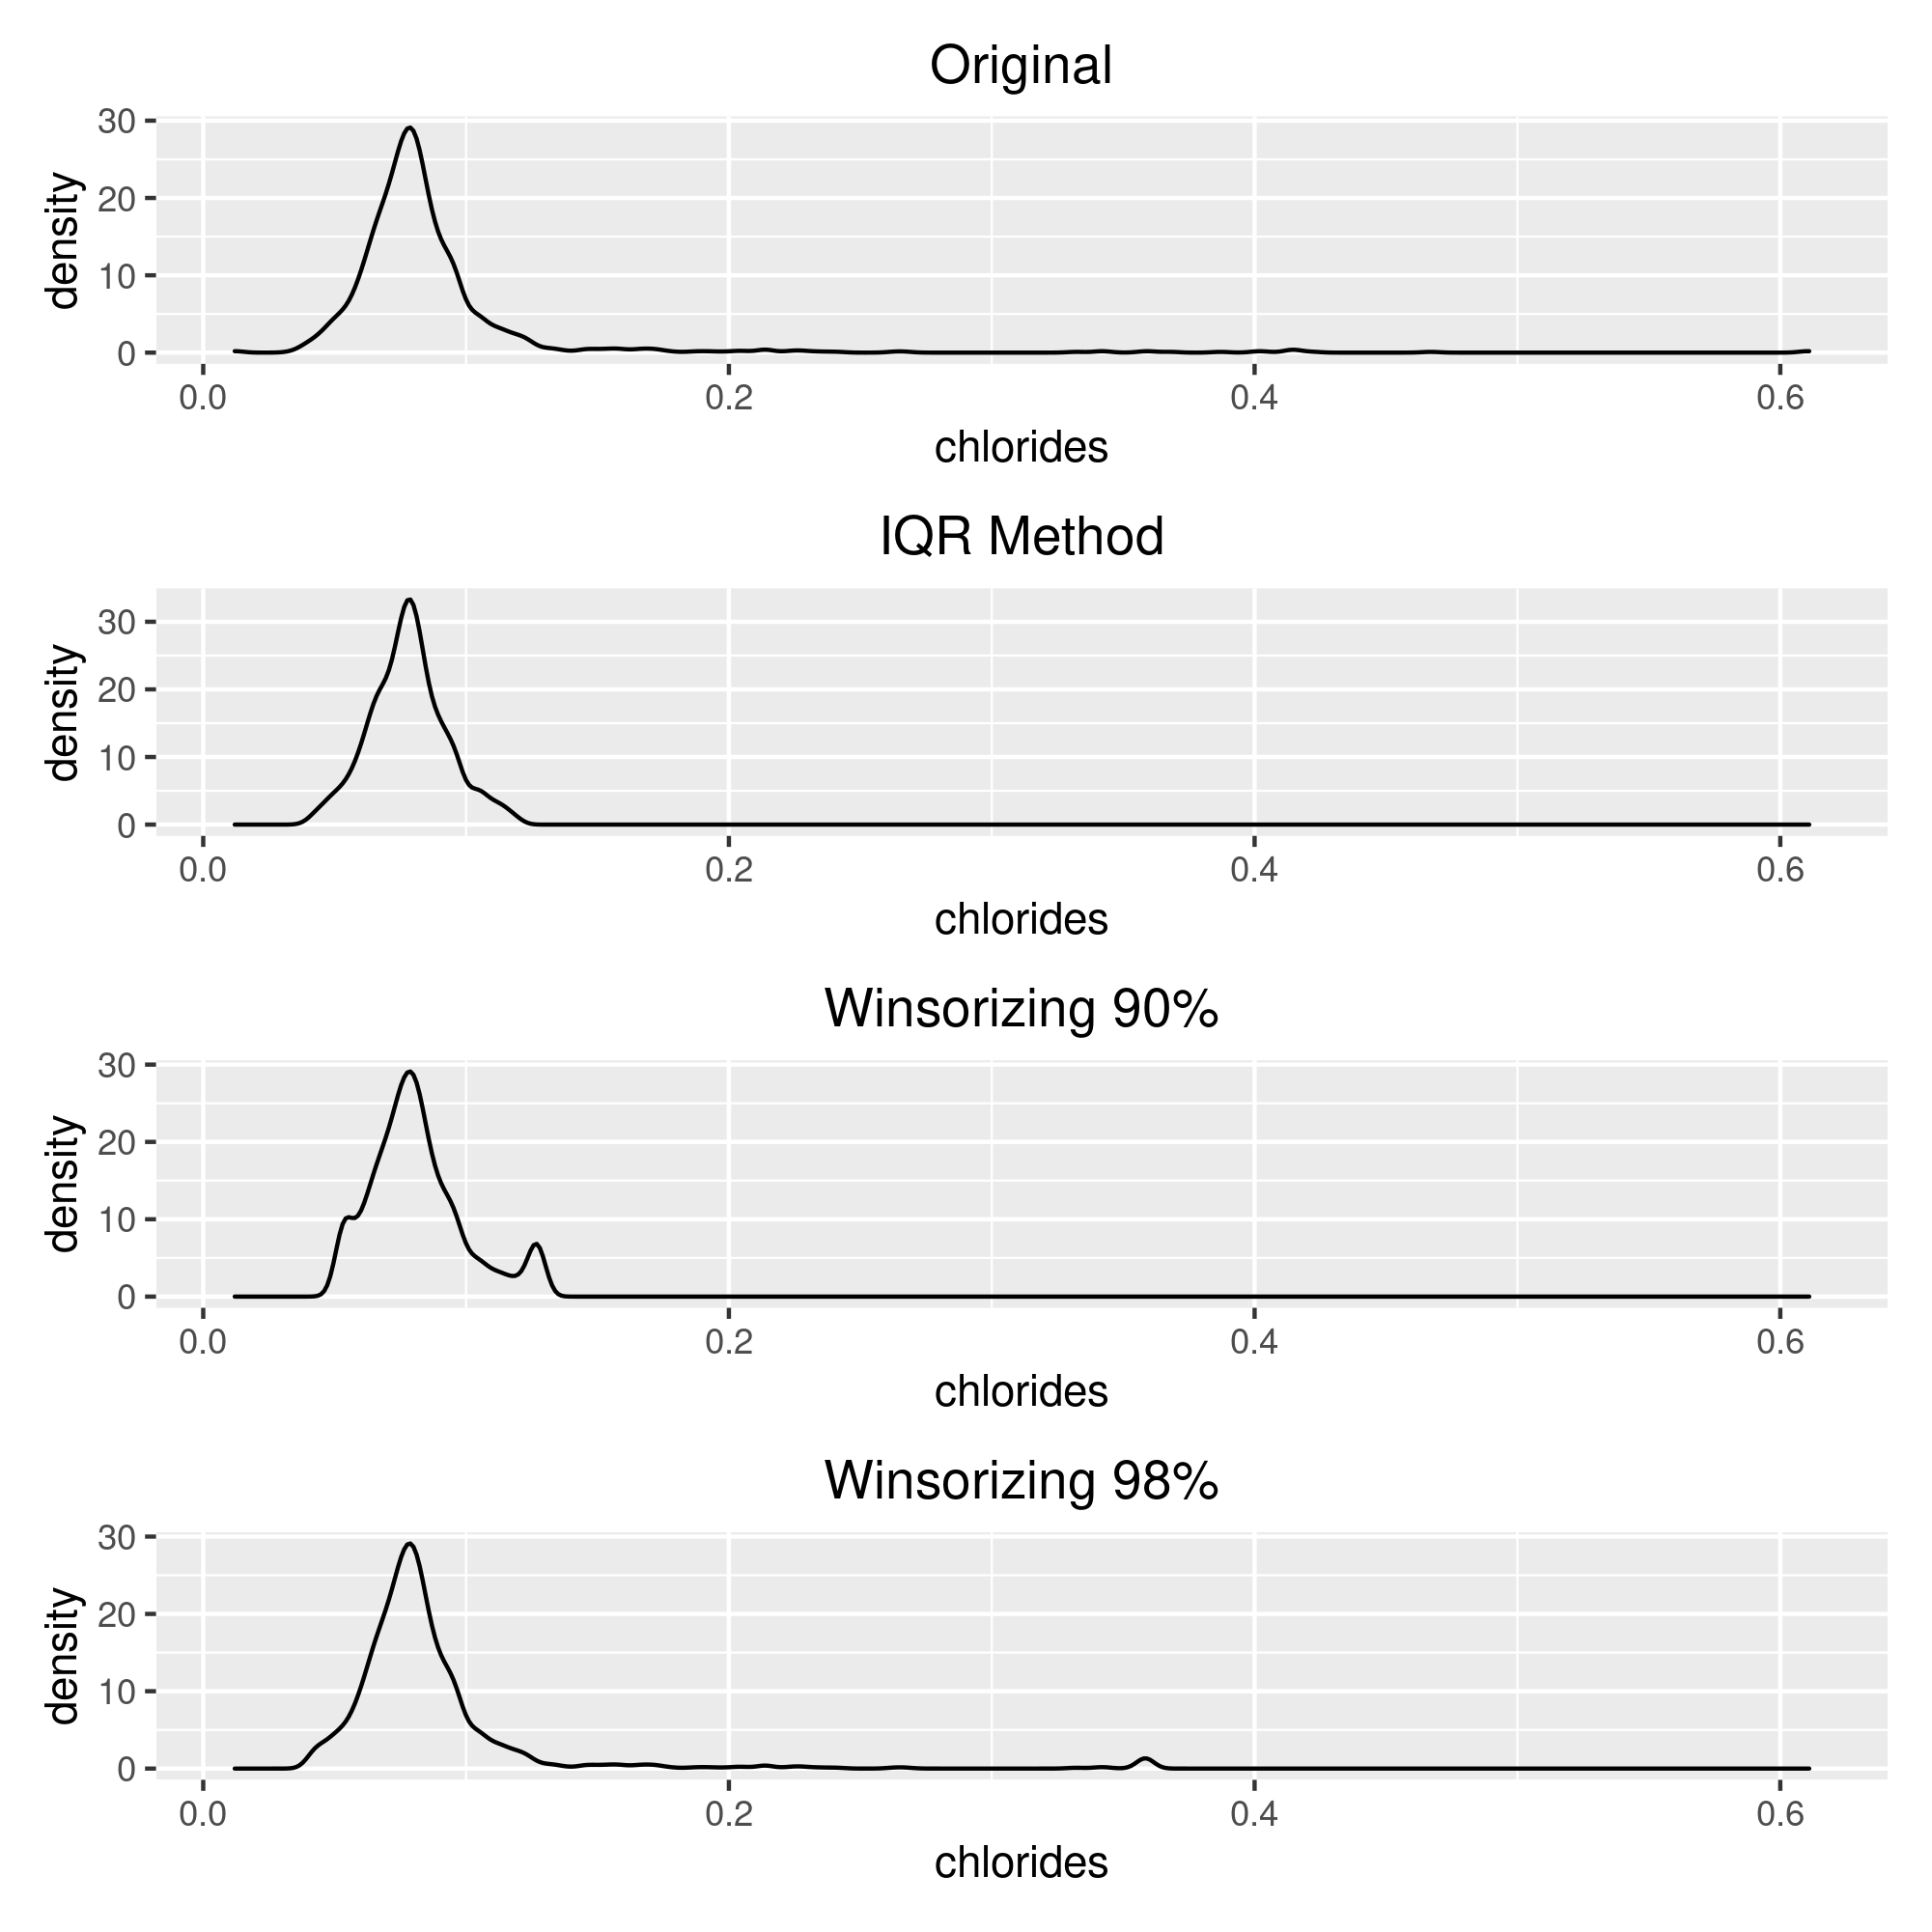
\includegraphics[width=0.45\textwidth]{images/outliers/chlorides_distribution.png}
    }\qquad
    \subfloat[]{%
        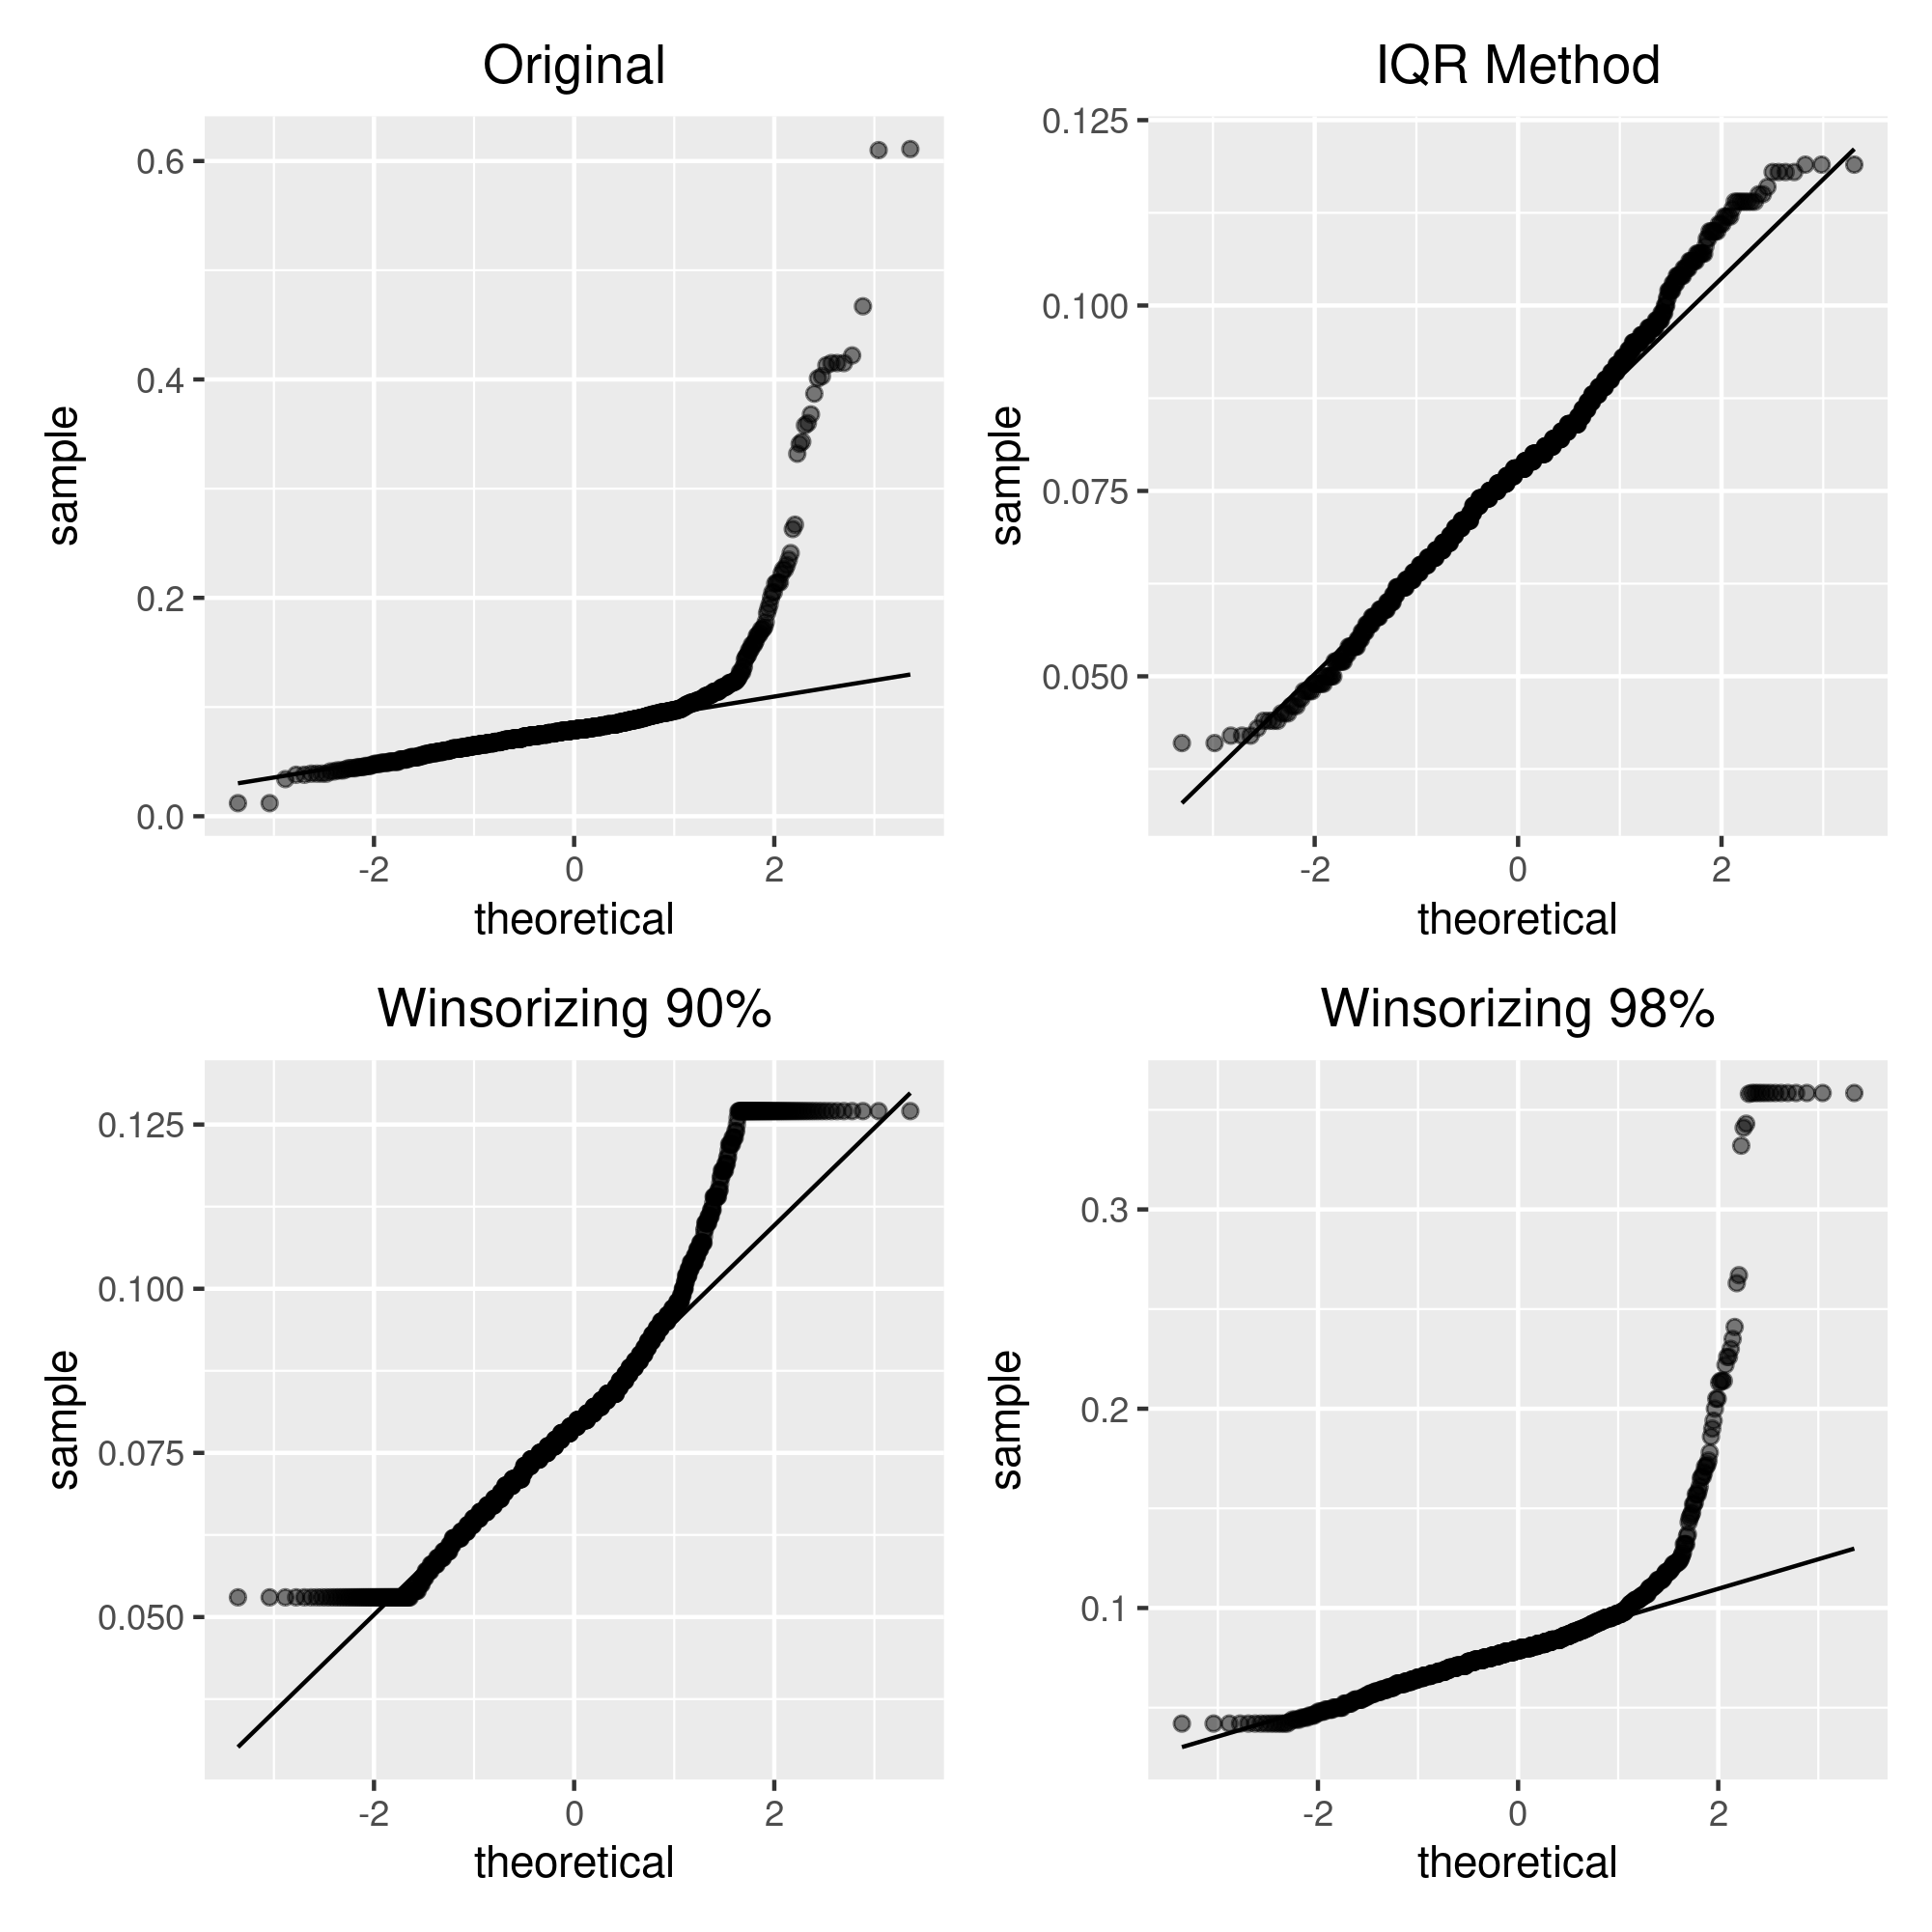
\includegraphics[width=0.45\textwidth]{images/outliers/chlorides_qqplot.png}
    }

    \label{fig:chlorides}
    \caption{Commento}
\end{figure}

\begin{figure}[H]
    \centering

    \subfloat[]{%
        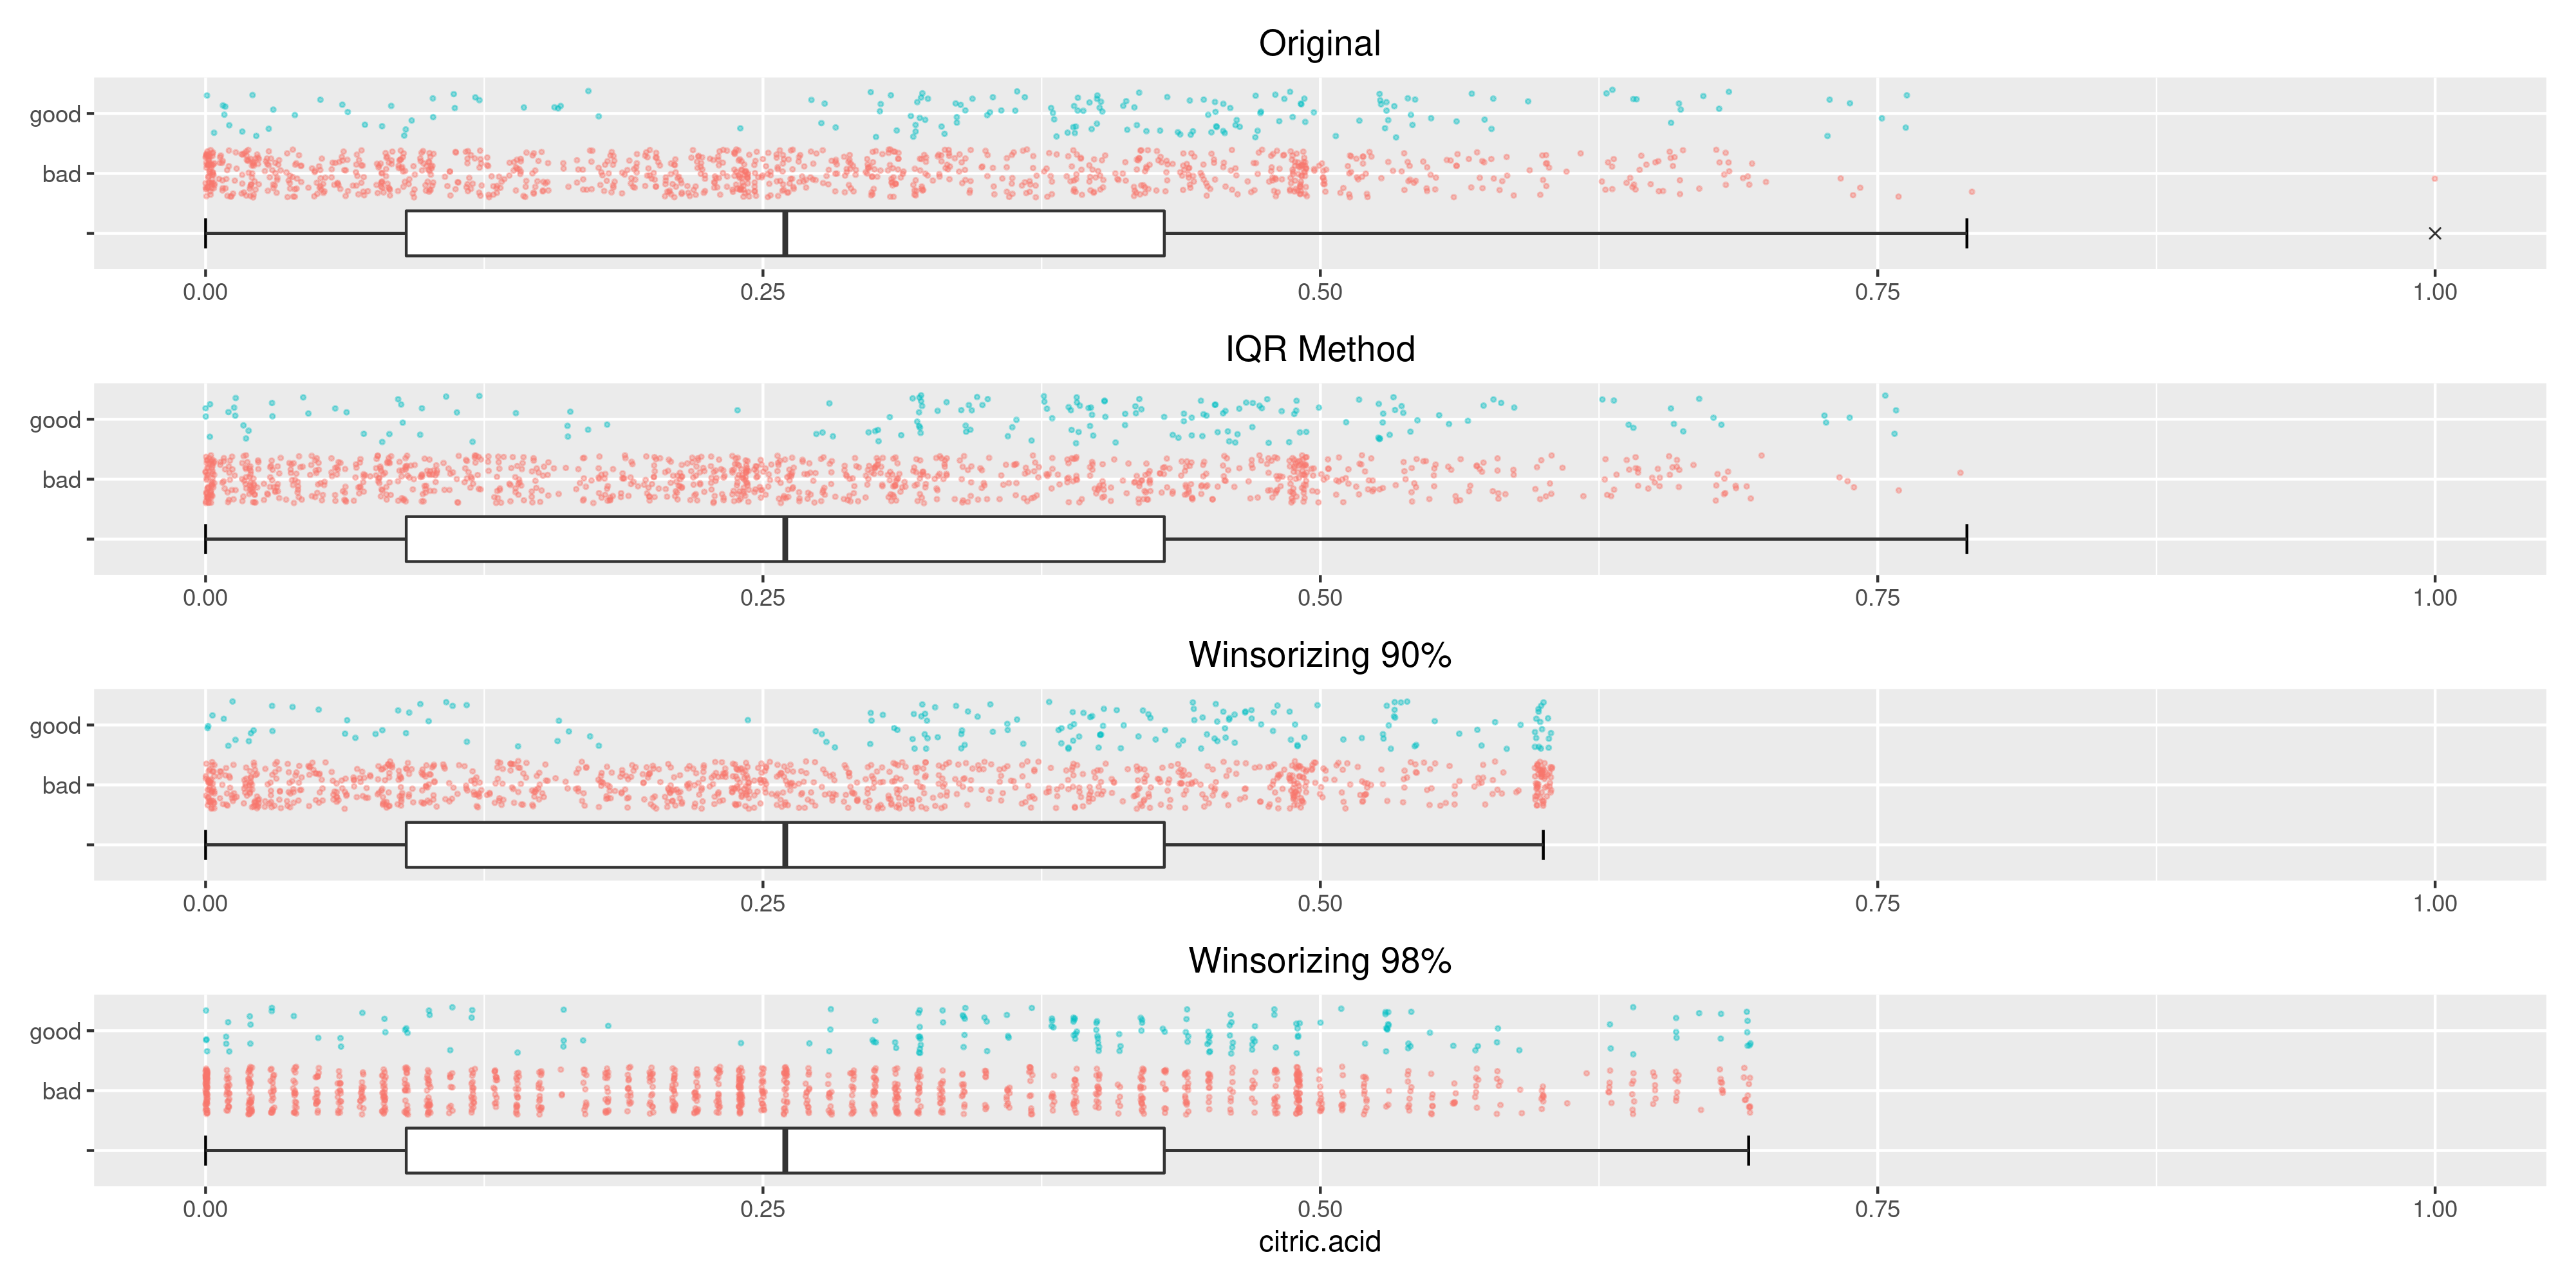
\includegraphics[width=0.99\textwidth]{images/outliers/citric.acid_boxplot.png}
    }

    \subfloat[]{%
        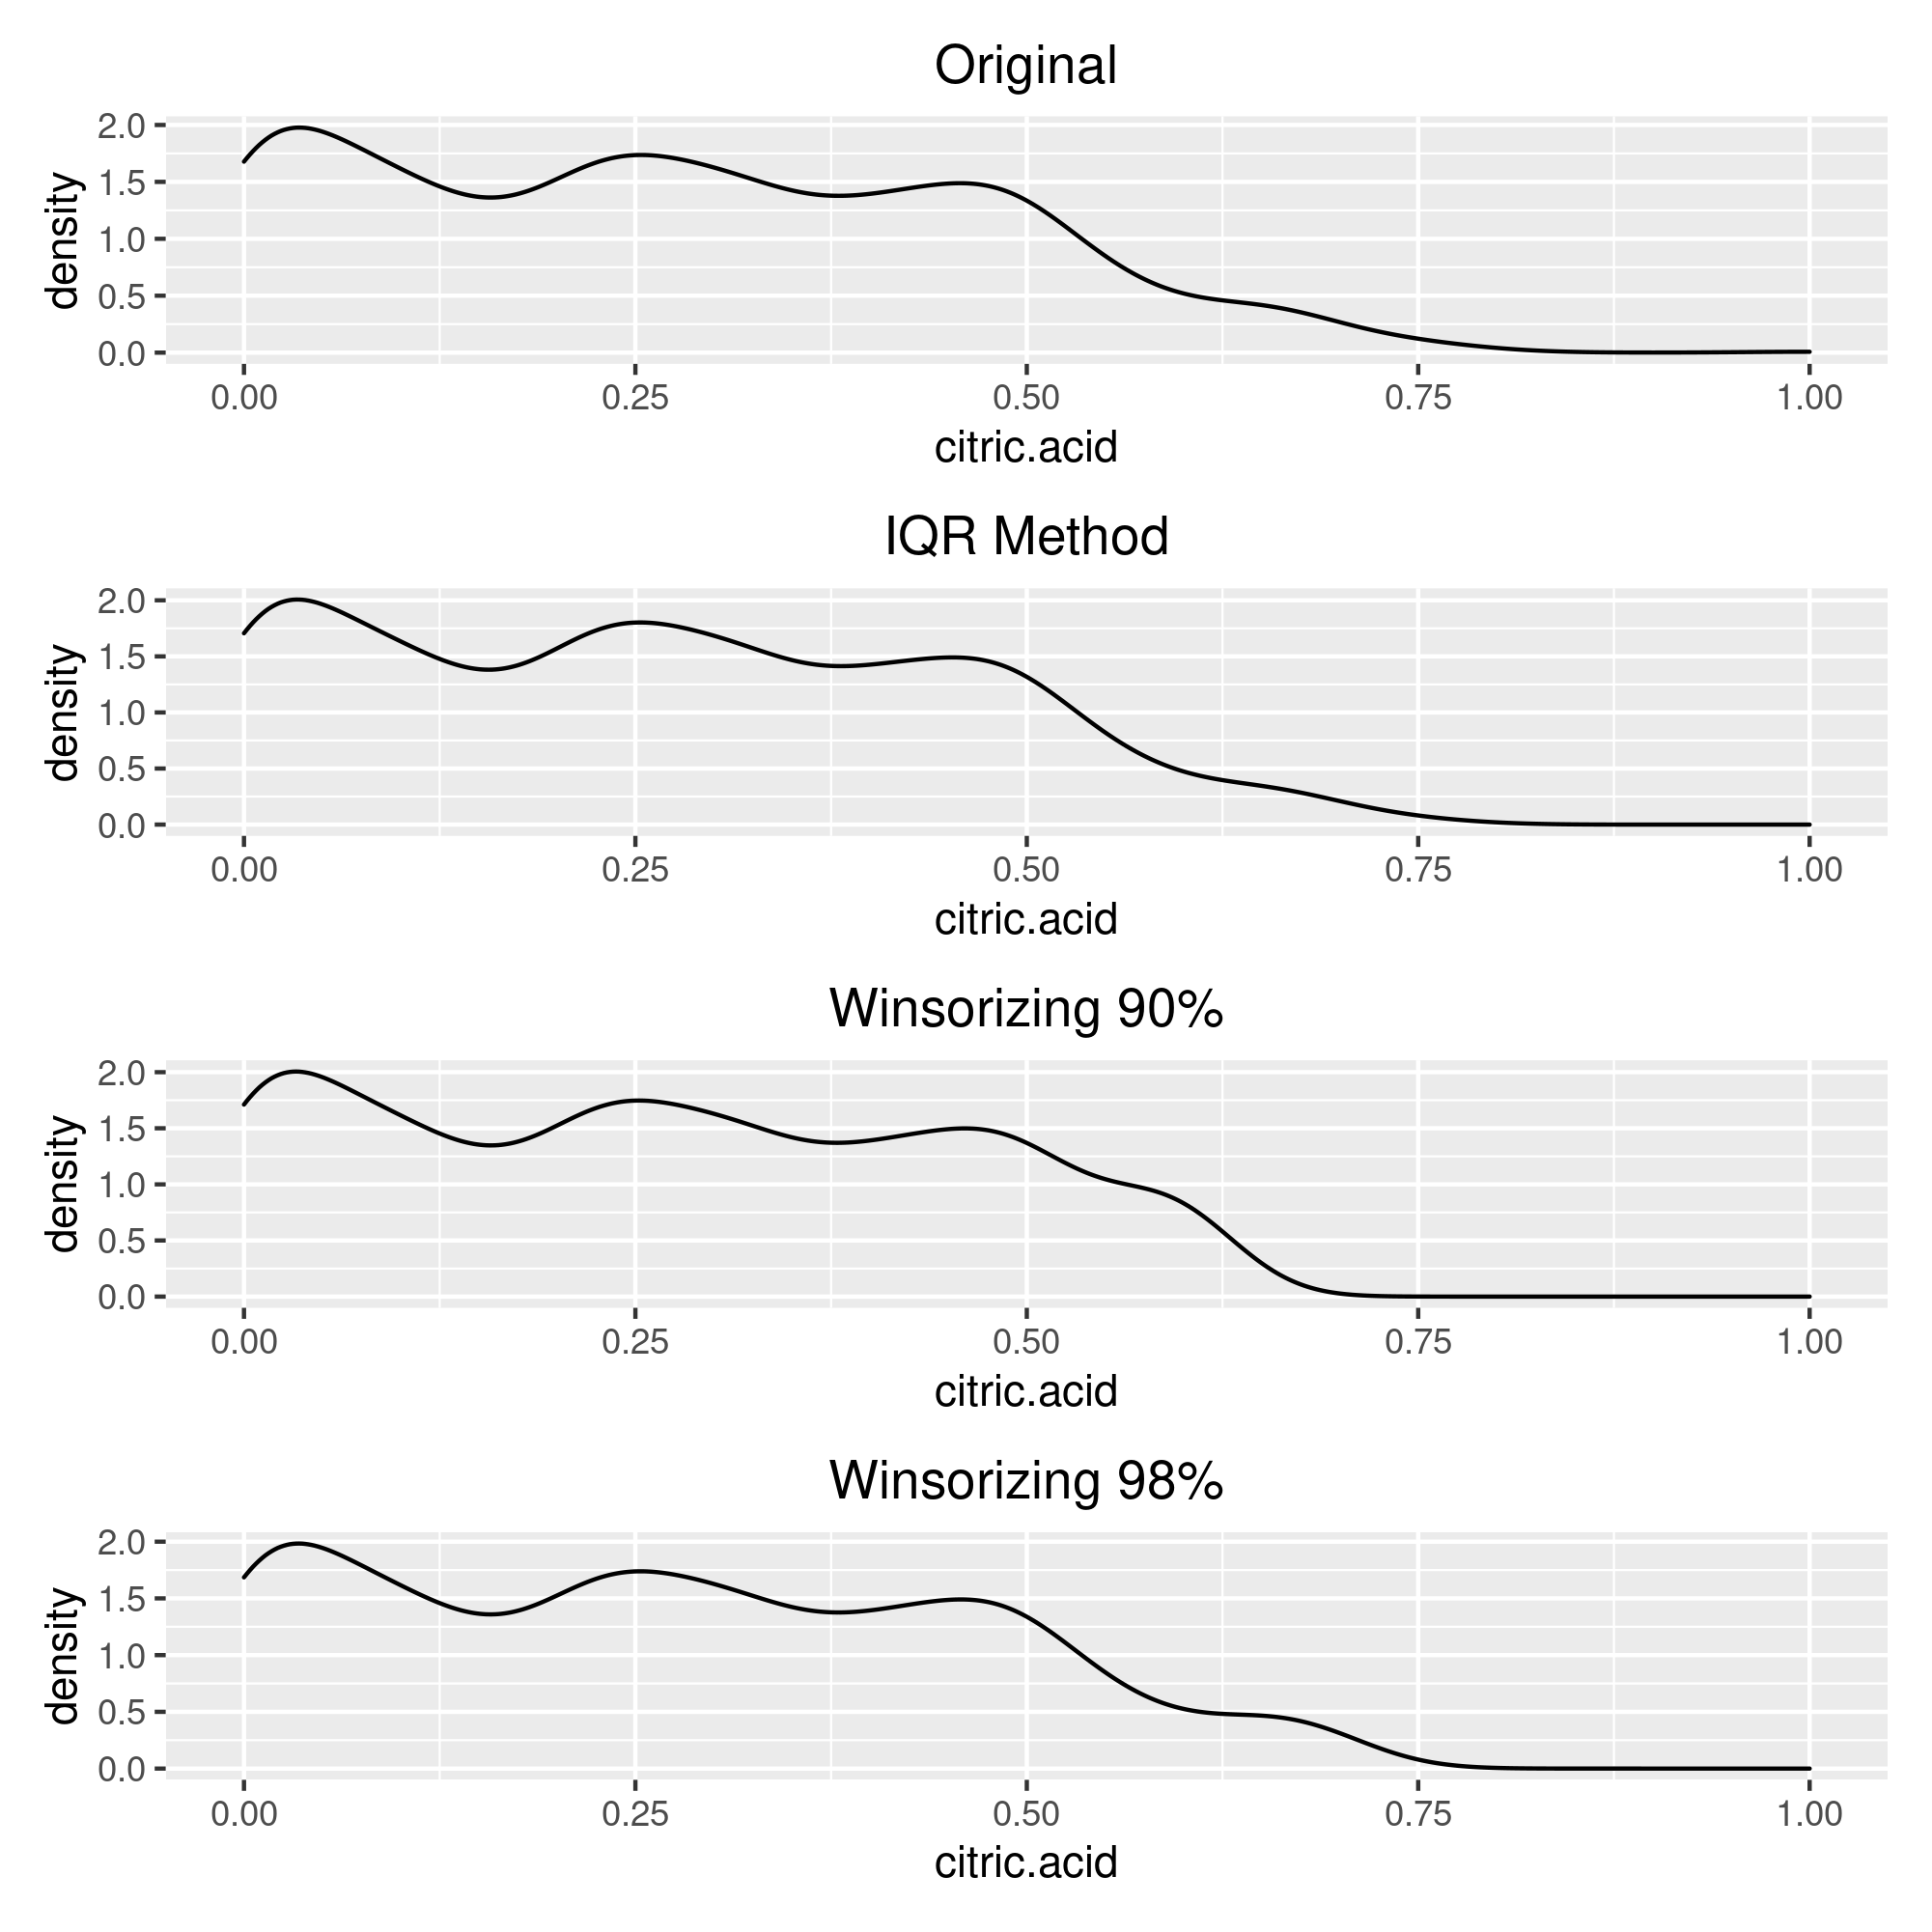
\includegraphics[width=0.45\textwidth]{images/outliers/citric.acid_distribution.png}
    }\qquad
    \subfloat[]{%
        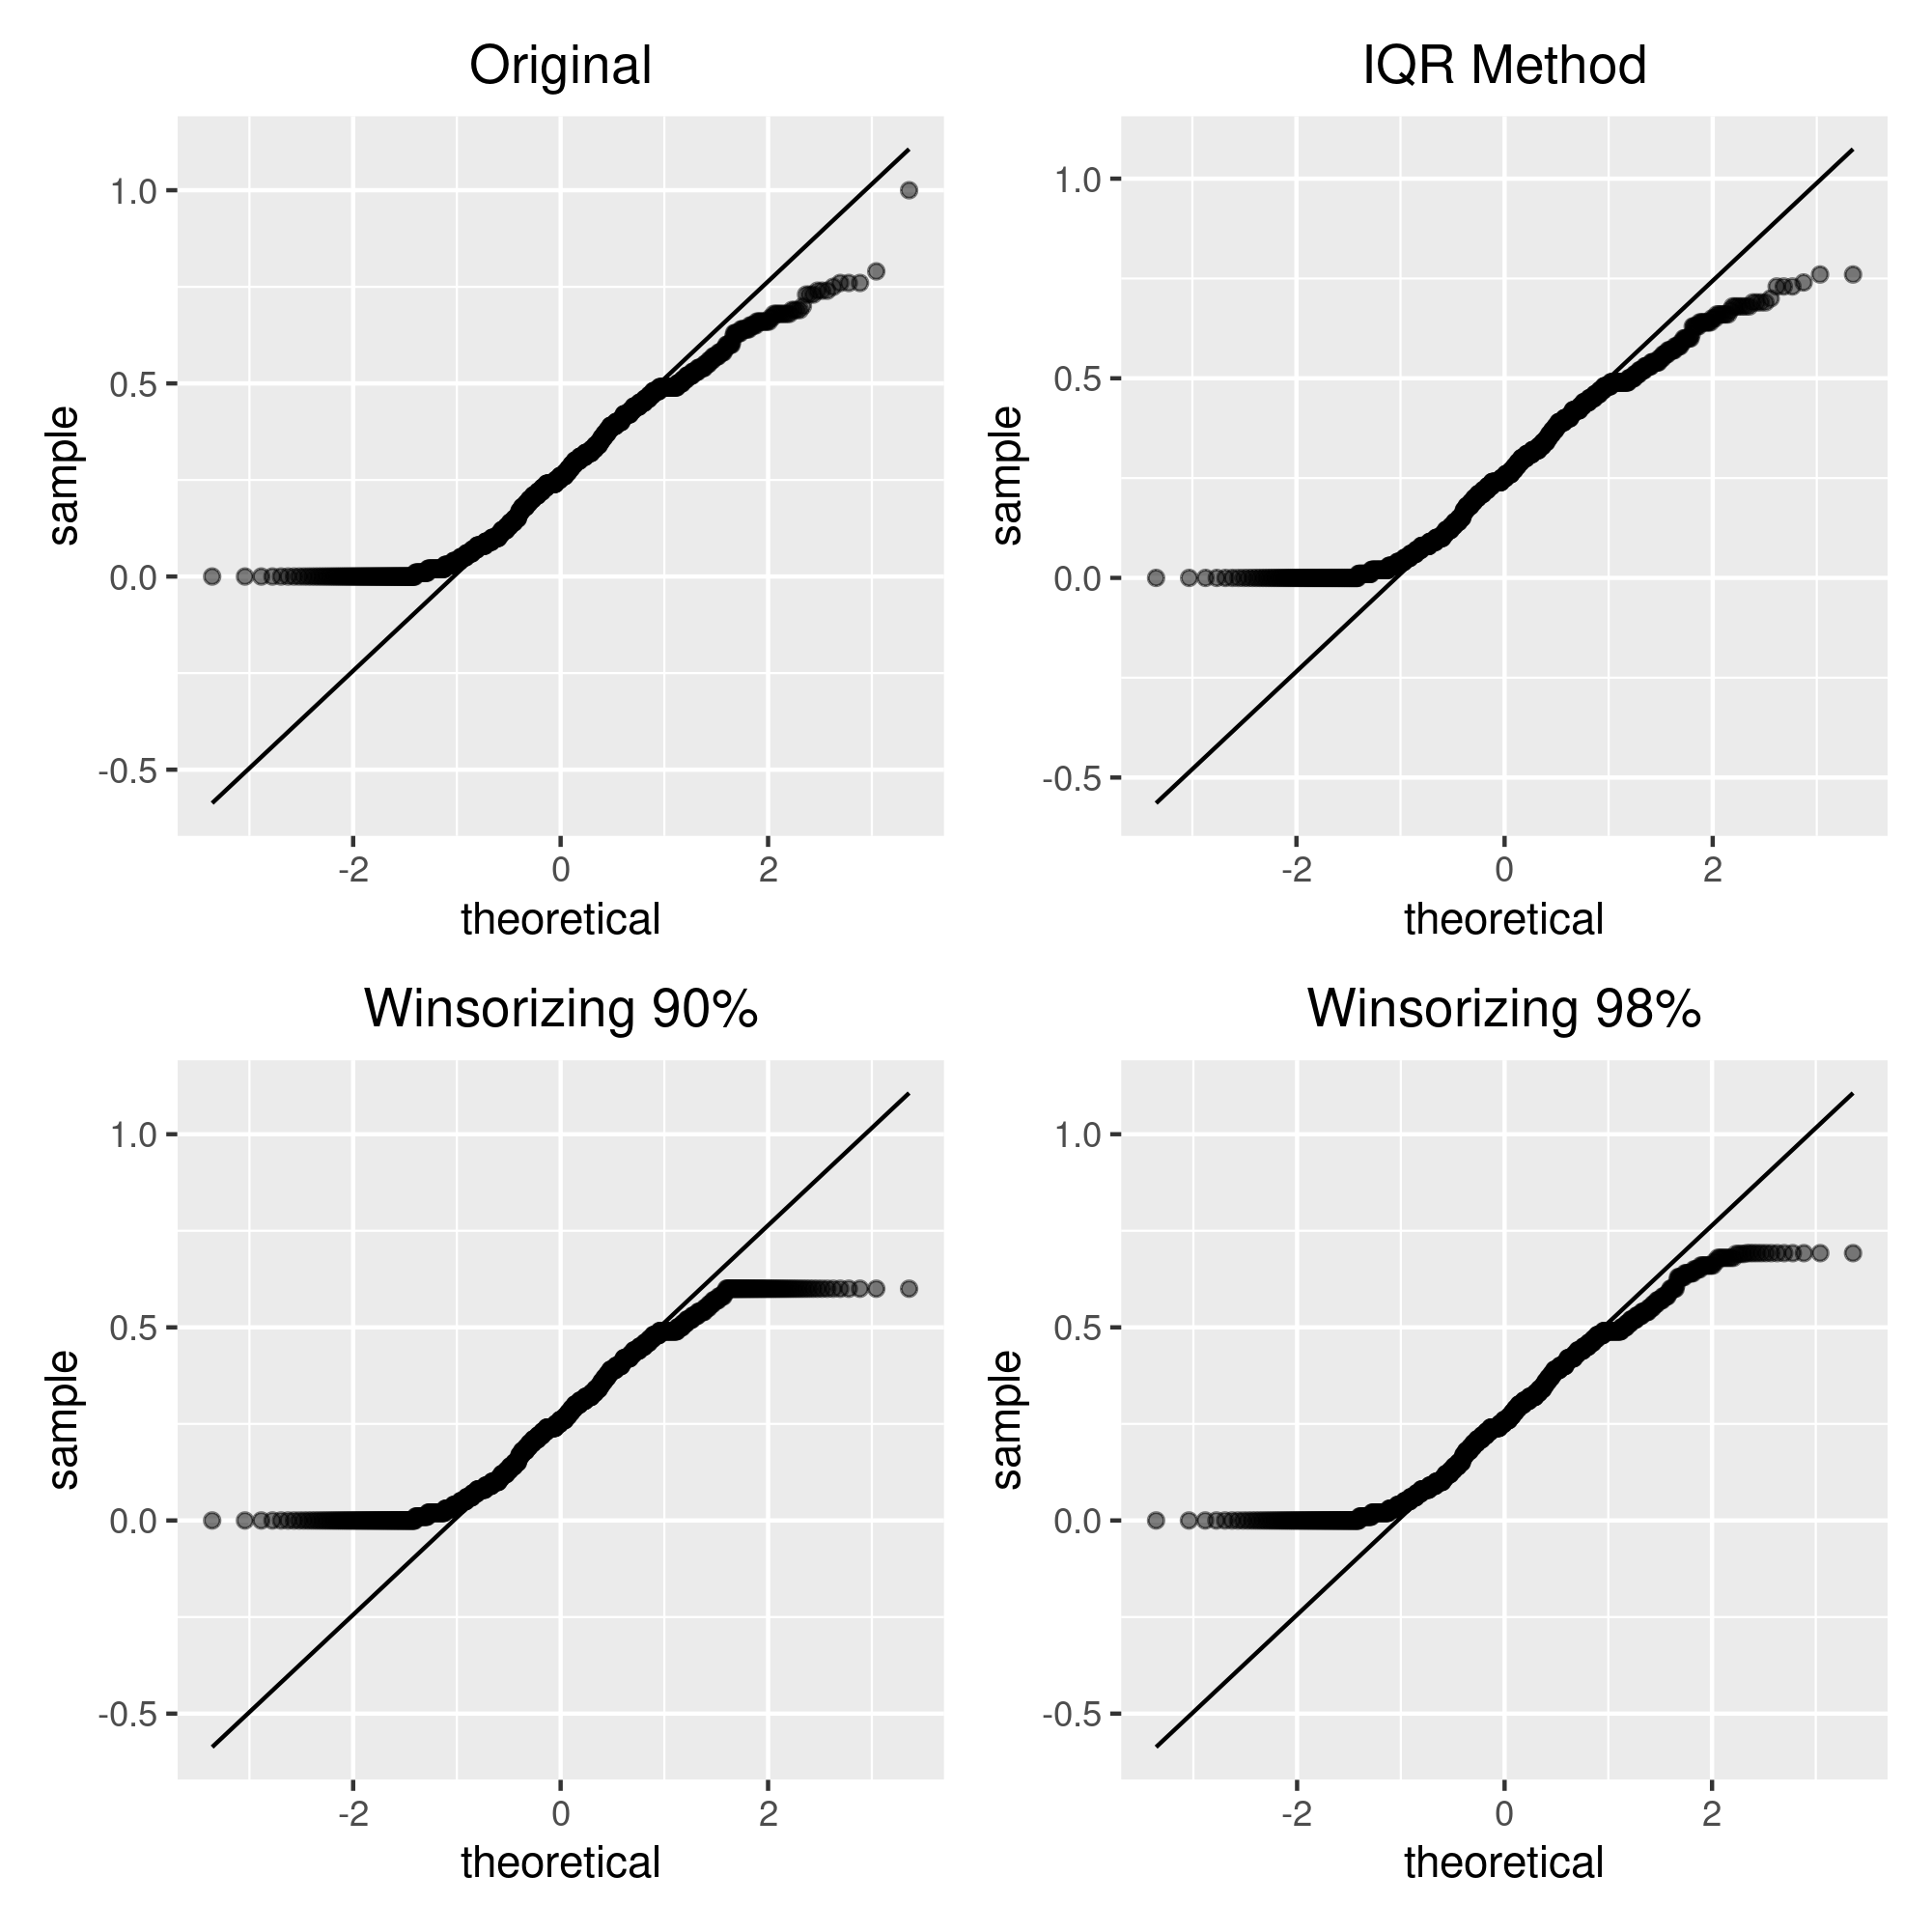
\includegraphics[width=0.45\textwidth]{images/outliers/citric.acid_qqplot.png}
    }

    \label{fig:citric.acid}
    \caption{Commento}
\end{figure}

\begin{figure}[H]
    \centering

    \subfloat[]{%
        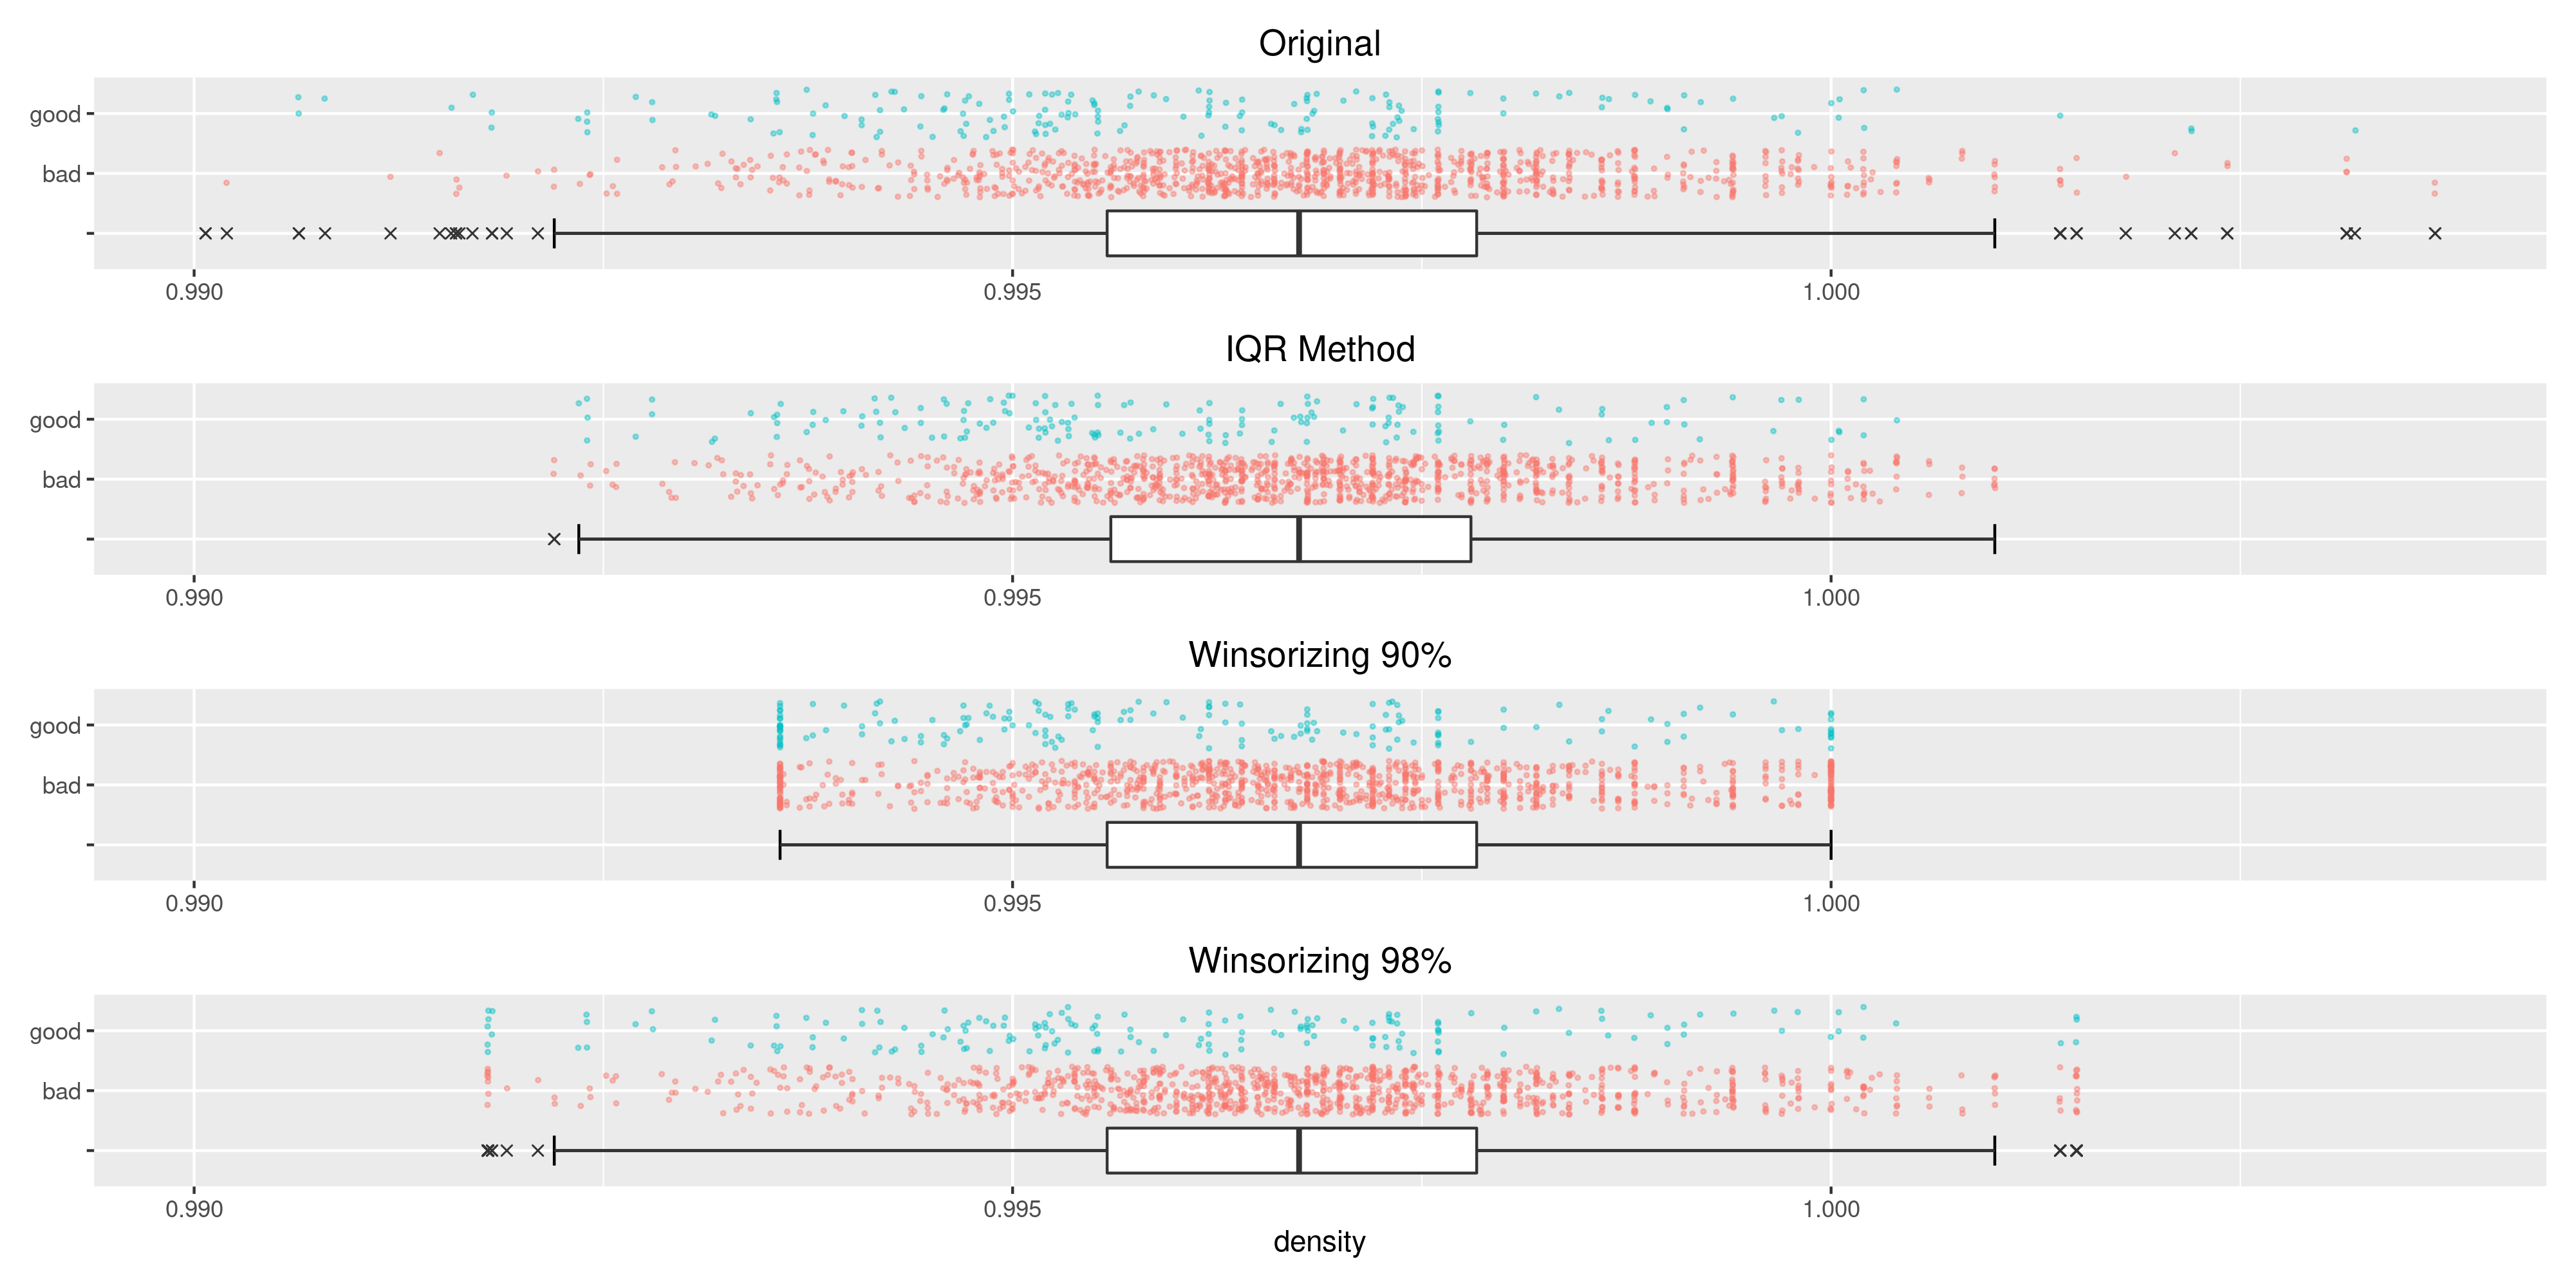
\includegraphics[width=0.99\textwidth]{images/outliers/density_boxplot.png}
    }

    \subfloat[]{%
        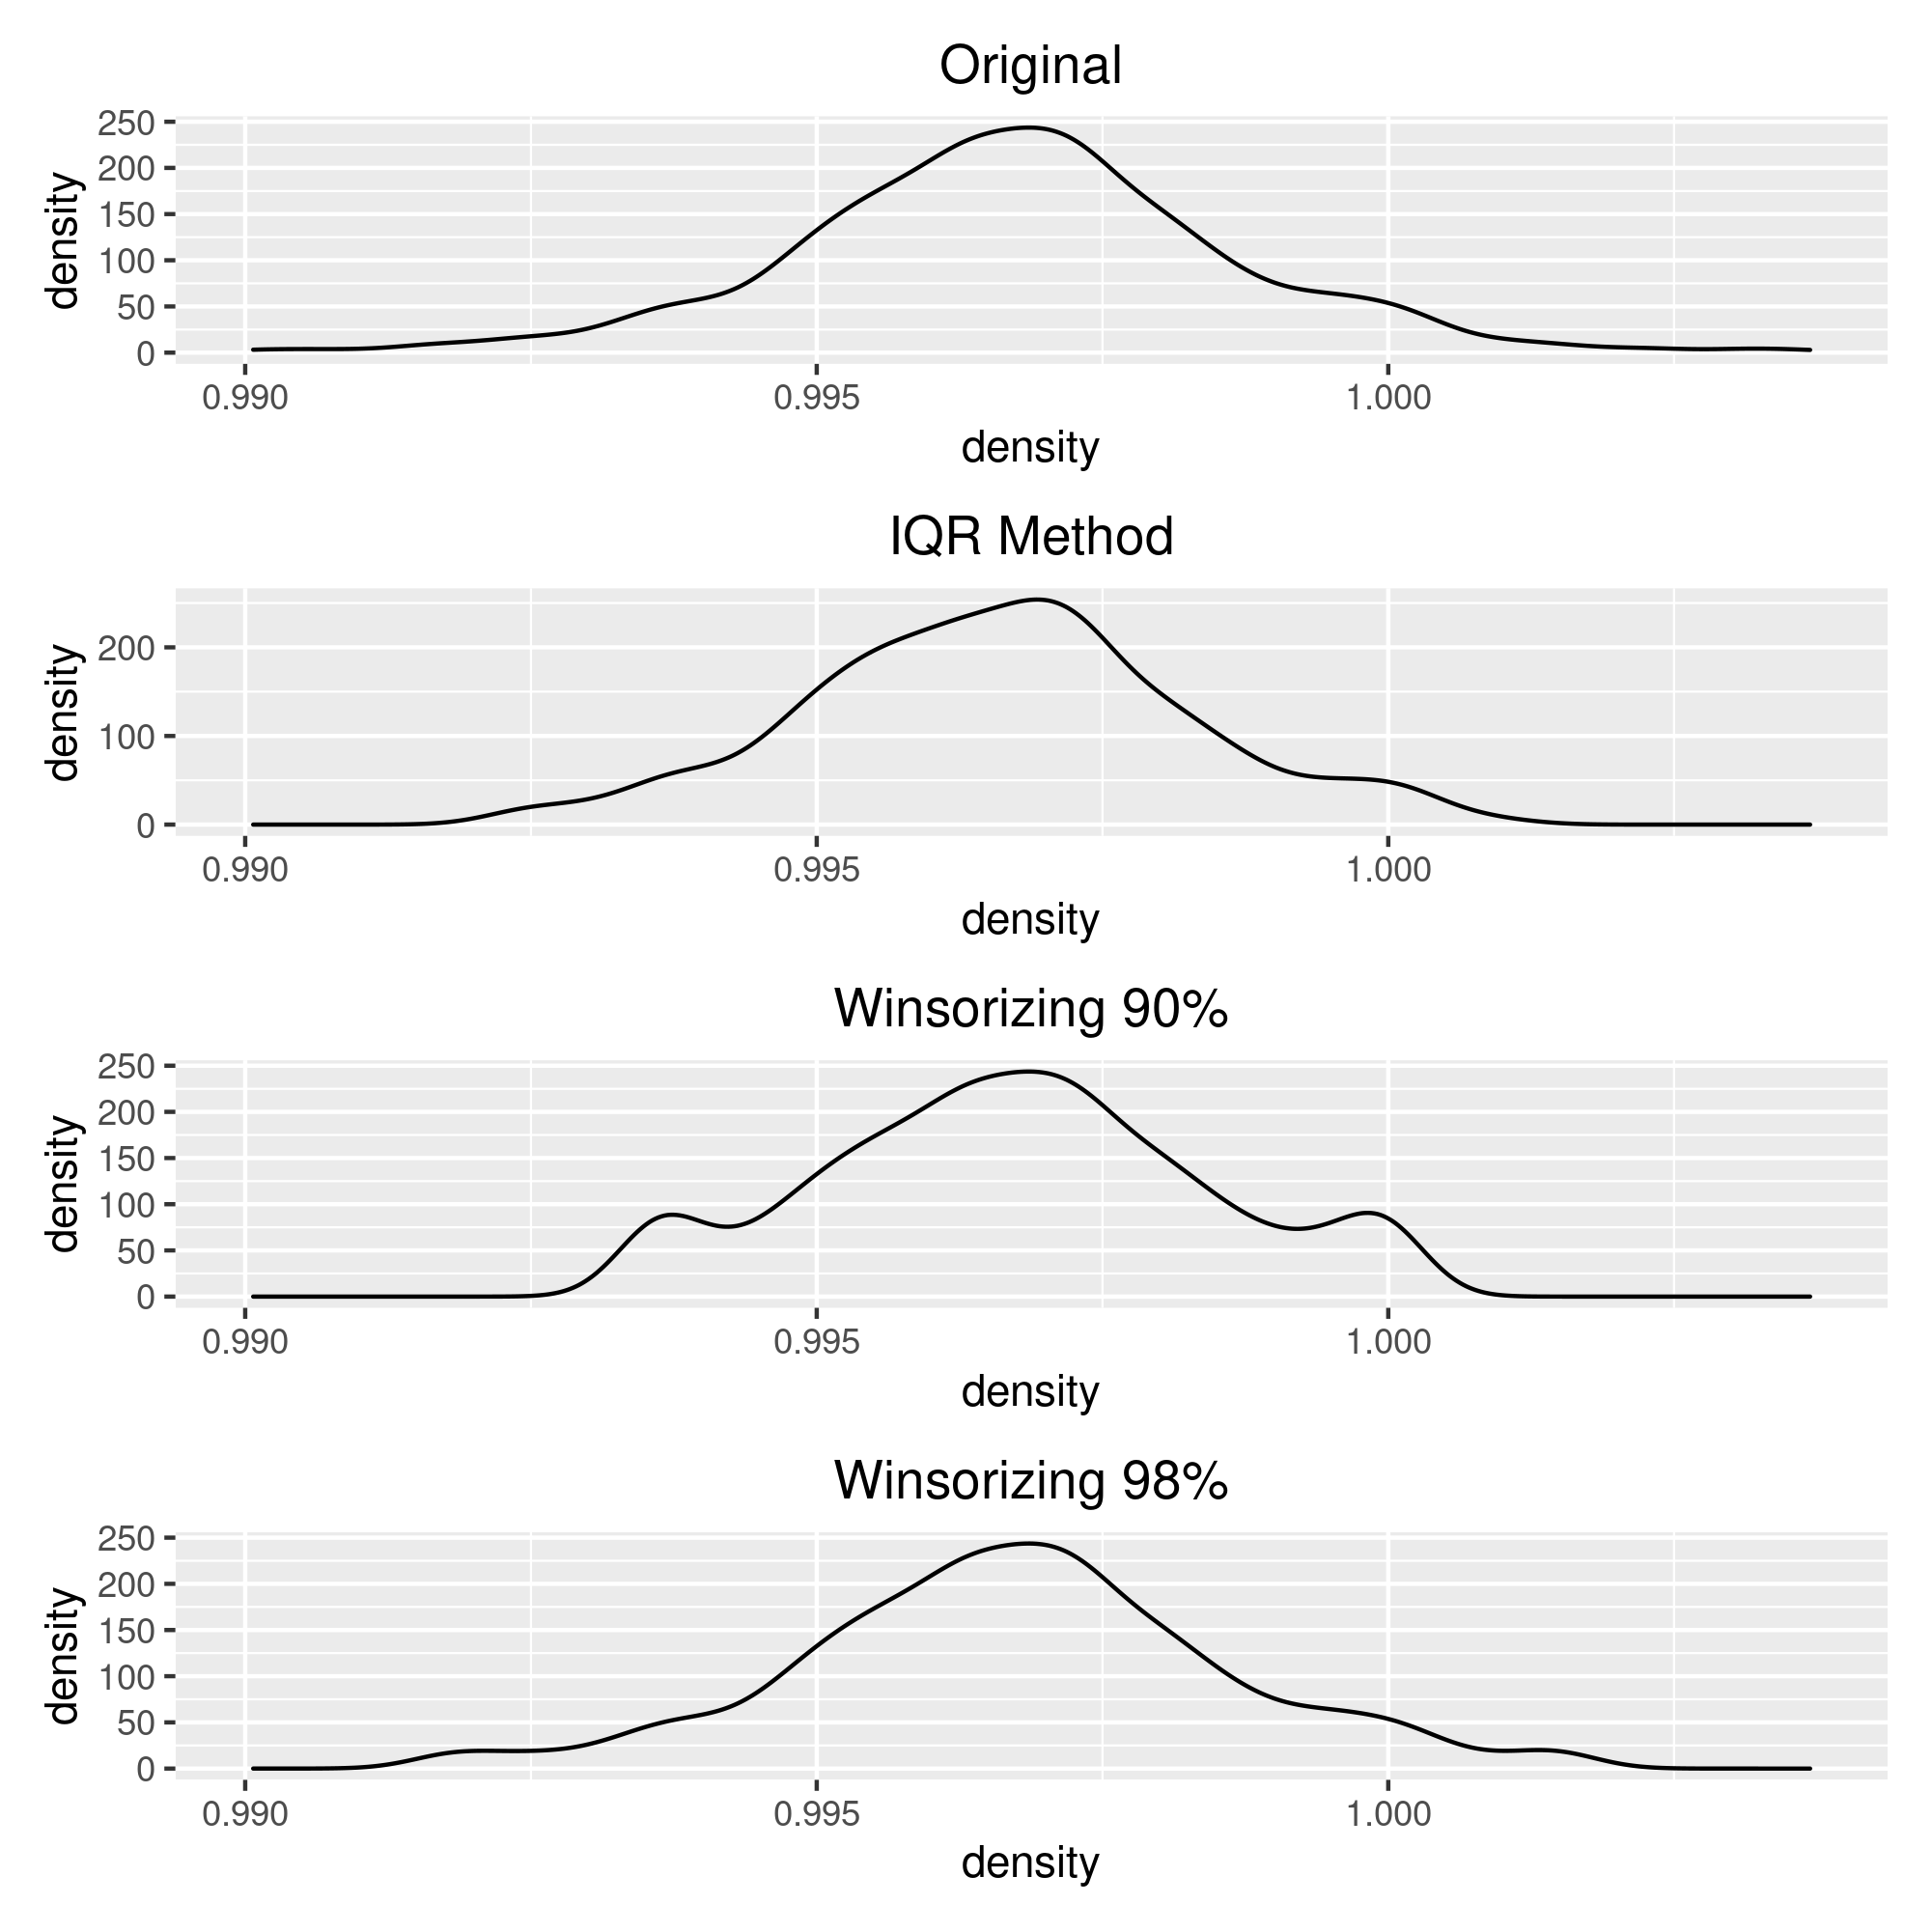
\includegraphics[width=0.45\textwidth]{images/outliers/density_distribution.png}
    }\qquad
    \subfloat[]{%
        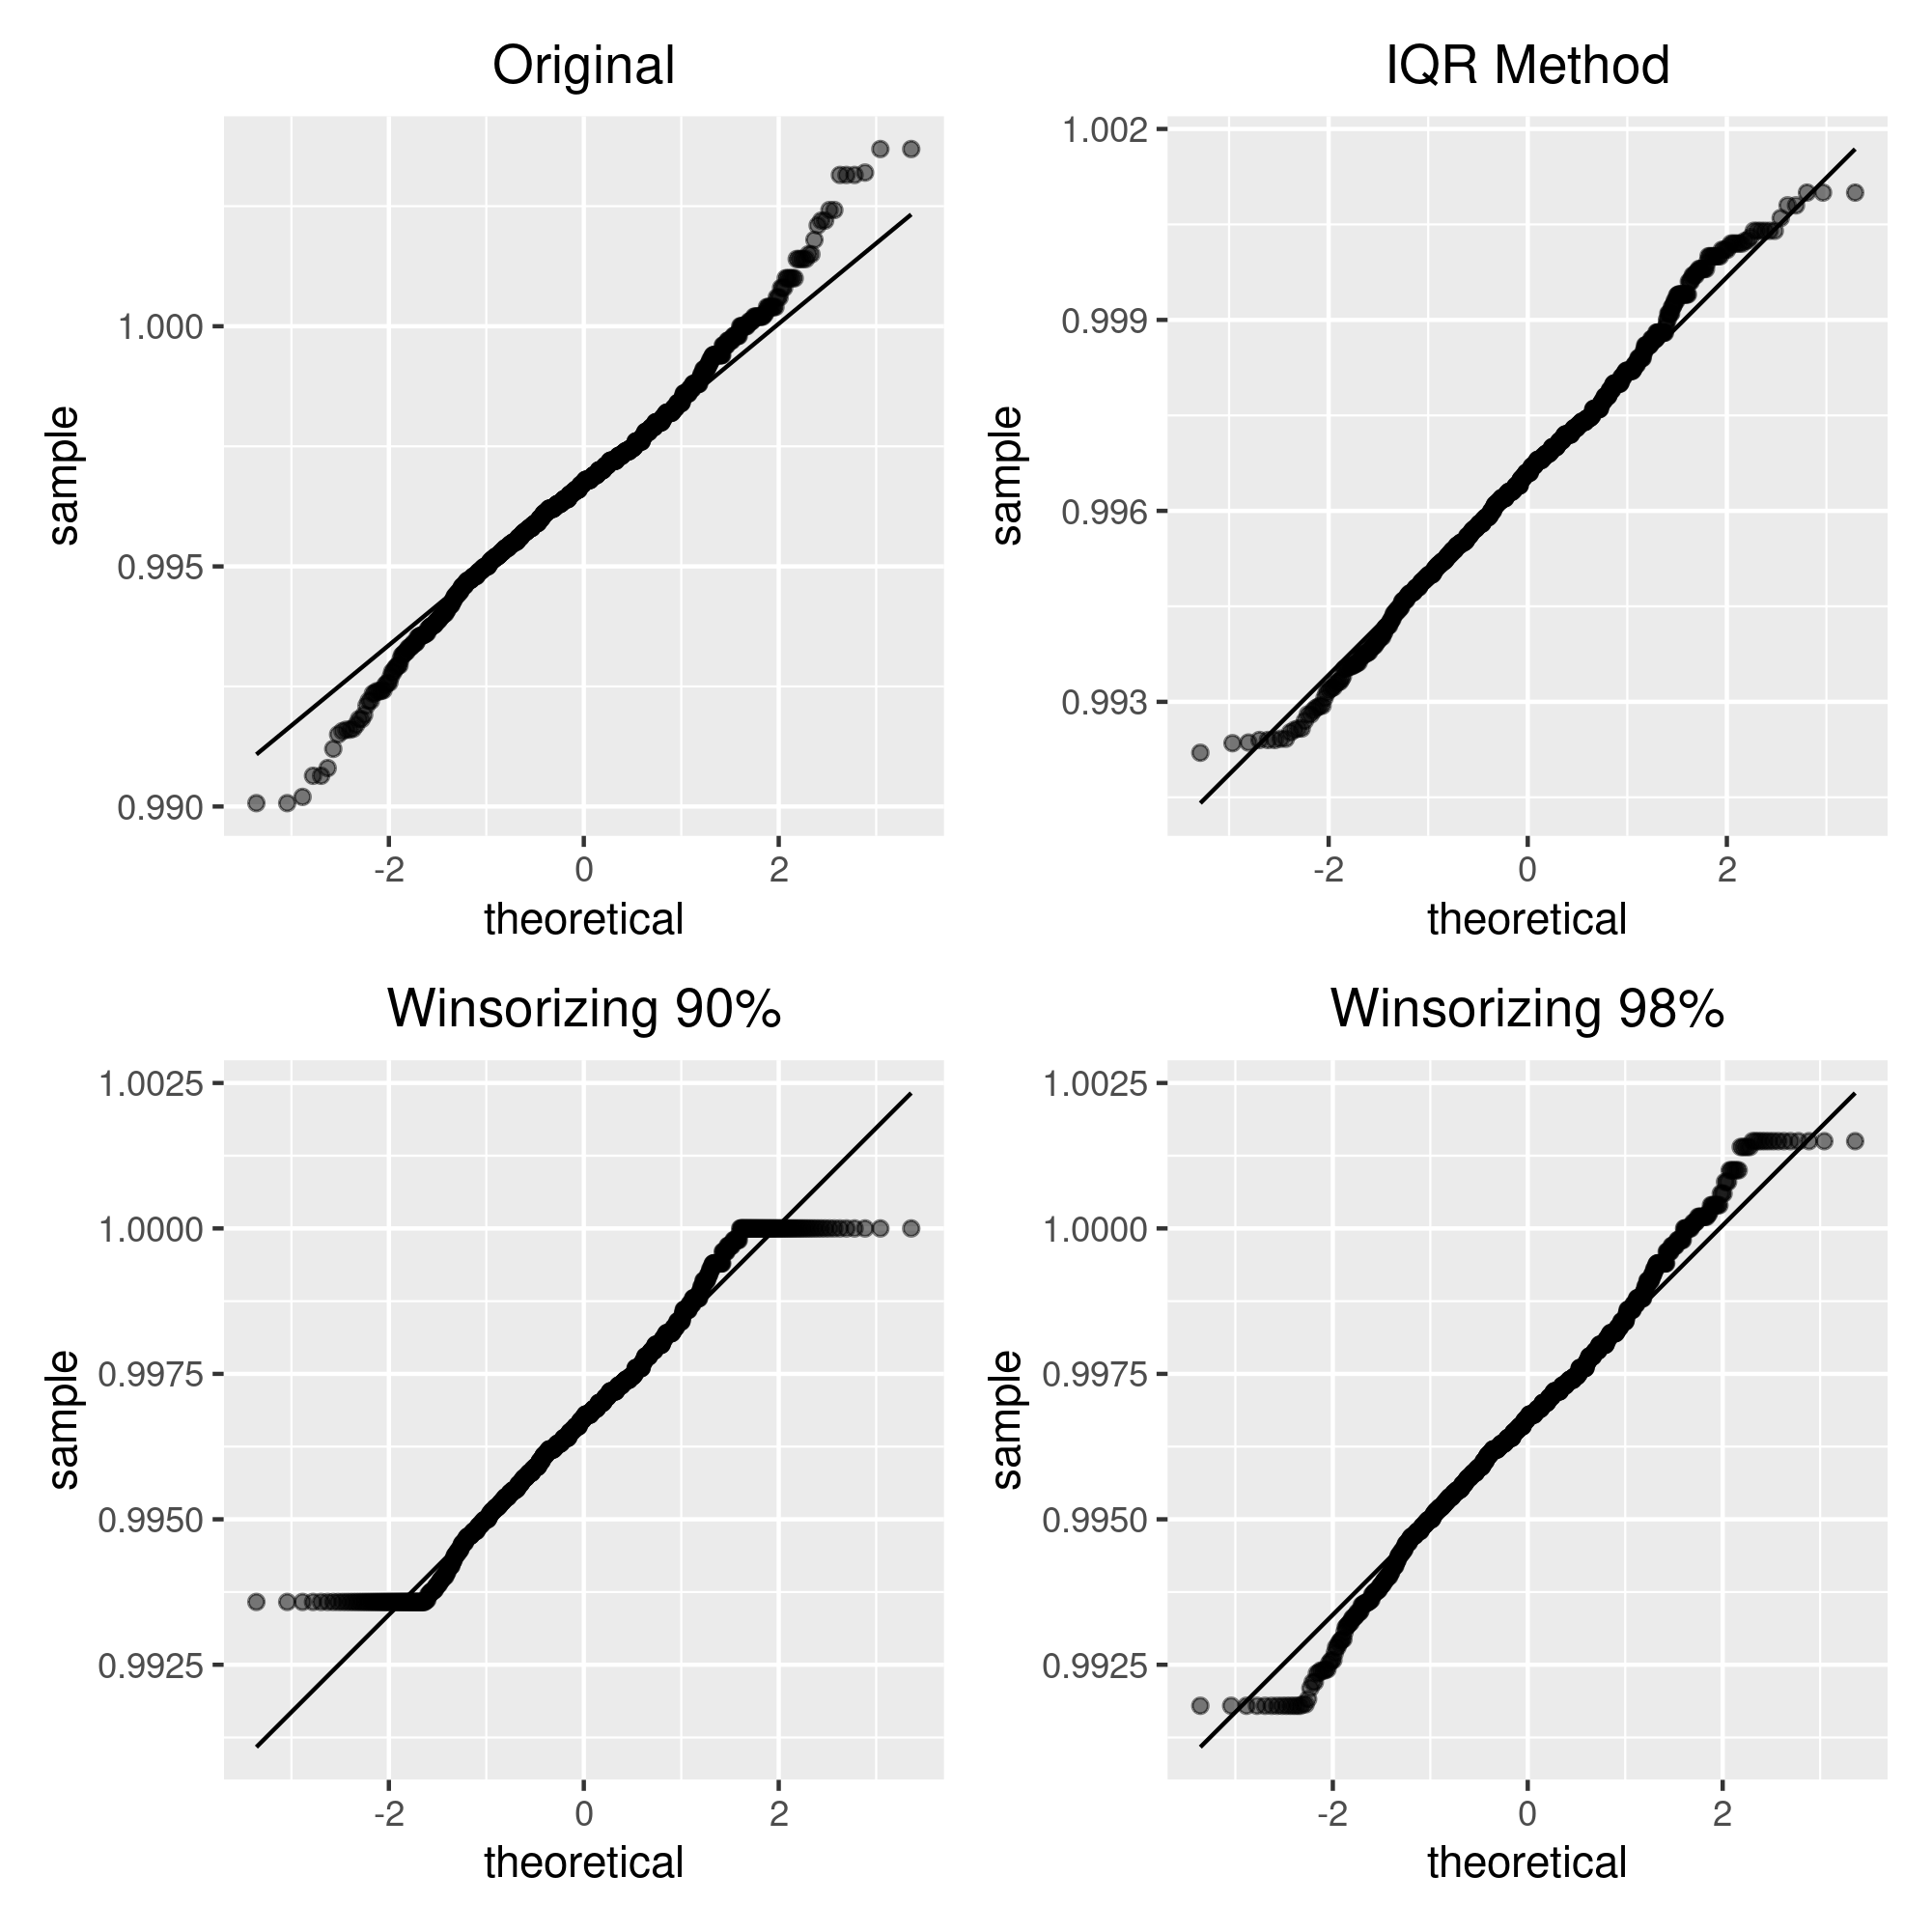
\includegraphics[width=0.45\textwidth]{images/outliers/density_qqplot.png}
    }

    \label{fig:density}
    \caption{Commento}
\end{figure}

\begin{figure}[H]
    \centering

    \subfloat[]{%
        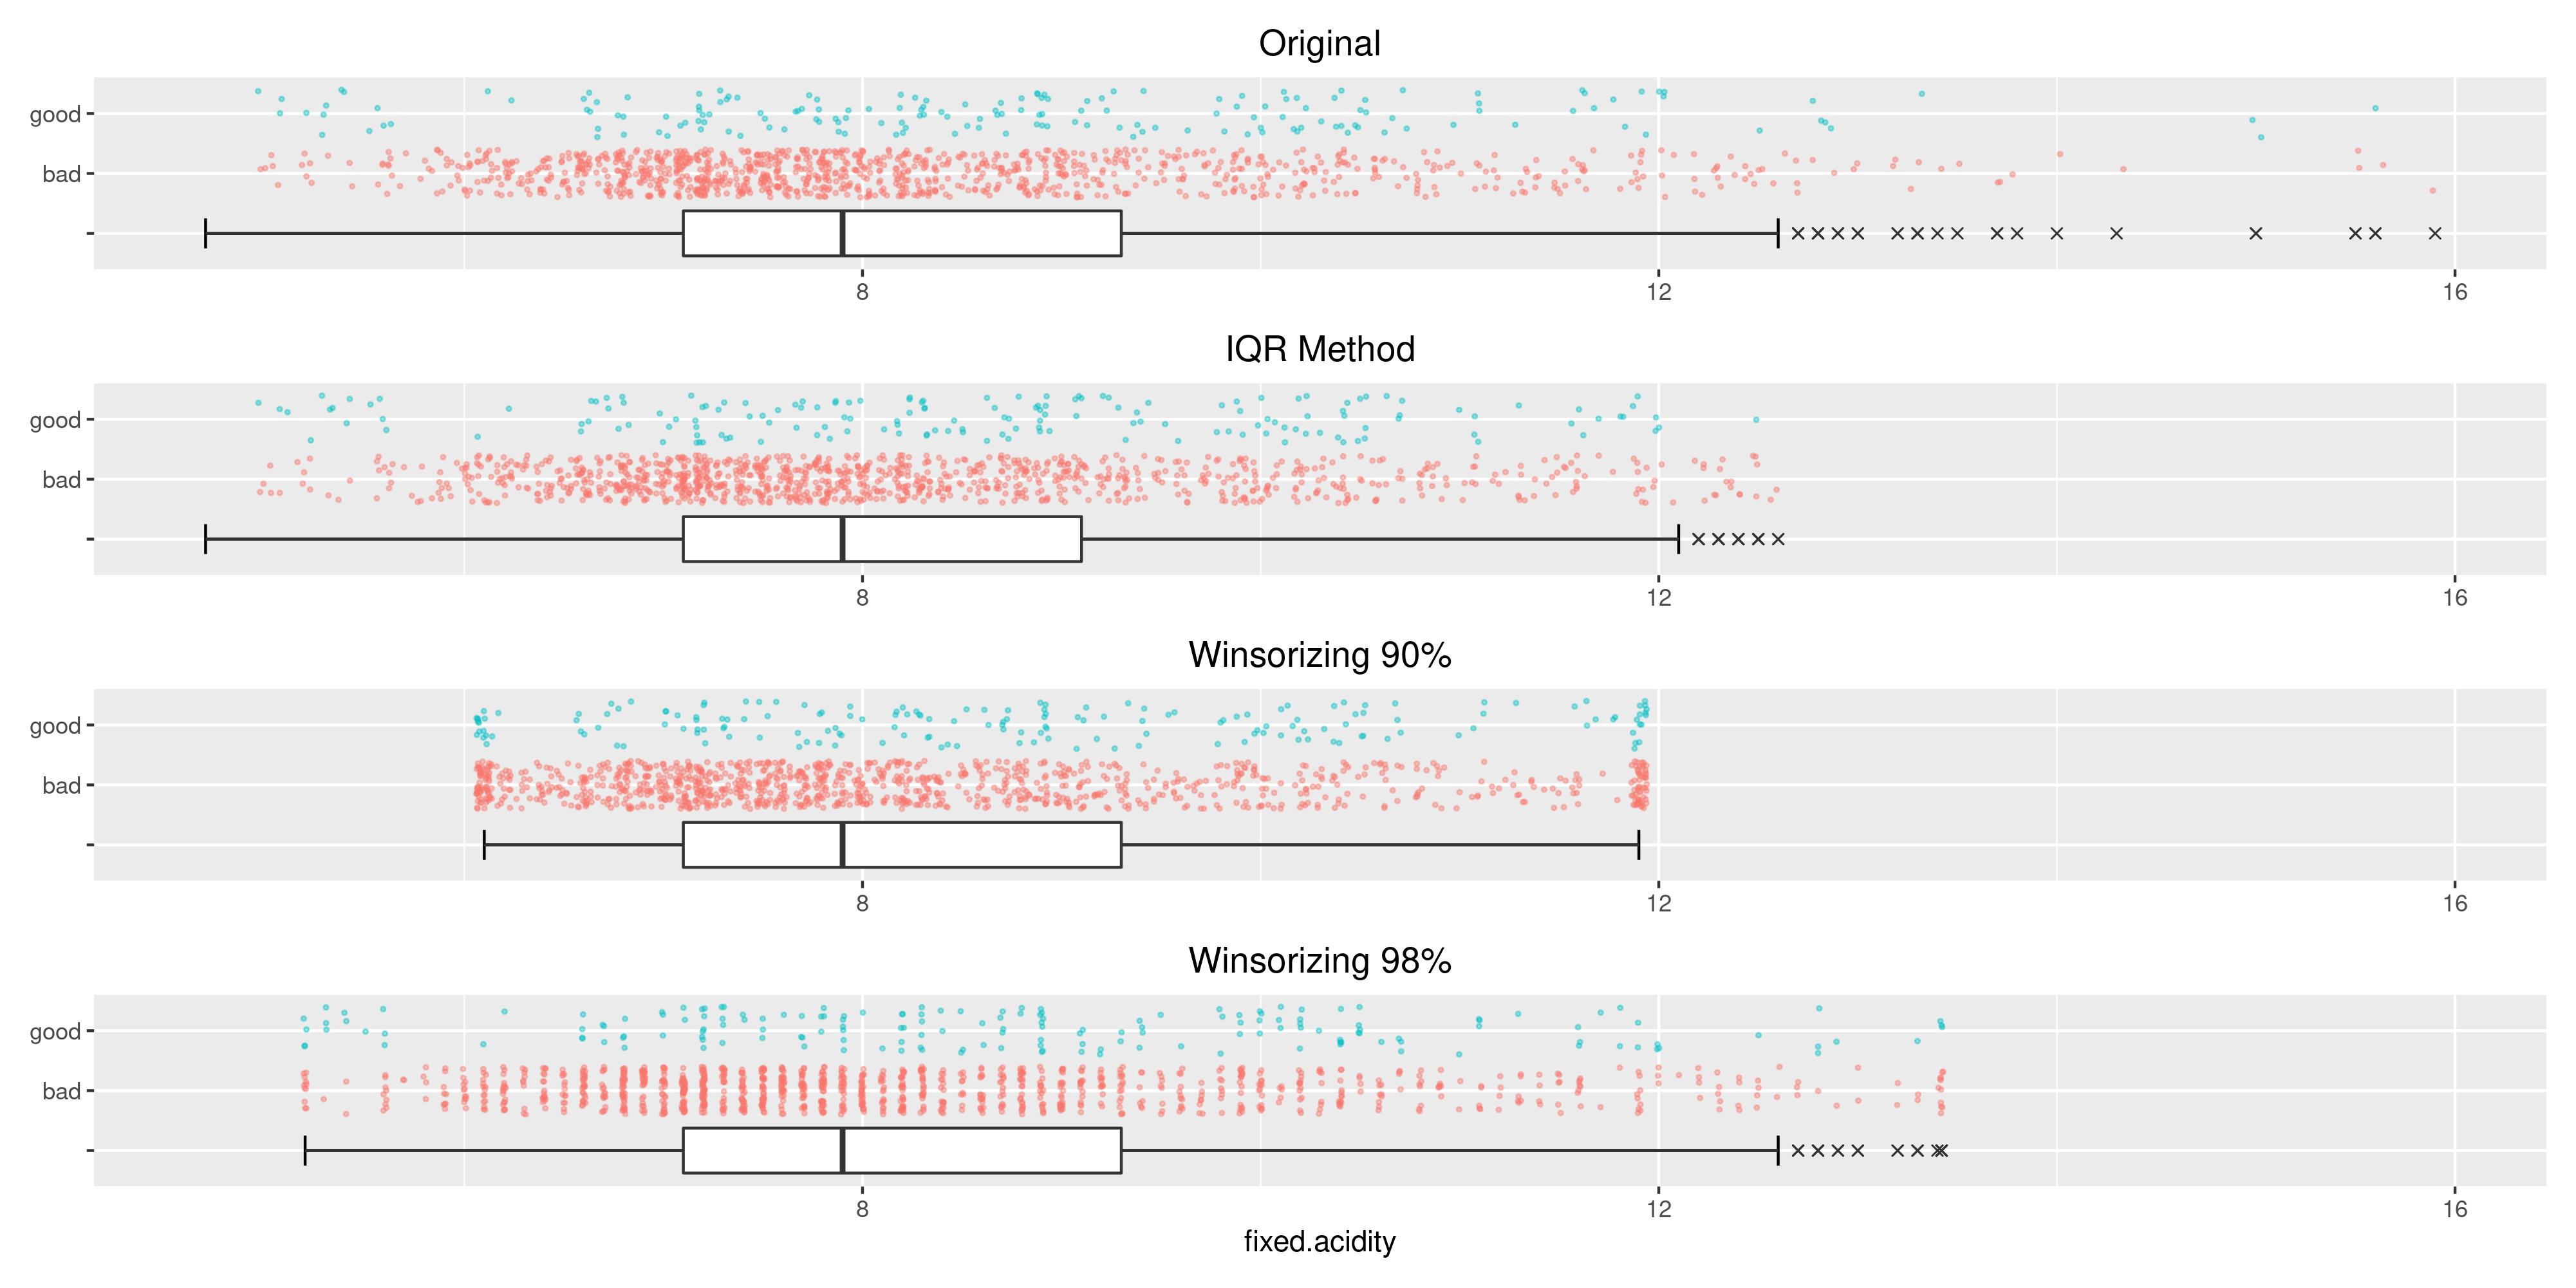
\includegraphics[width=0.99\textwidth]{images/outliers/fixed.acidity_boxplot.png}
    }

    \subfloat[]{%
        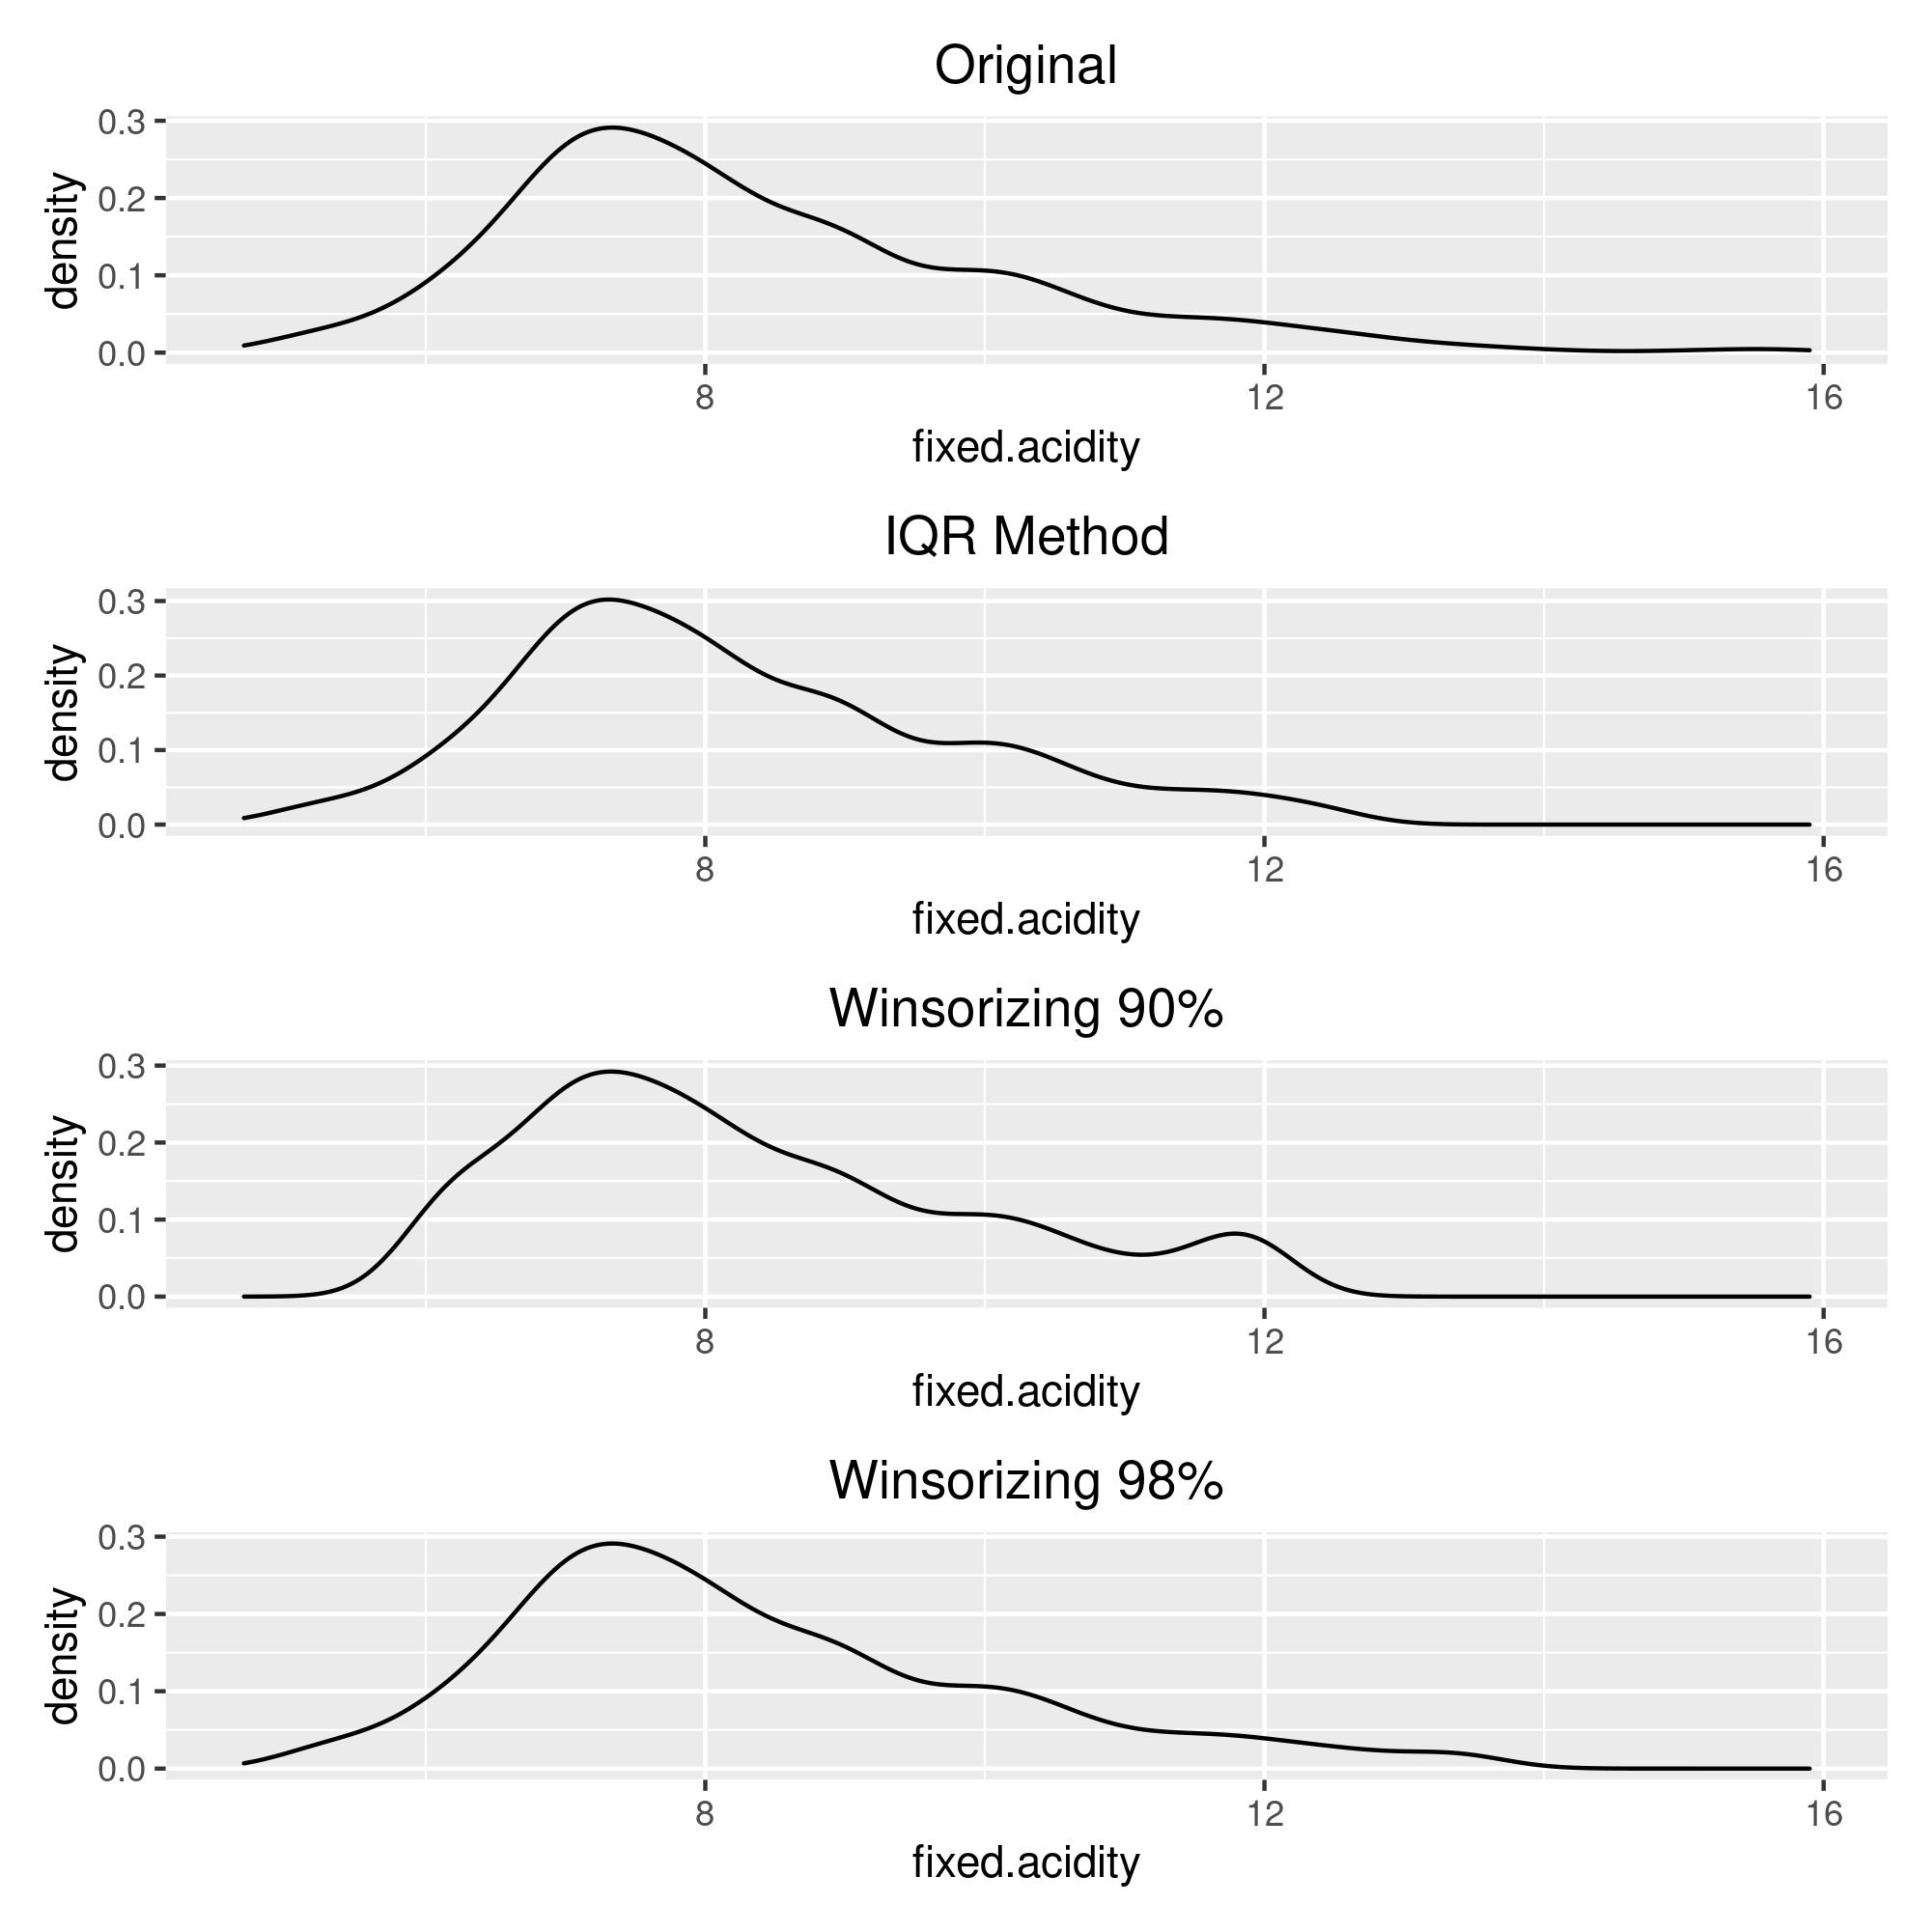
\includegraphics[width=0.45\textwidth]{images/outliers/fixed.acidity_distribution.png}
    }\qquad
    \subfloat[]{%
        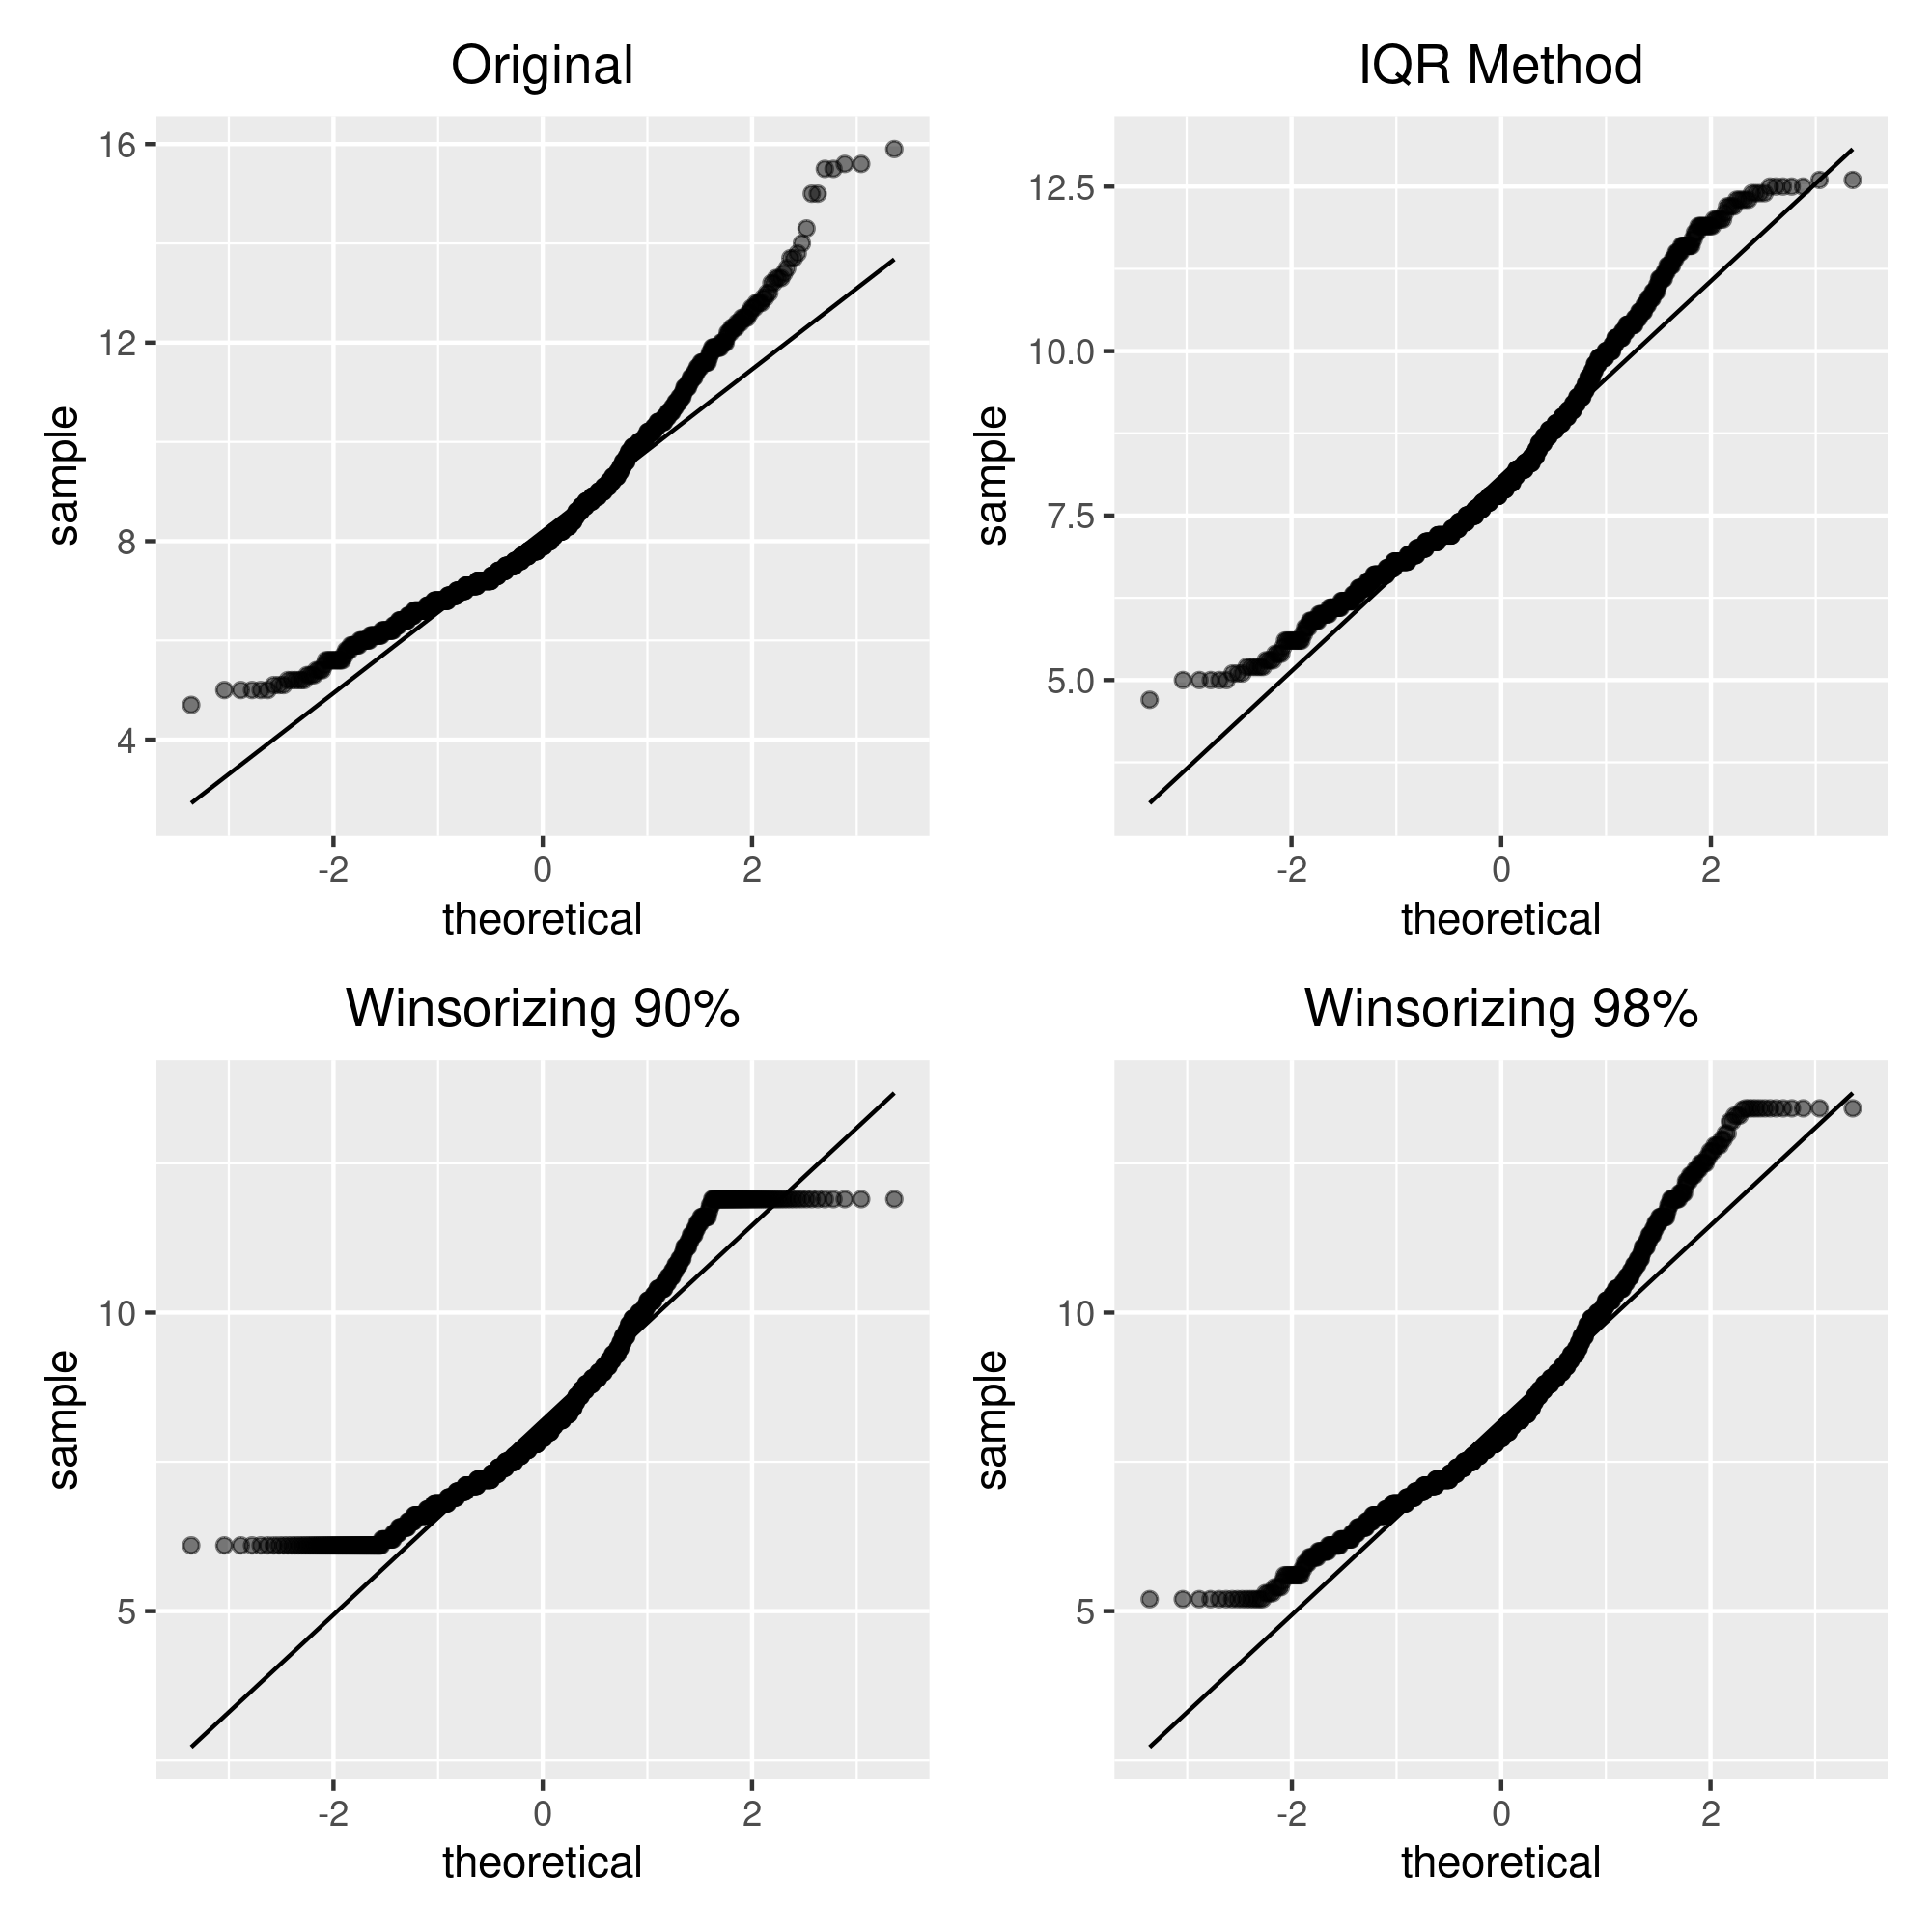
\includegraphics[width=0.45\textwidth]{images/outliers/fixed.acidity_qqplot.png}
    }

    \label{fig:fixed.acidity}
    \caption{Commento}
\end{figure}

\begin{figure}[H]
    \centering

    \subfloat[]{%
        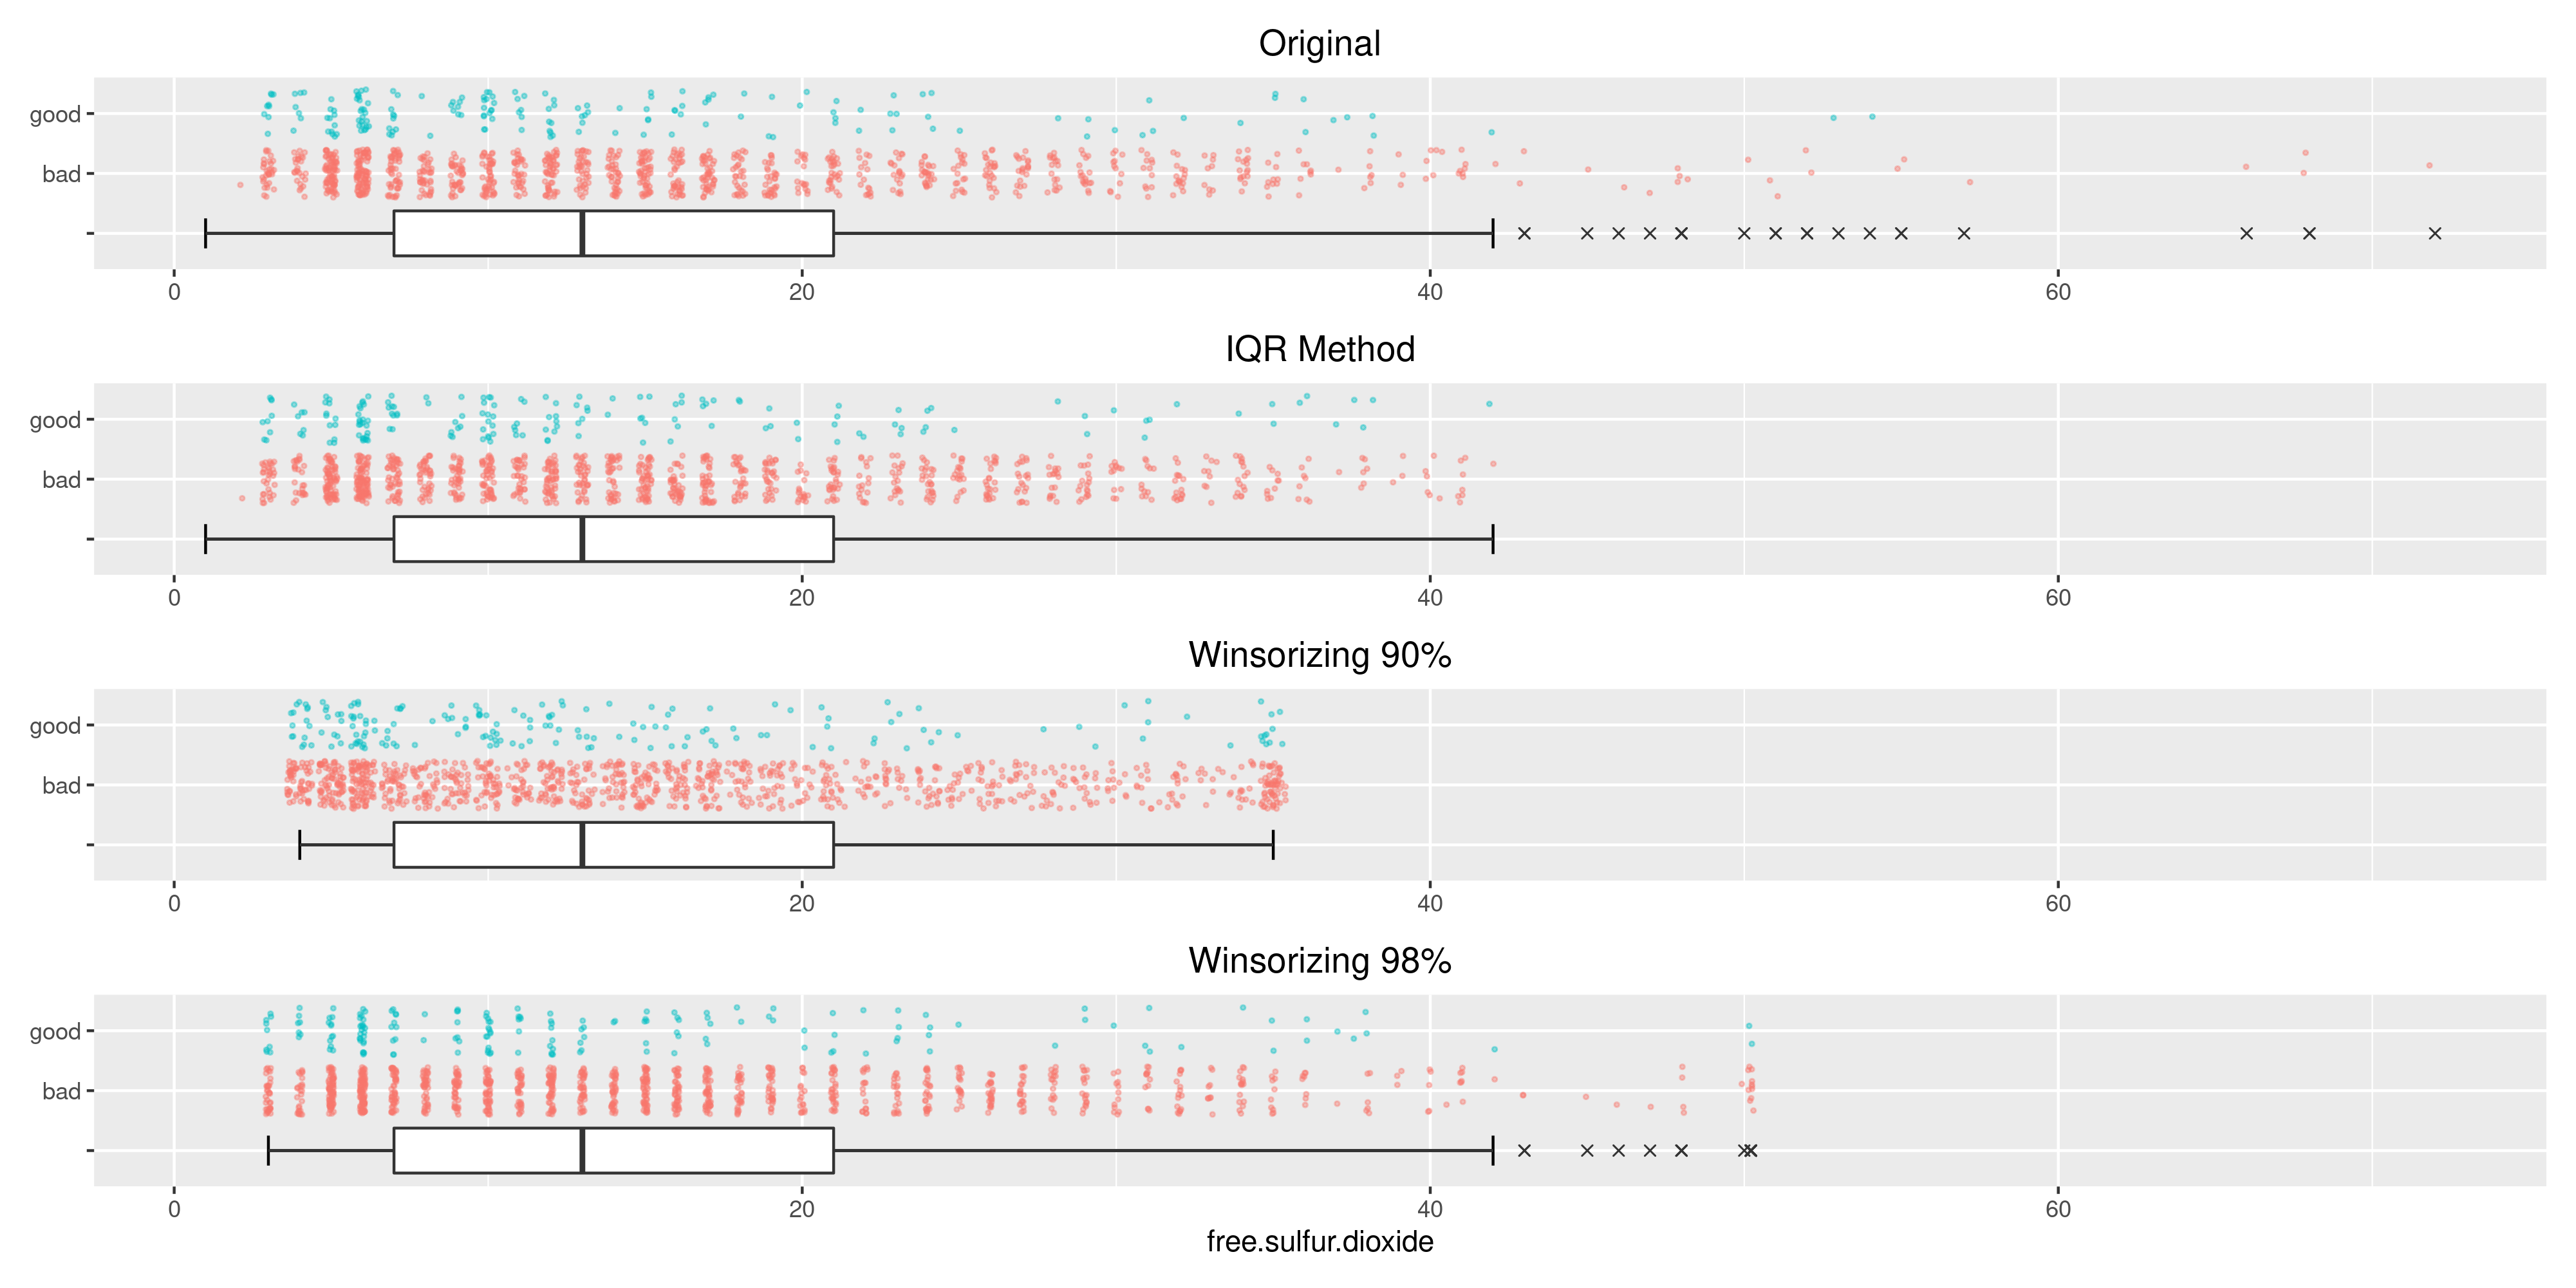
\includegraphics[width=0.99\textwidth]{images/outliers/free.sulfur.dioxide_boxplot.png}
    }

    \subfloat[]{%
        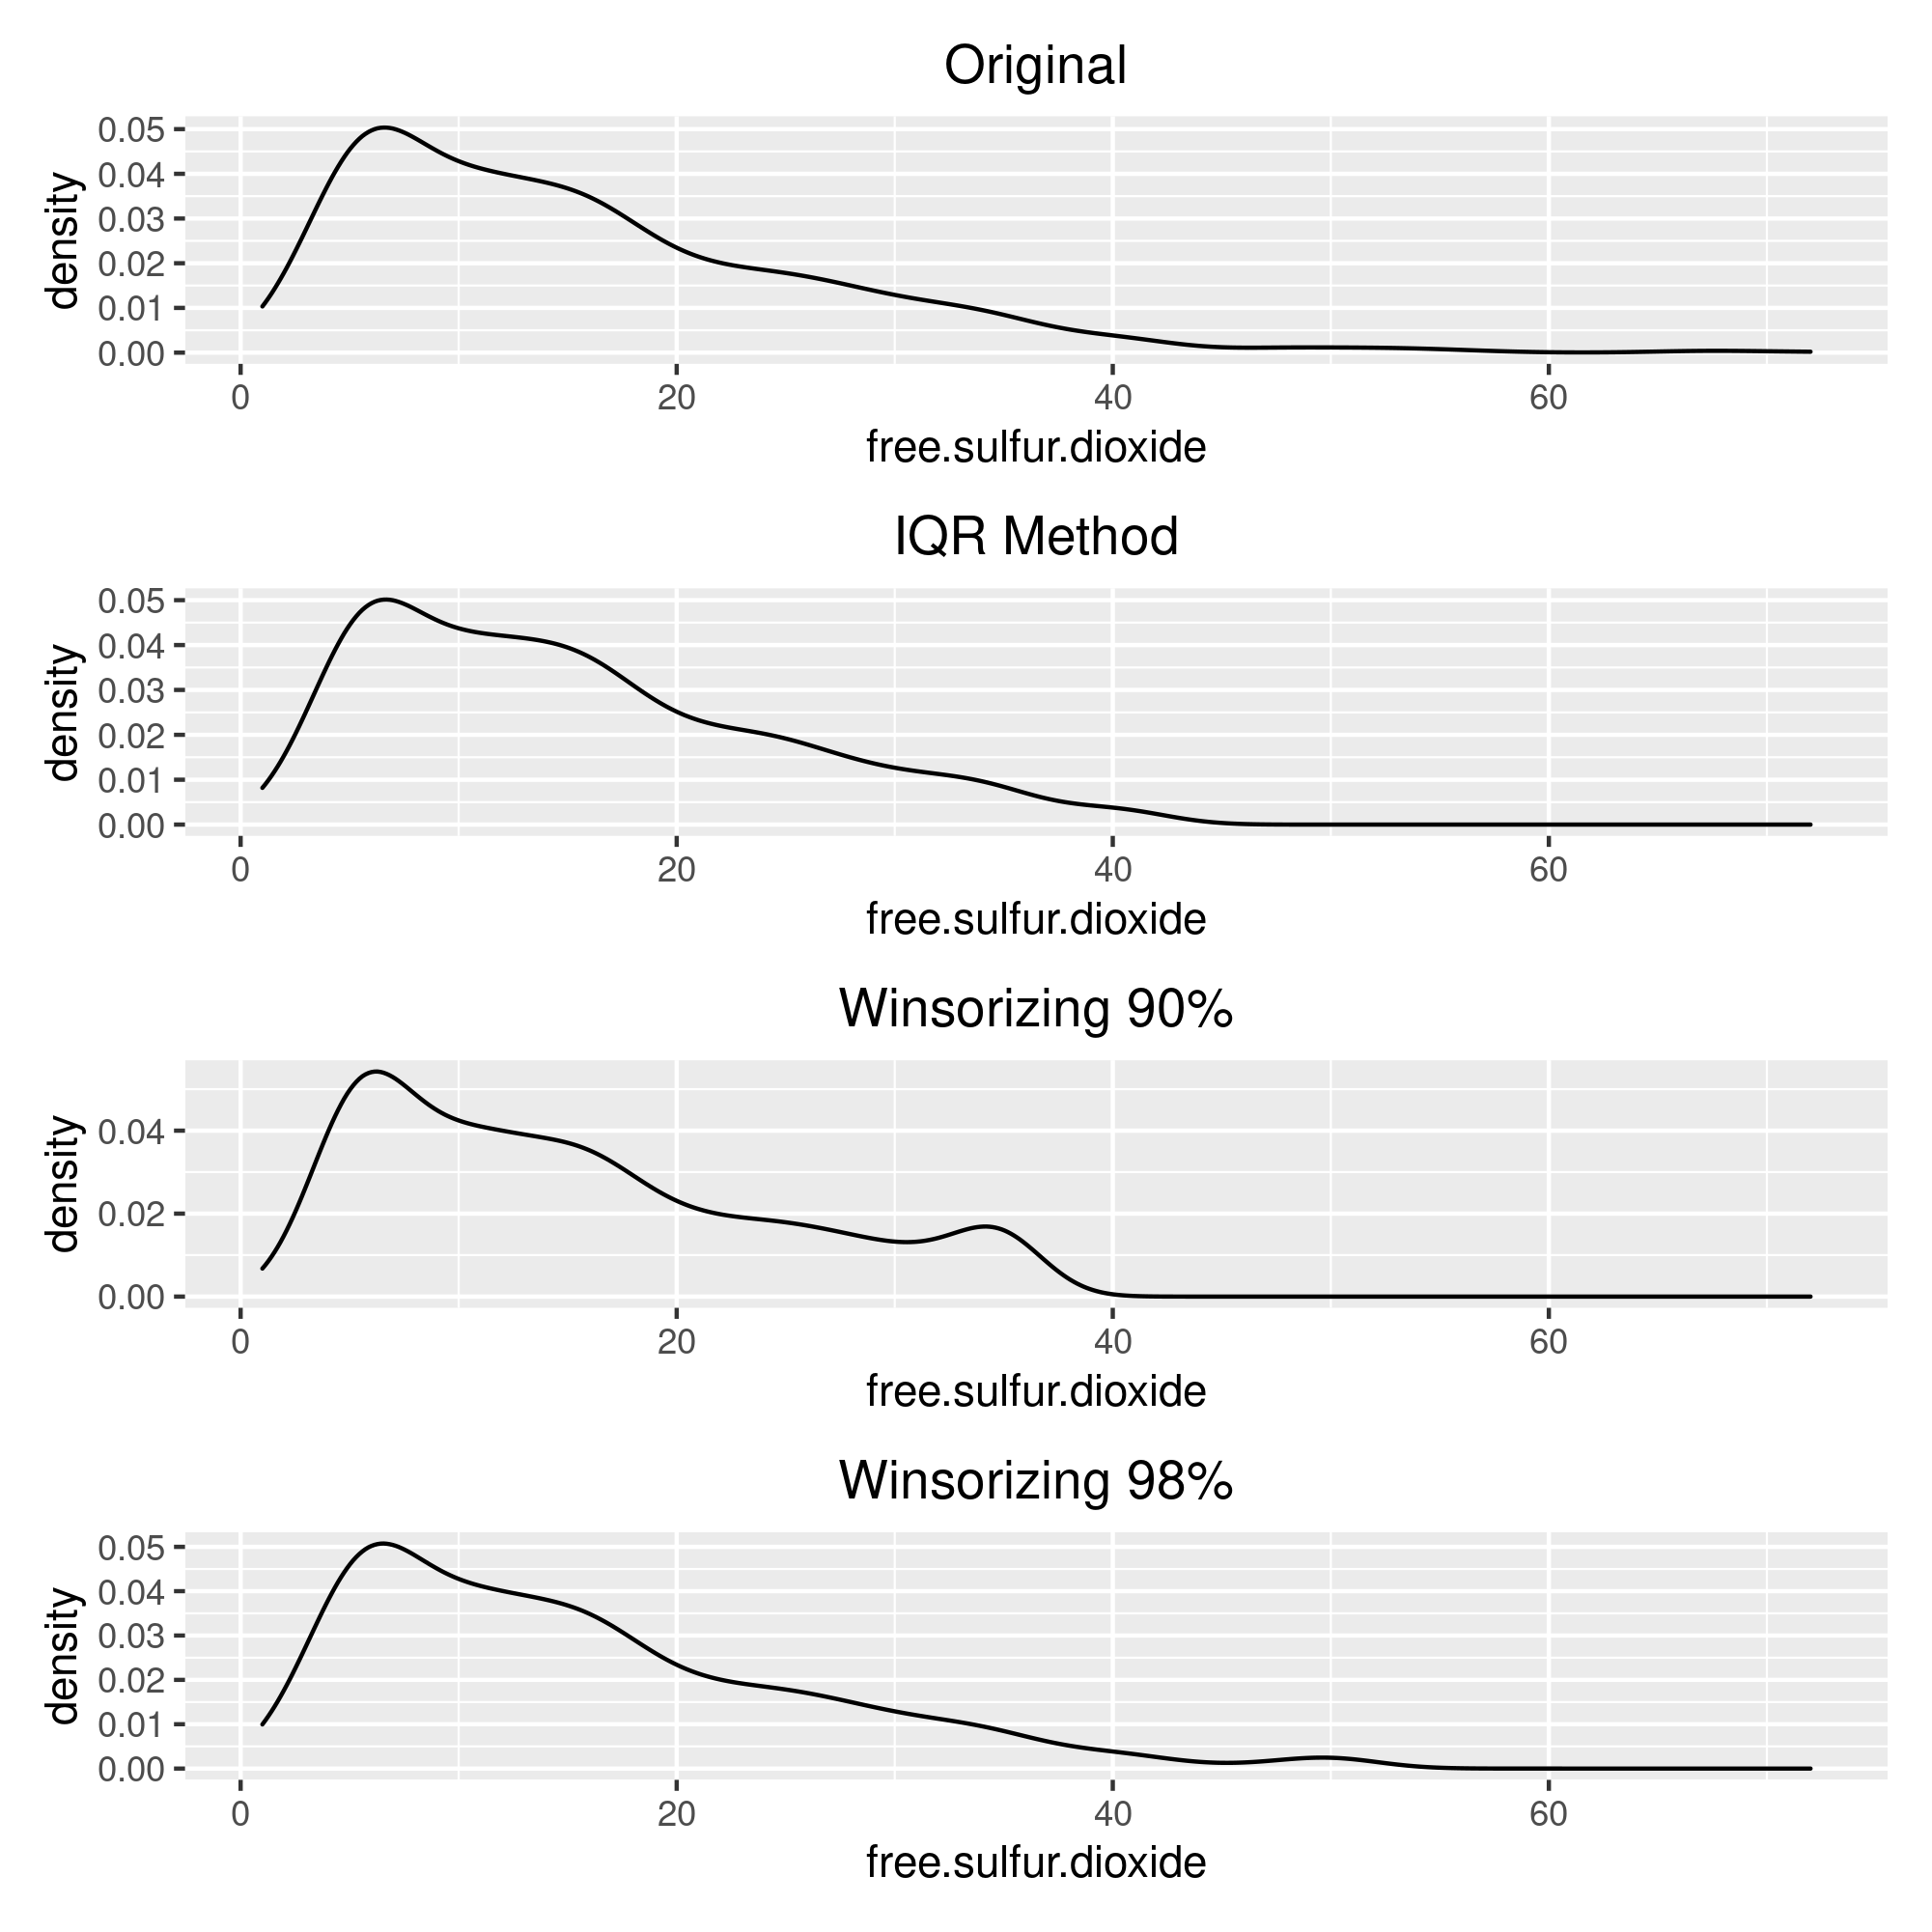
\includegraphics[width=0.45\textwidth]{images/outliers/free.sulfur.dioxide_distribution.png}
    }\qquad
    \subfloat[]{%
        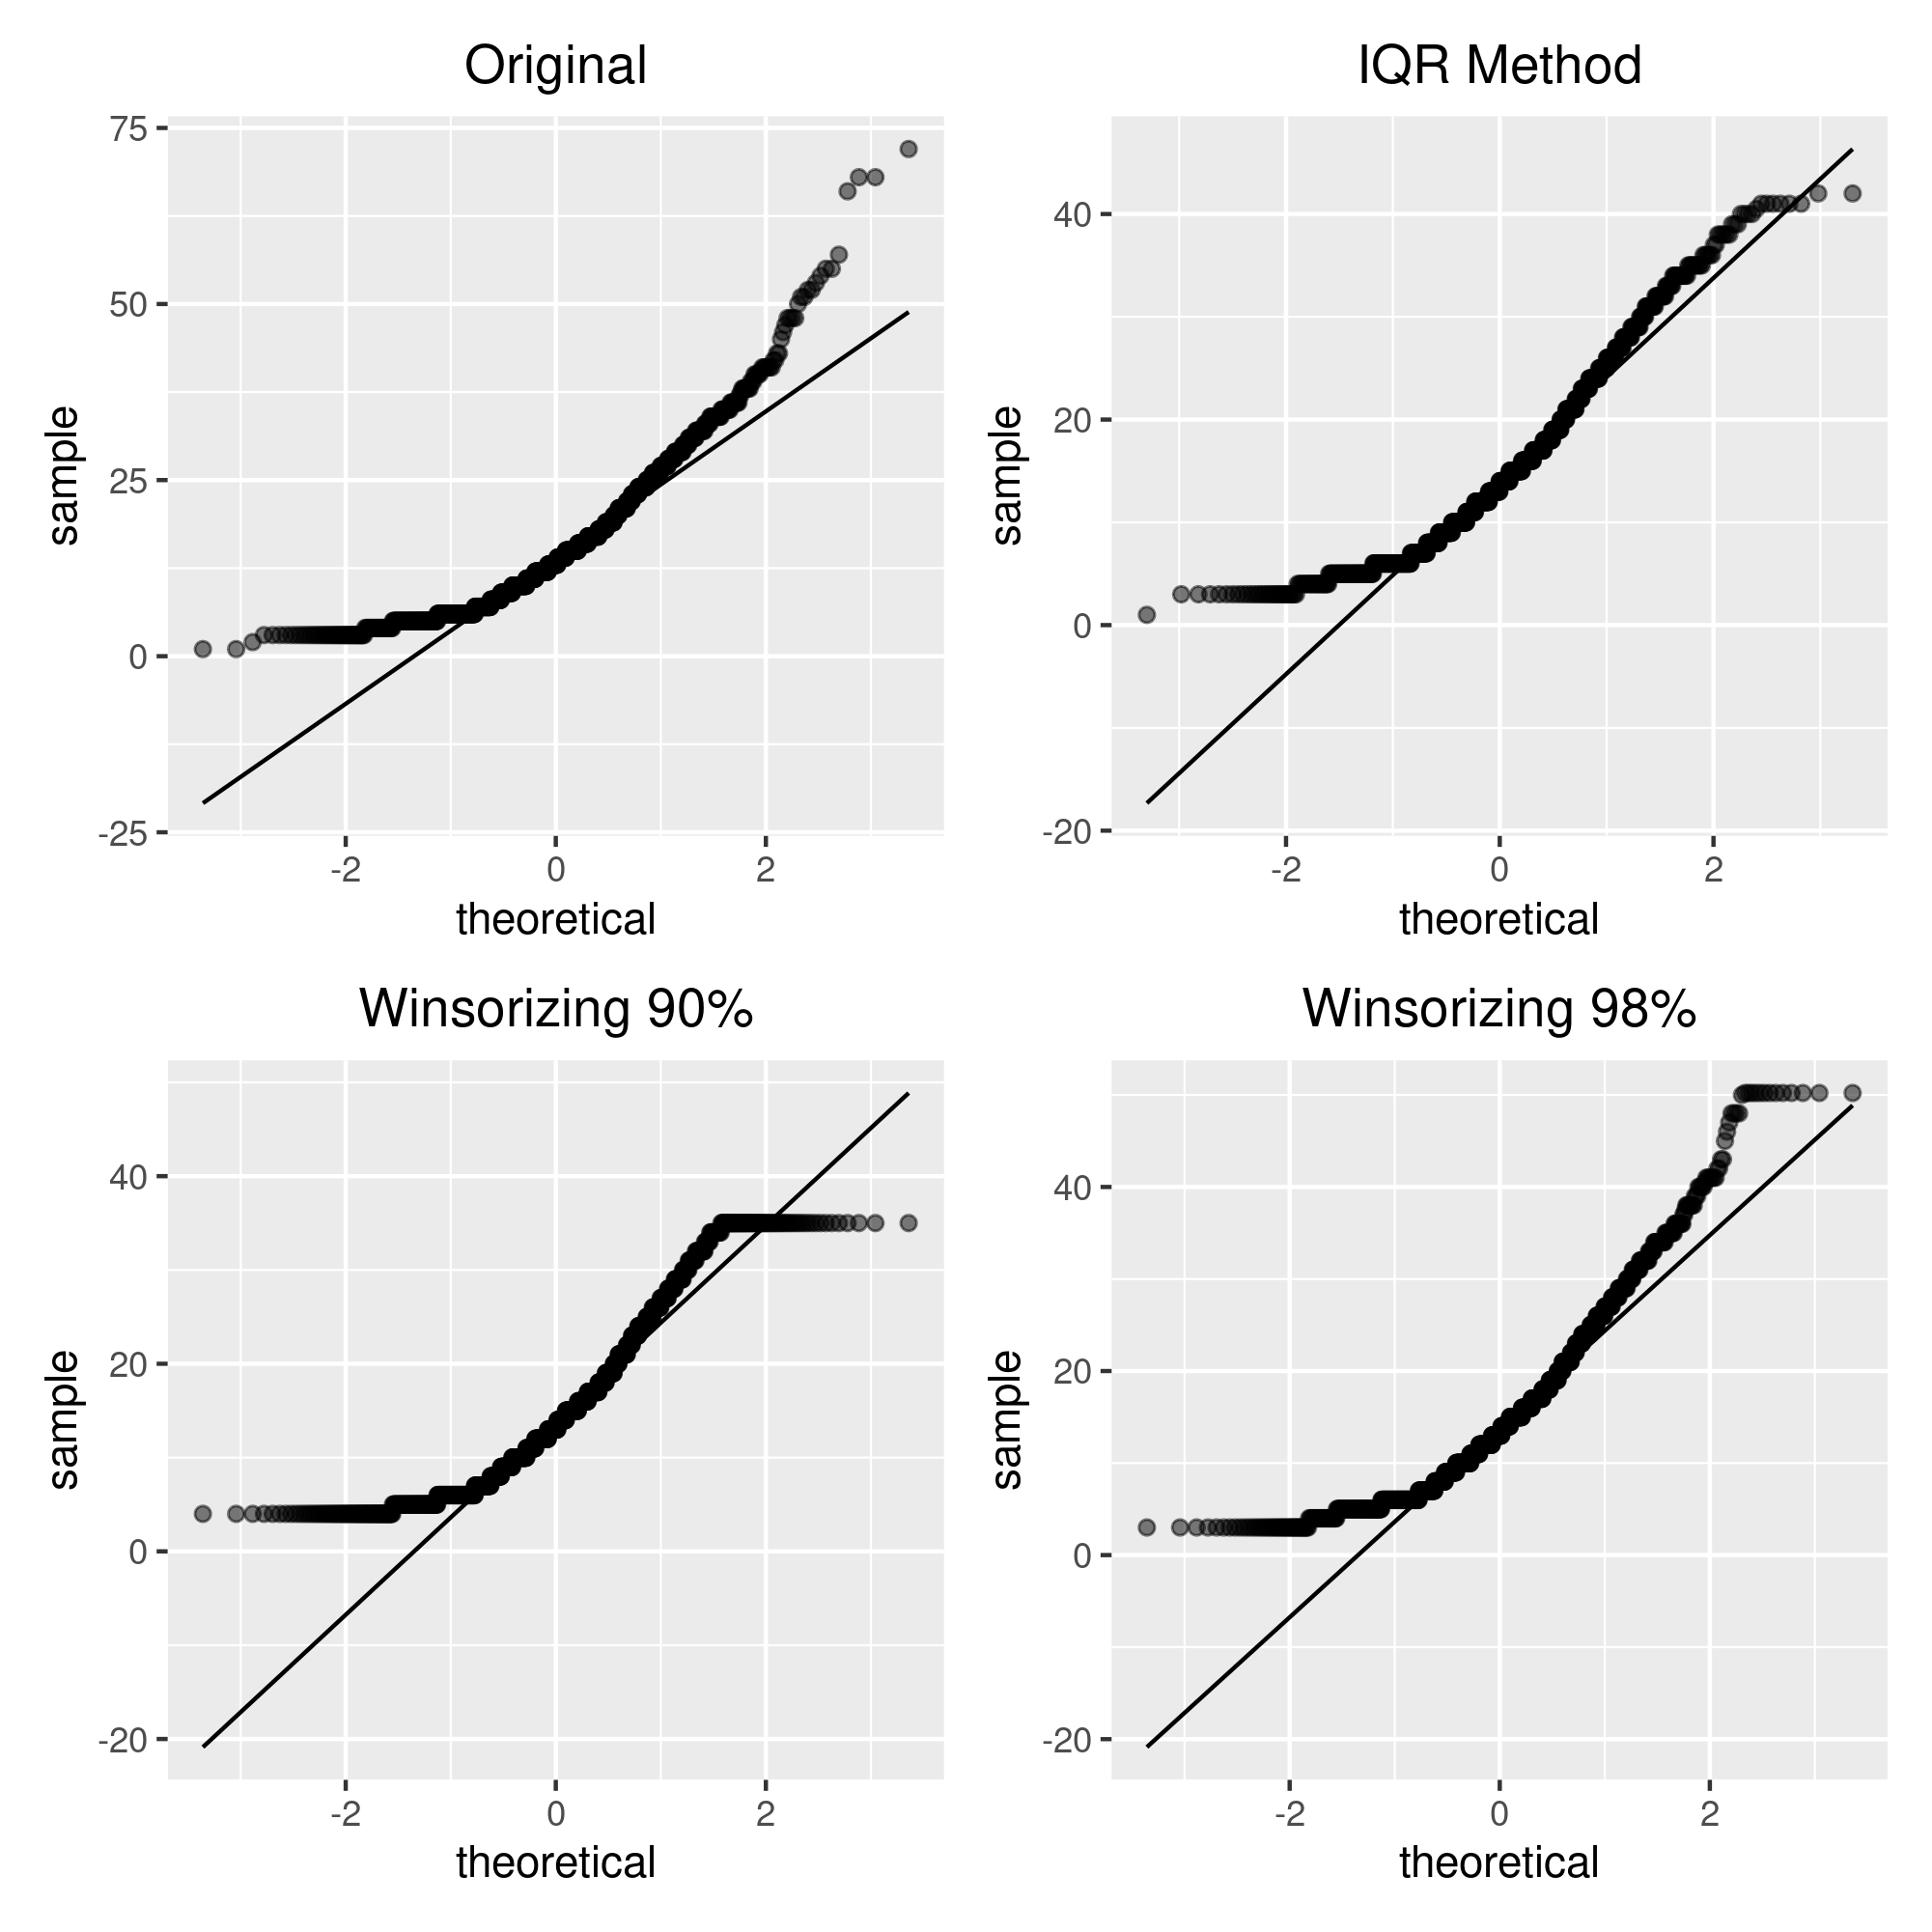
\includegraphics[width=0.45\textwidth]{images/outliers/free.sulfur.dioxide_qqplot.png}
    }

    \label{fig:free.sulfur.dioxide}
    \caption{Commento}
\end{figure}

\begin{figure}[H]
    \centering

    \subfloat[]{%
        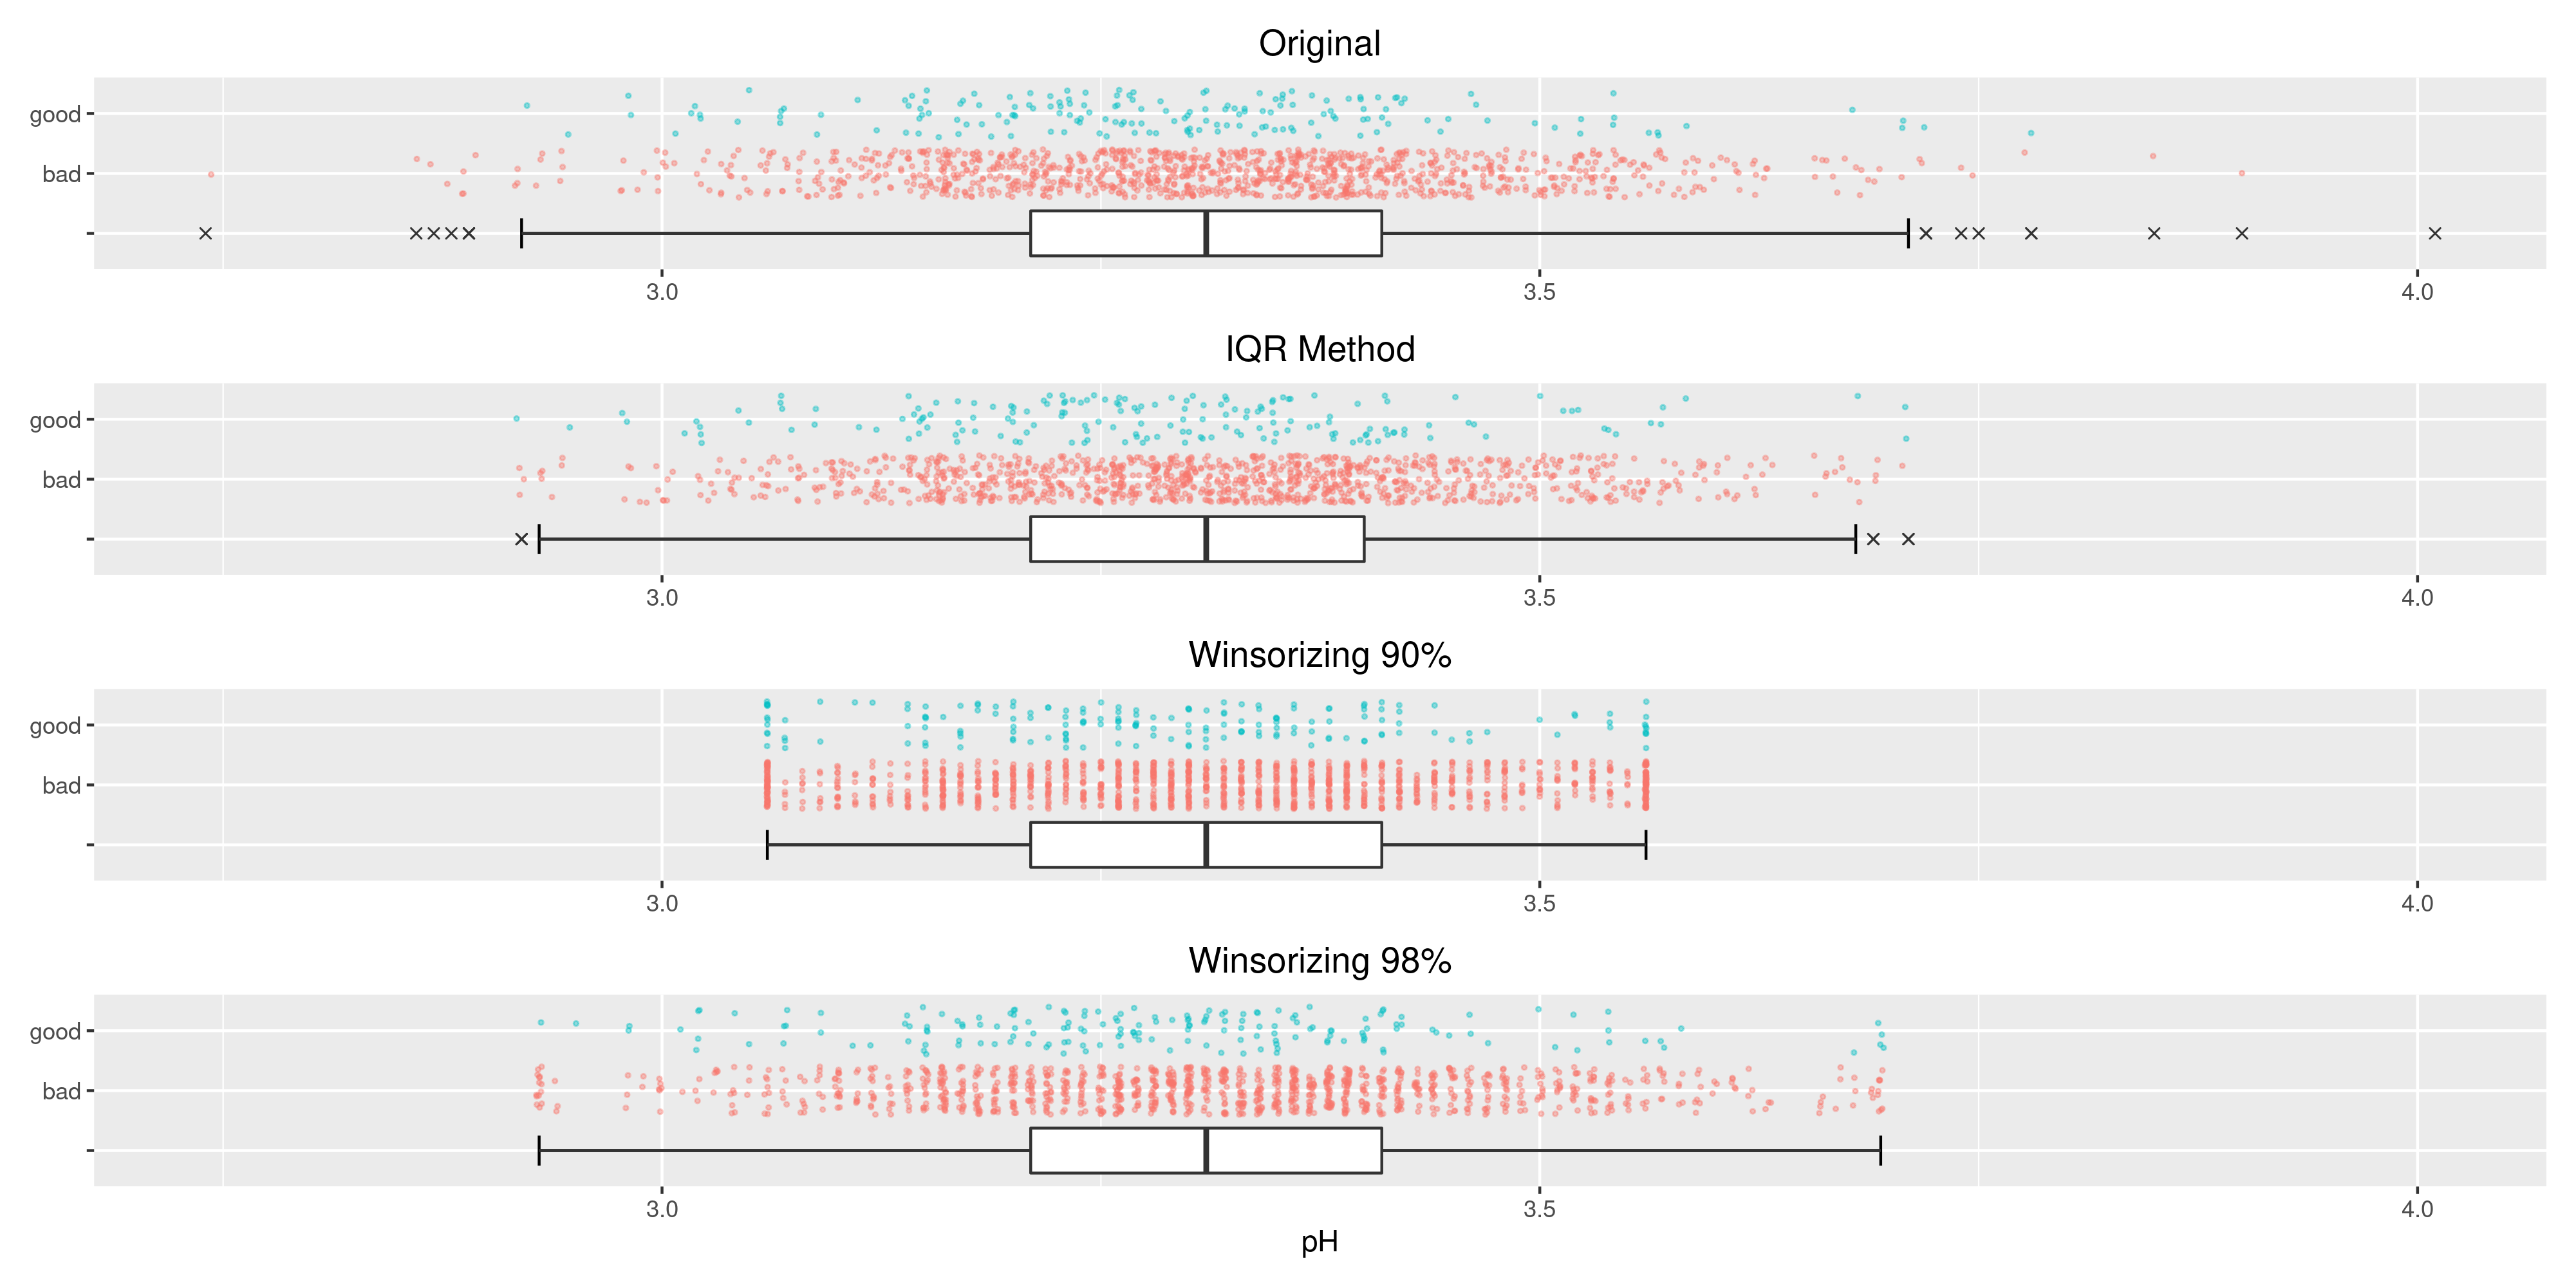
\includegraphics[width=0.99\textwidth]{images/outliers/pH_boxplot.png}
    }

    \subfloat[]{%
        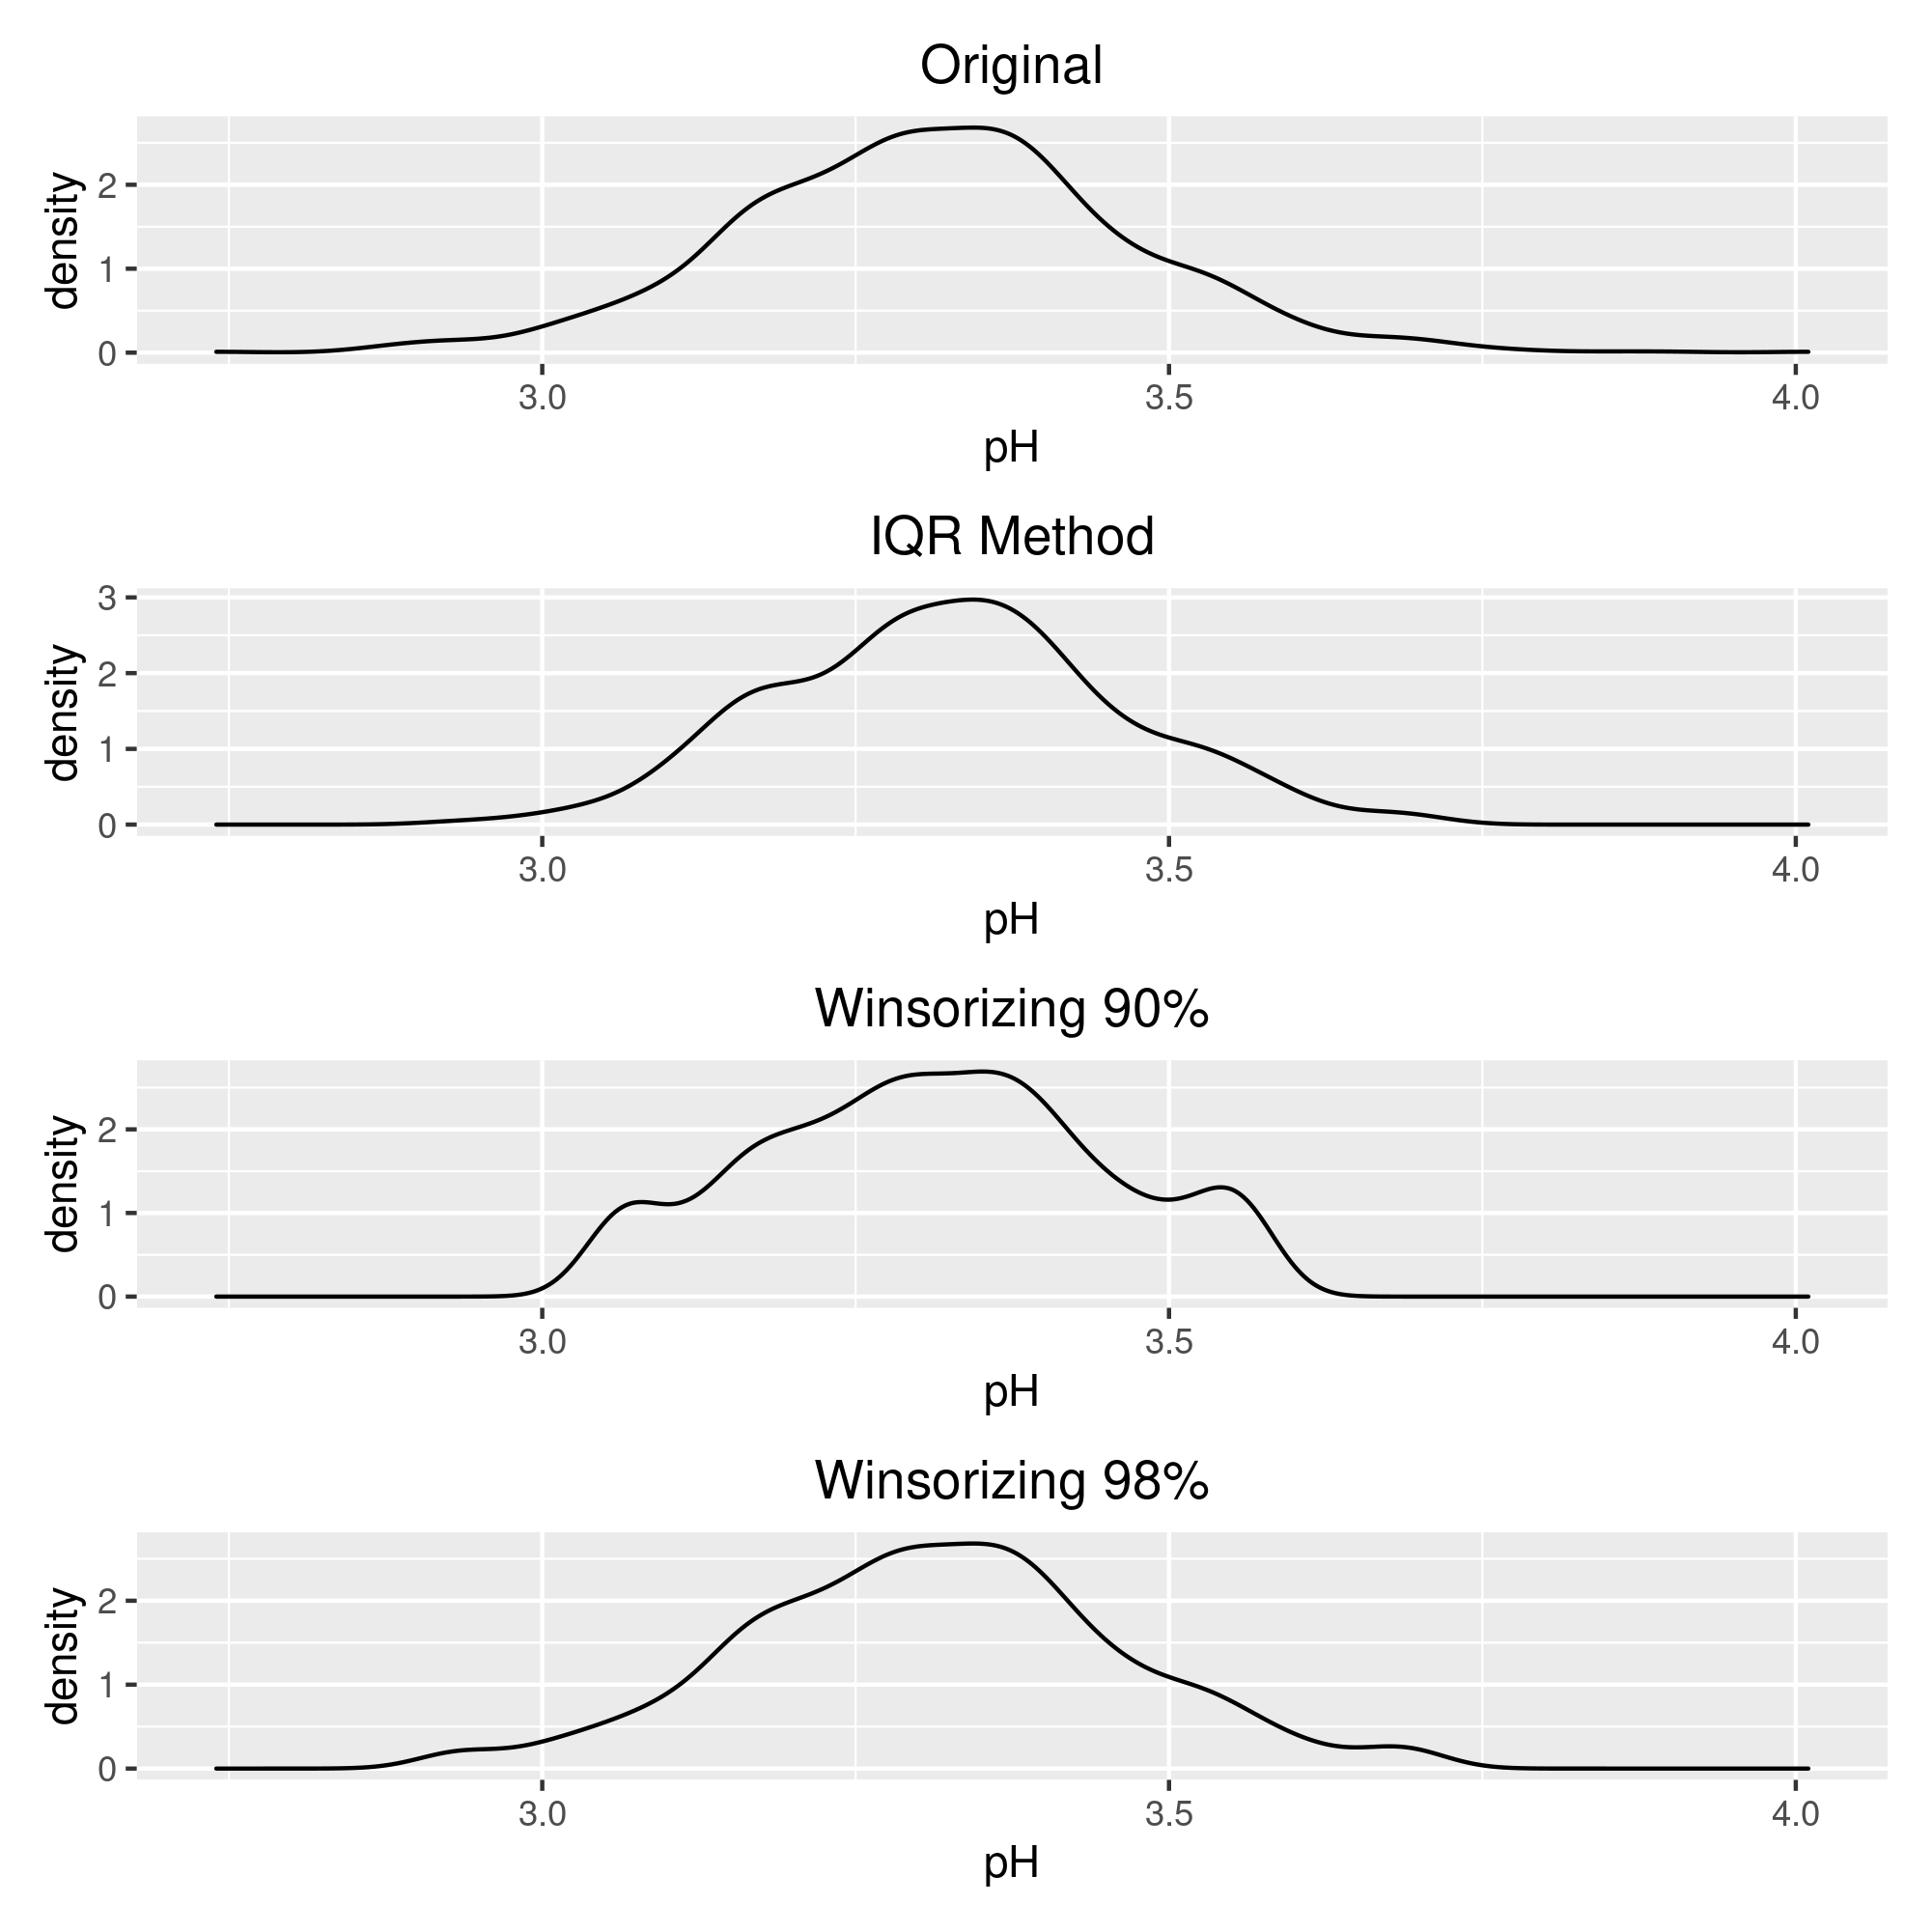
\includegraphics[width=0.45\textwidth]{images/outliers/pH_distribution.png}
    }\qquad
    \subfloat[]{%
        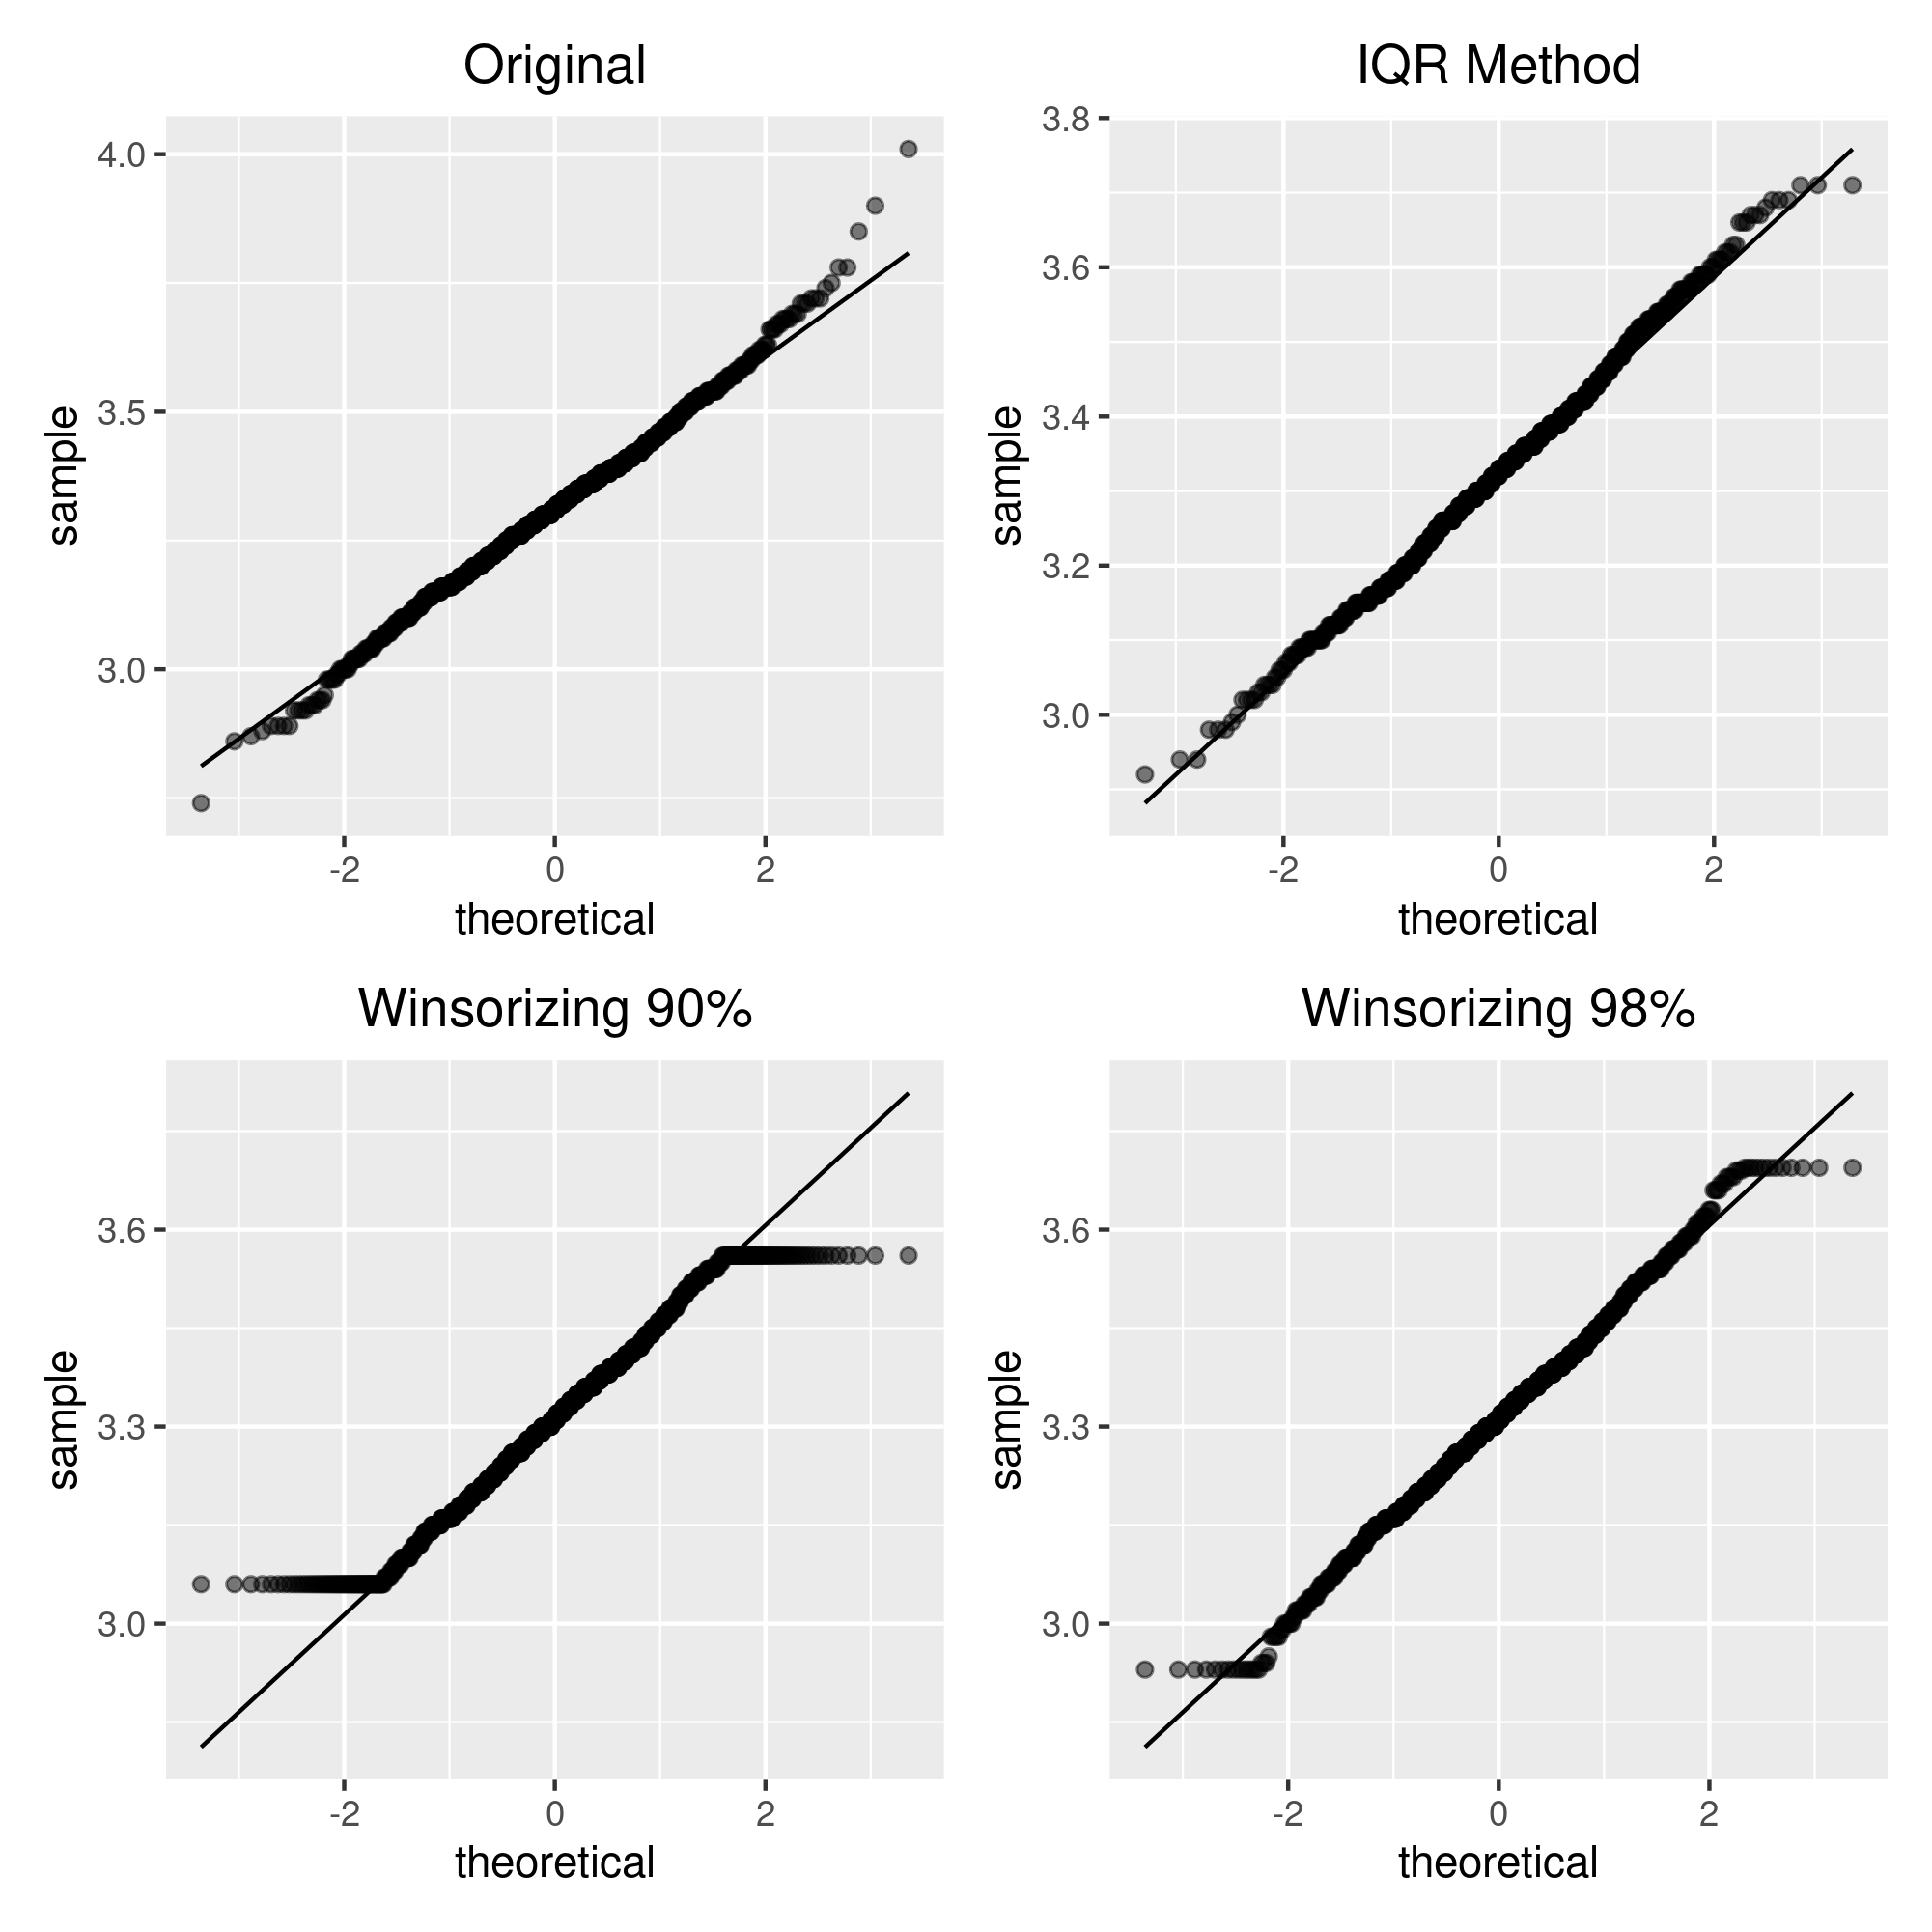
\includegraphics[width=0.45\textwidth]{images/outliers/pH_qqplot.png}
    }

    \label{fig:pH}
    \caption{Commento}
\end{figure}

\begin{figure}[H]
    \centering

    \subfloat[]{%
        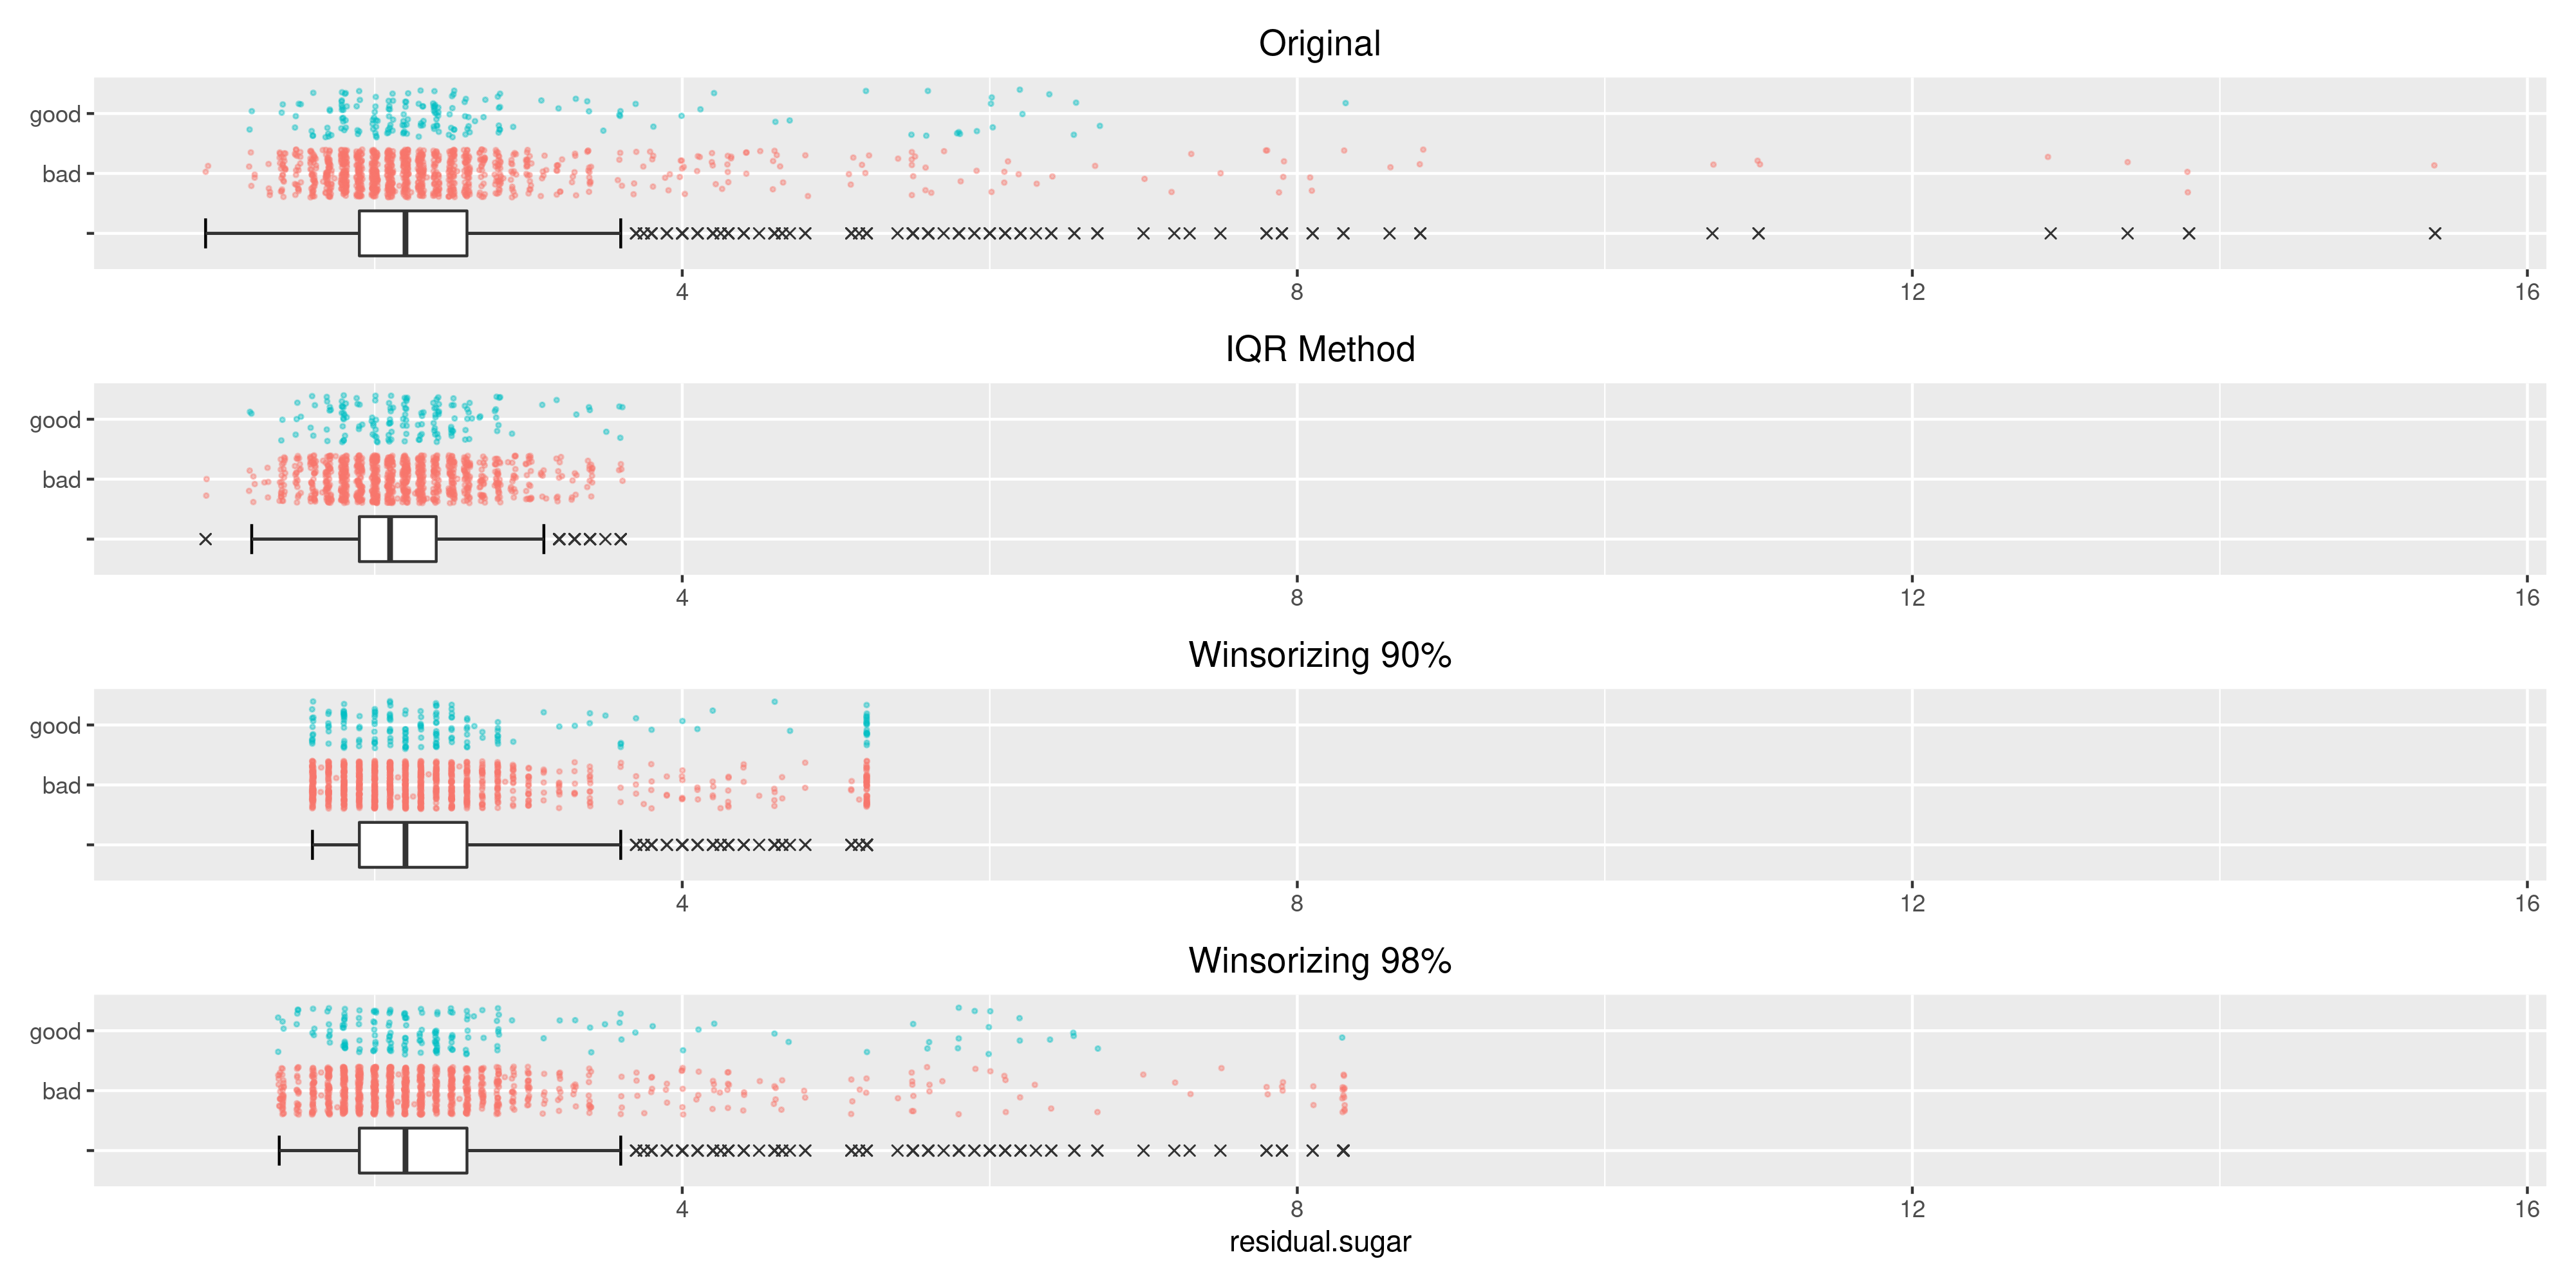
\includegraphics[width=0.99\textwidth]{images/outliers/residual.sugar_boxplot.png}
    }

    \subfloat[]{%
        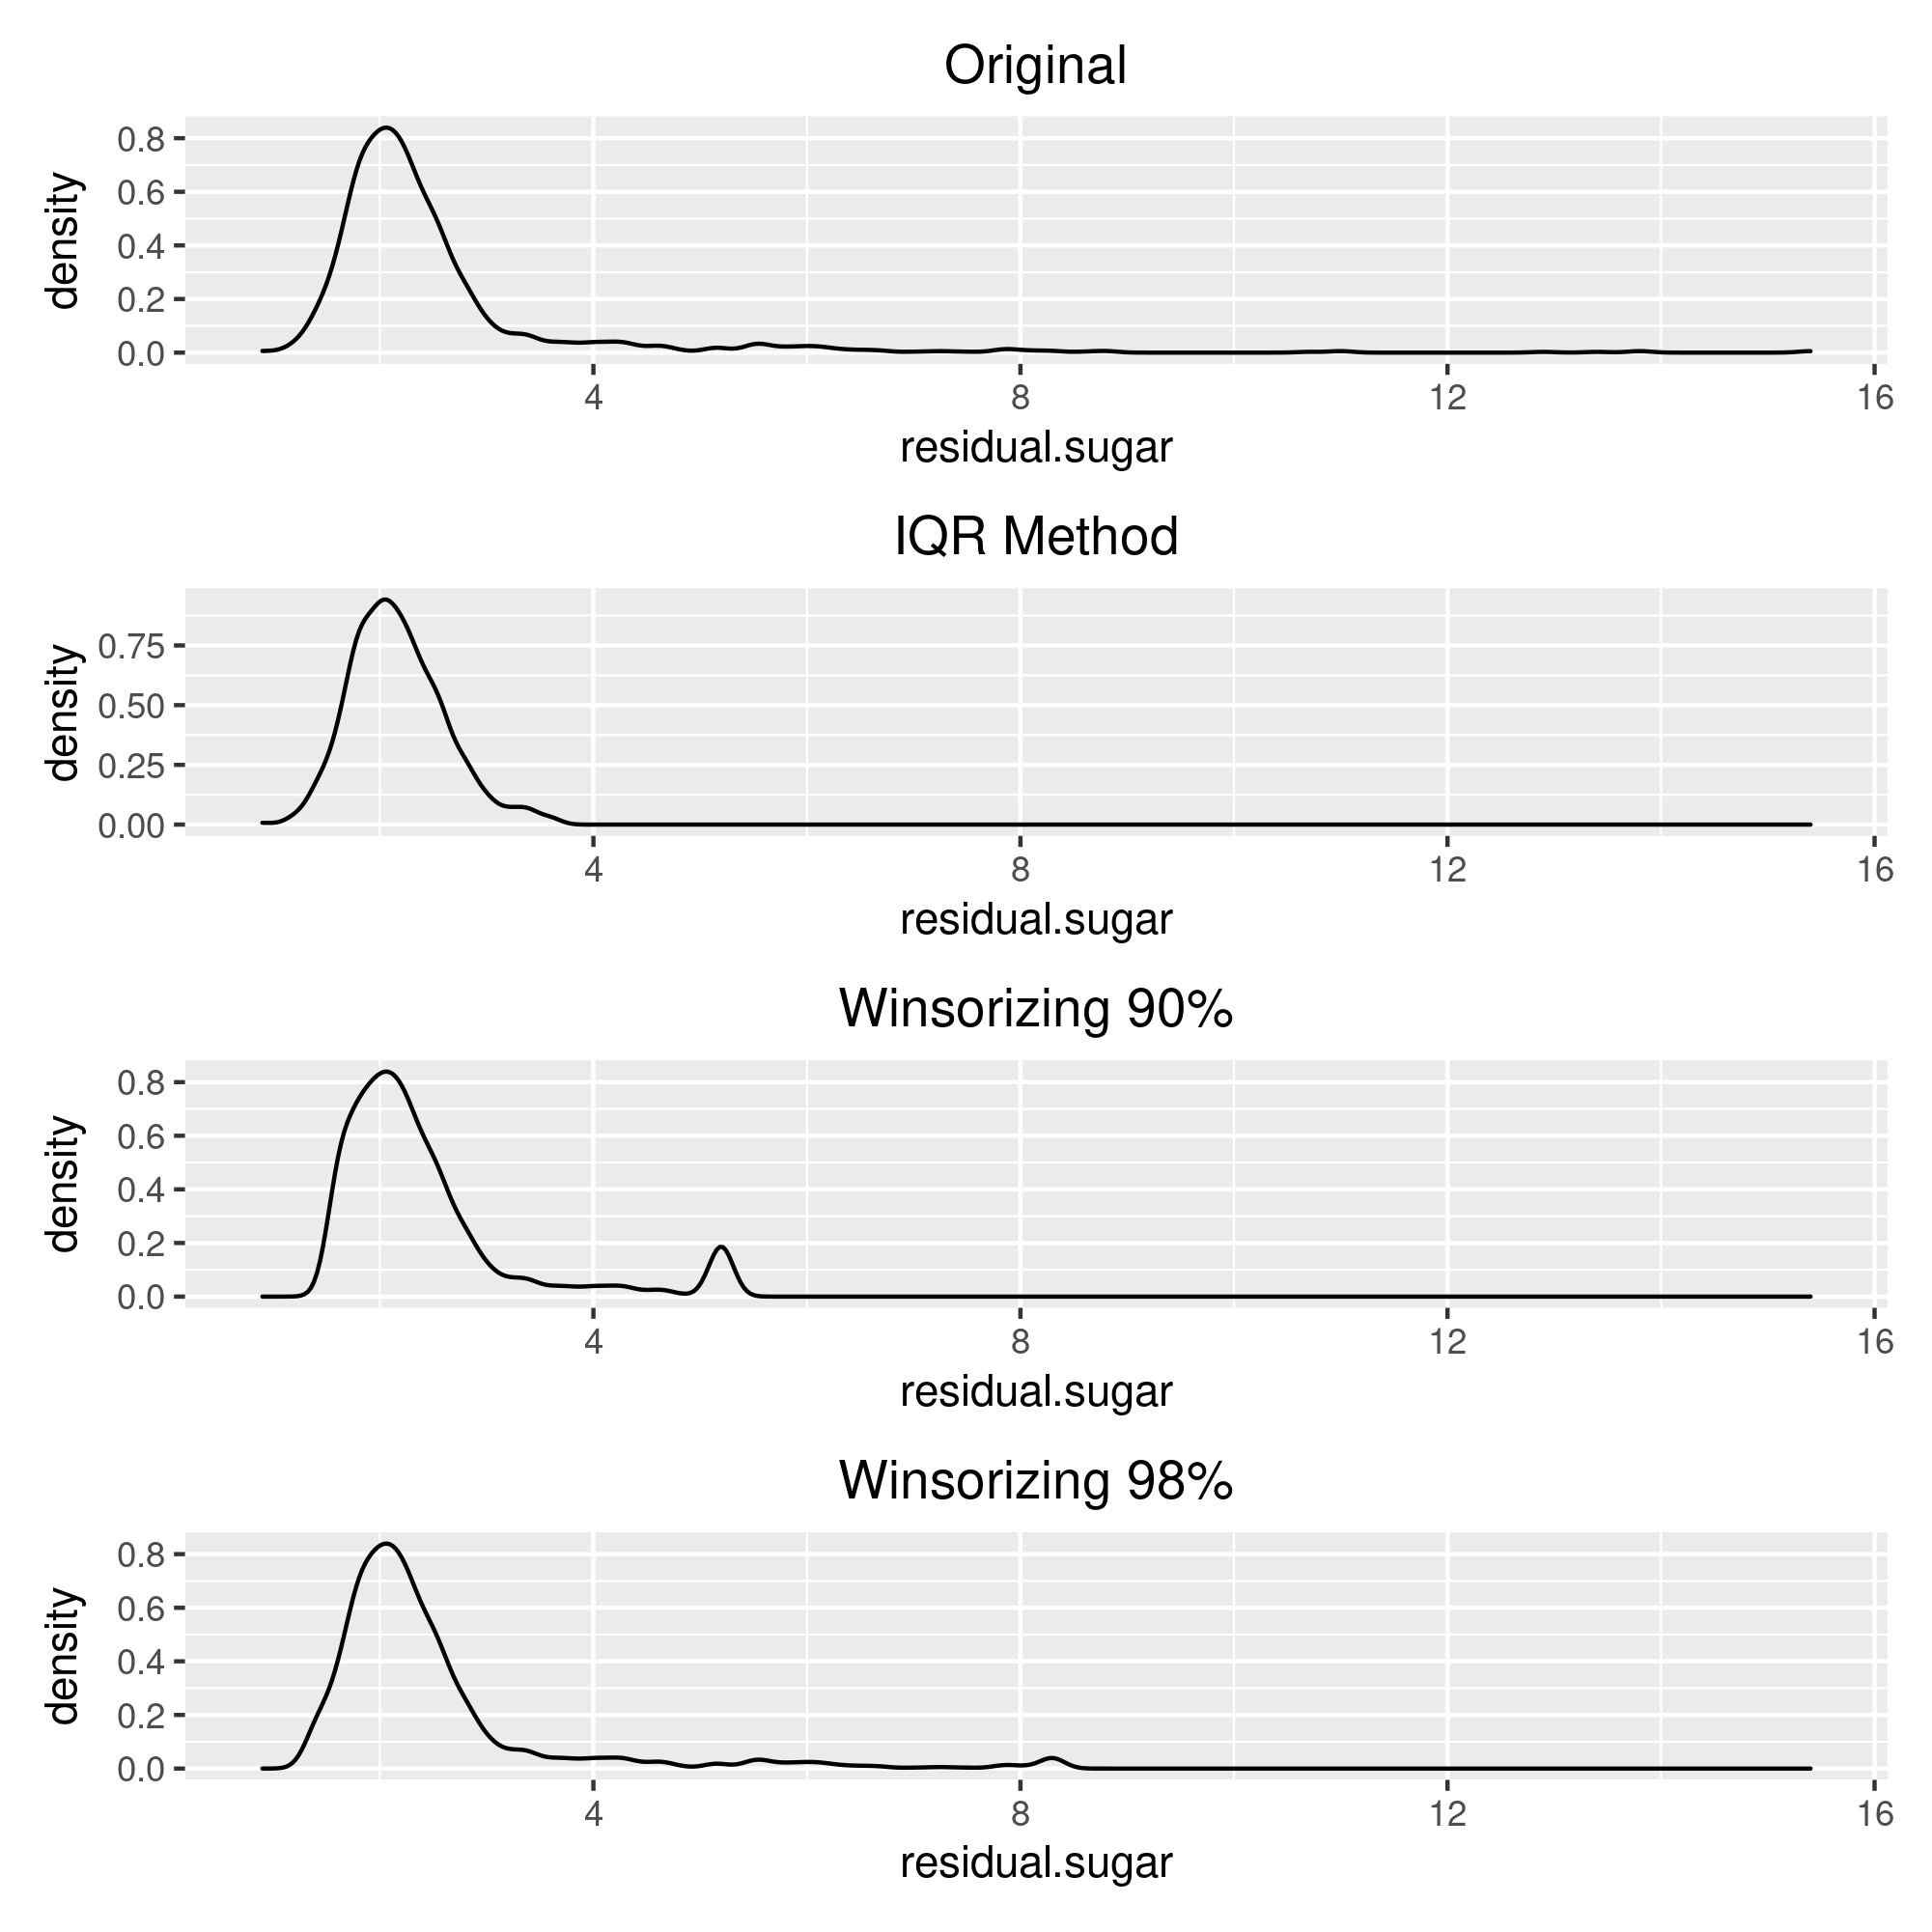
\includegraphics[width=0.45\textwidth]{images/outliers/residual.sugar_distribution.png}
    }\qquad
    \subfloat[]{%
        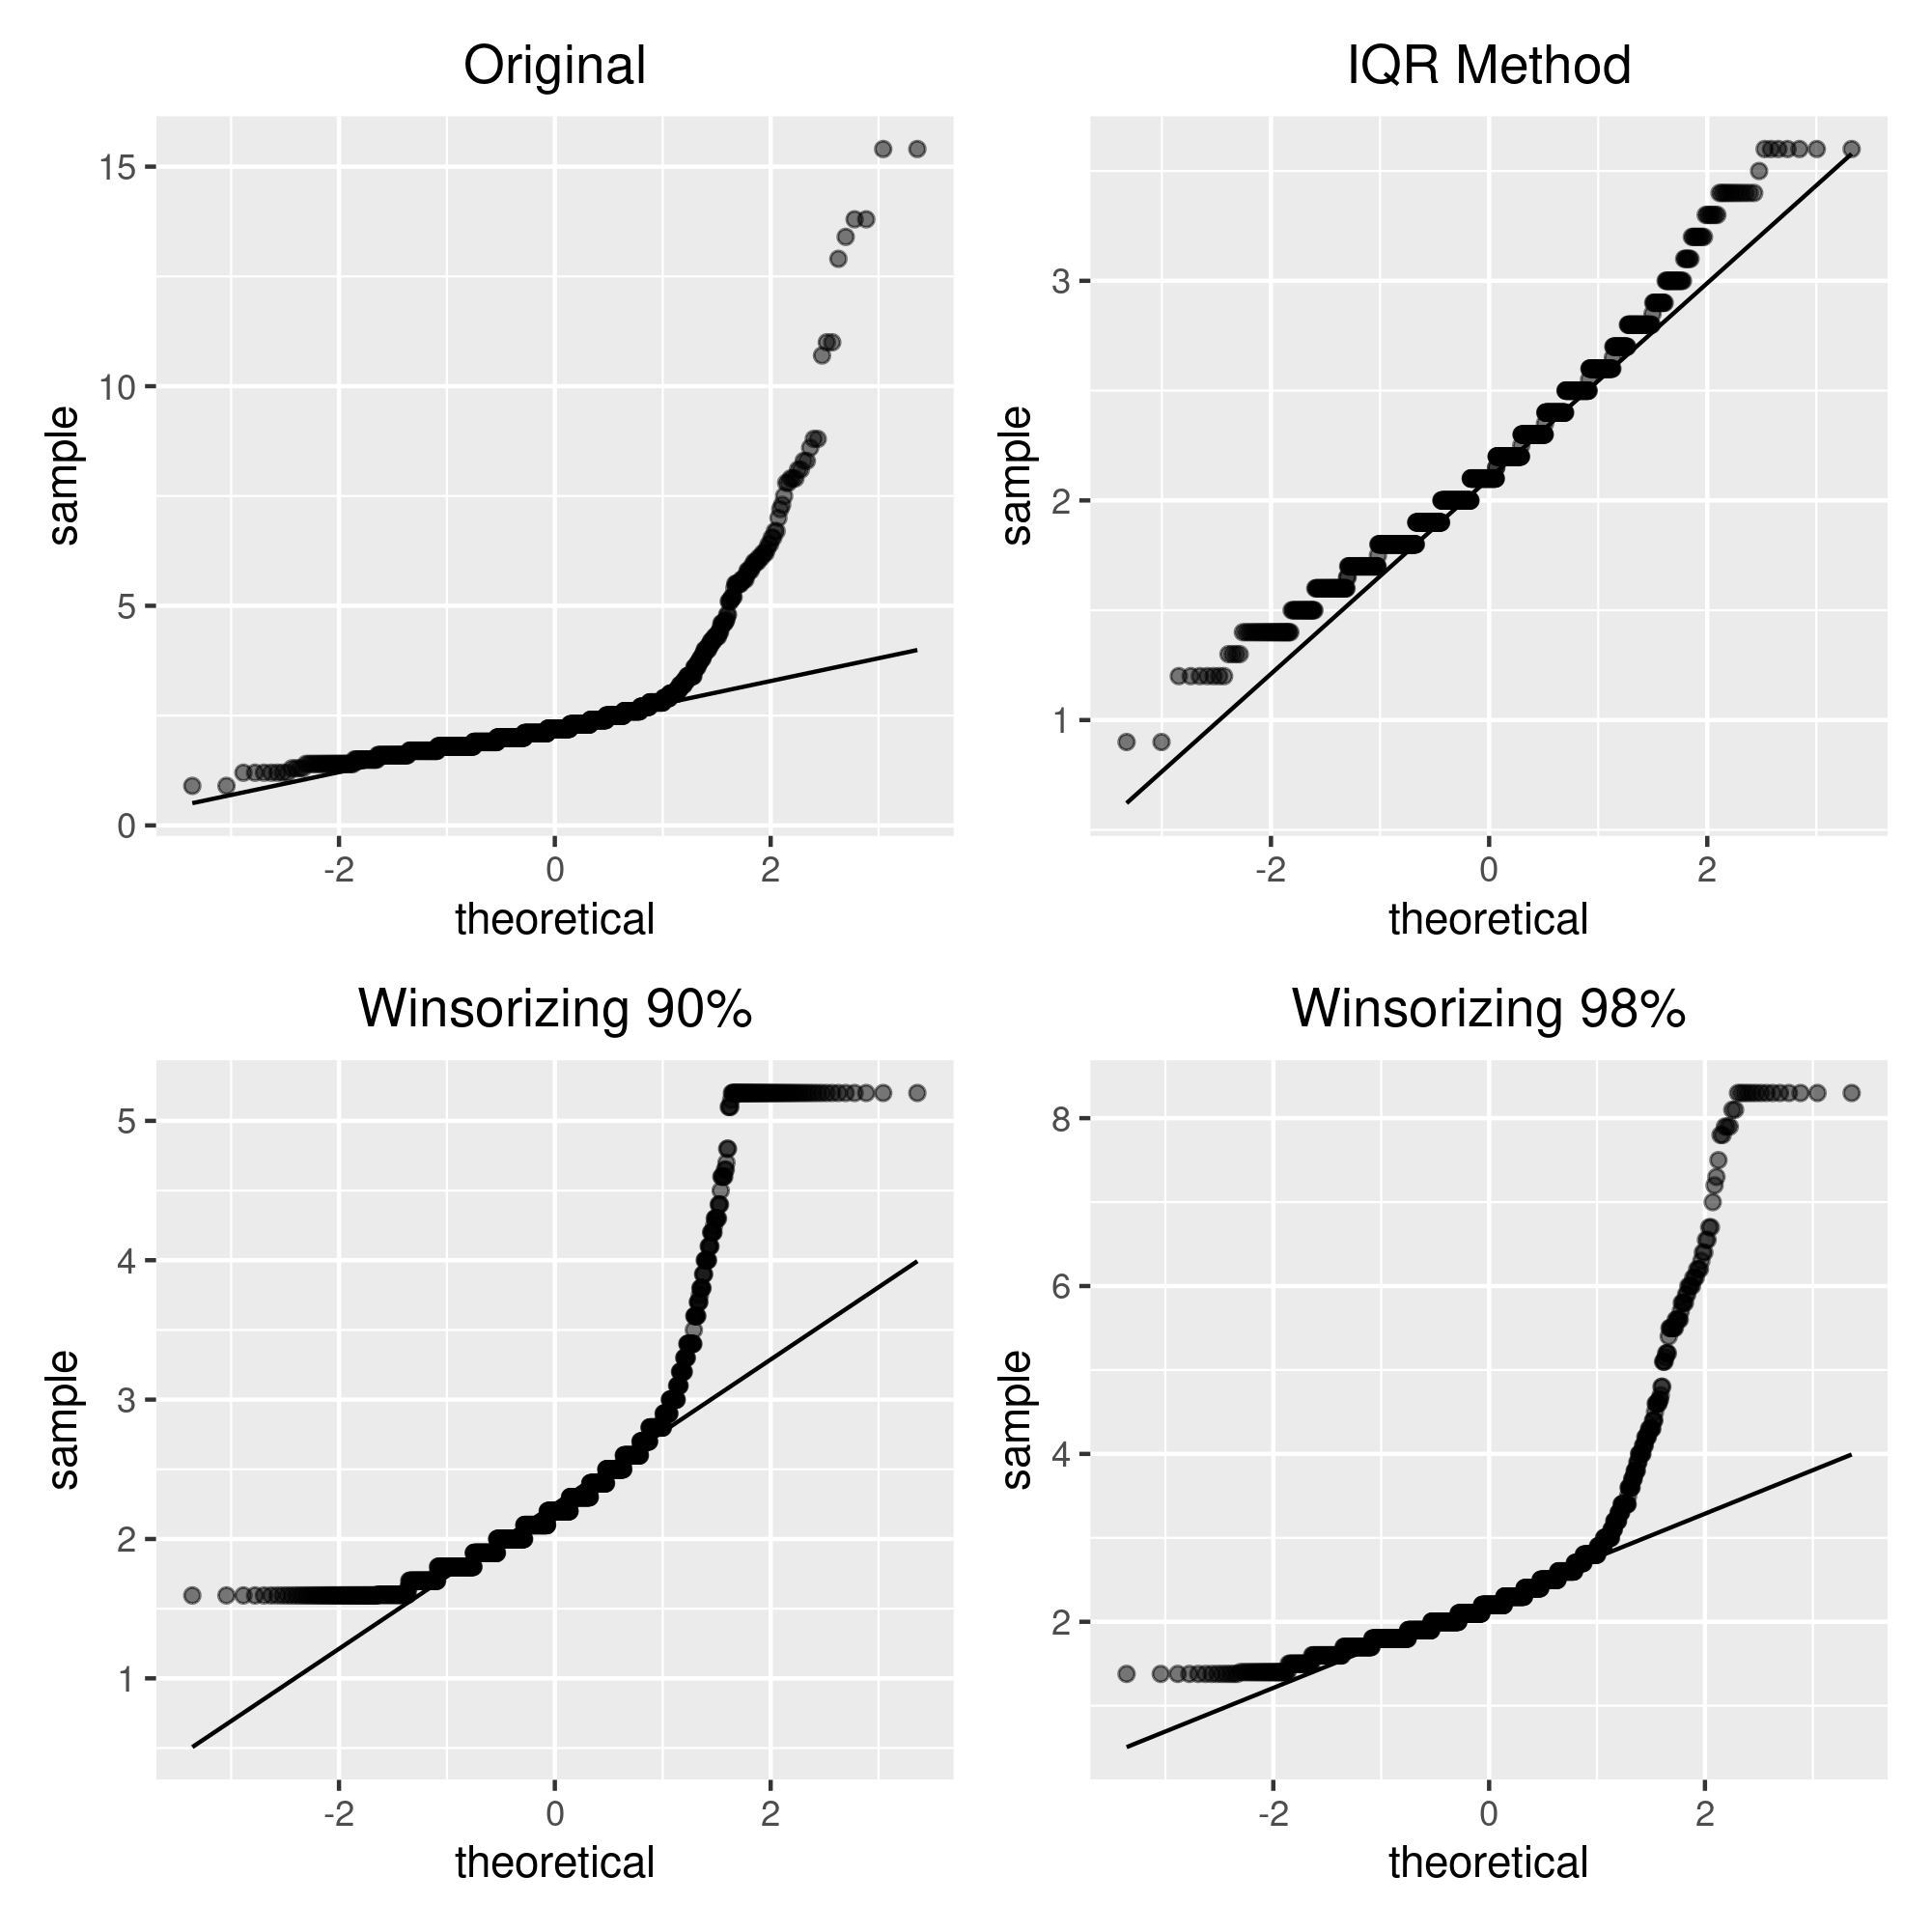
\includegraphics[width=0.45\textwidth]{images/outliers/residual.sugar_qqplot.png}
    }

    \label{fig:residual.sugar}
    \caption{Commento}
\end{figure}

\begin{figure}[H]
    \centering

    \subfloat[]{%
        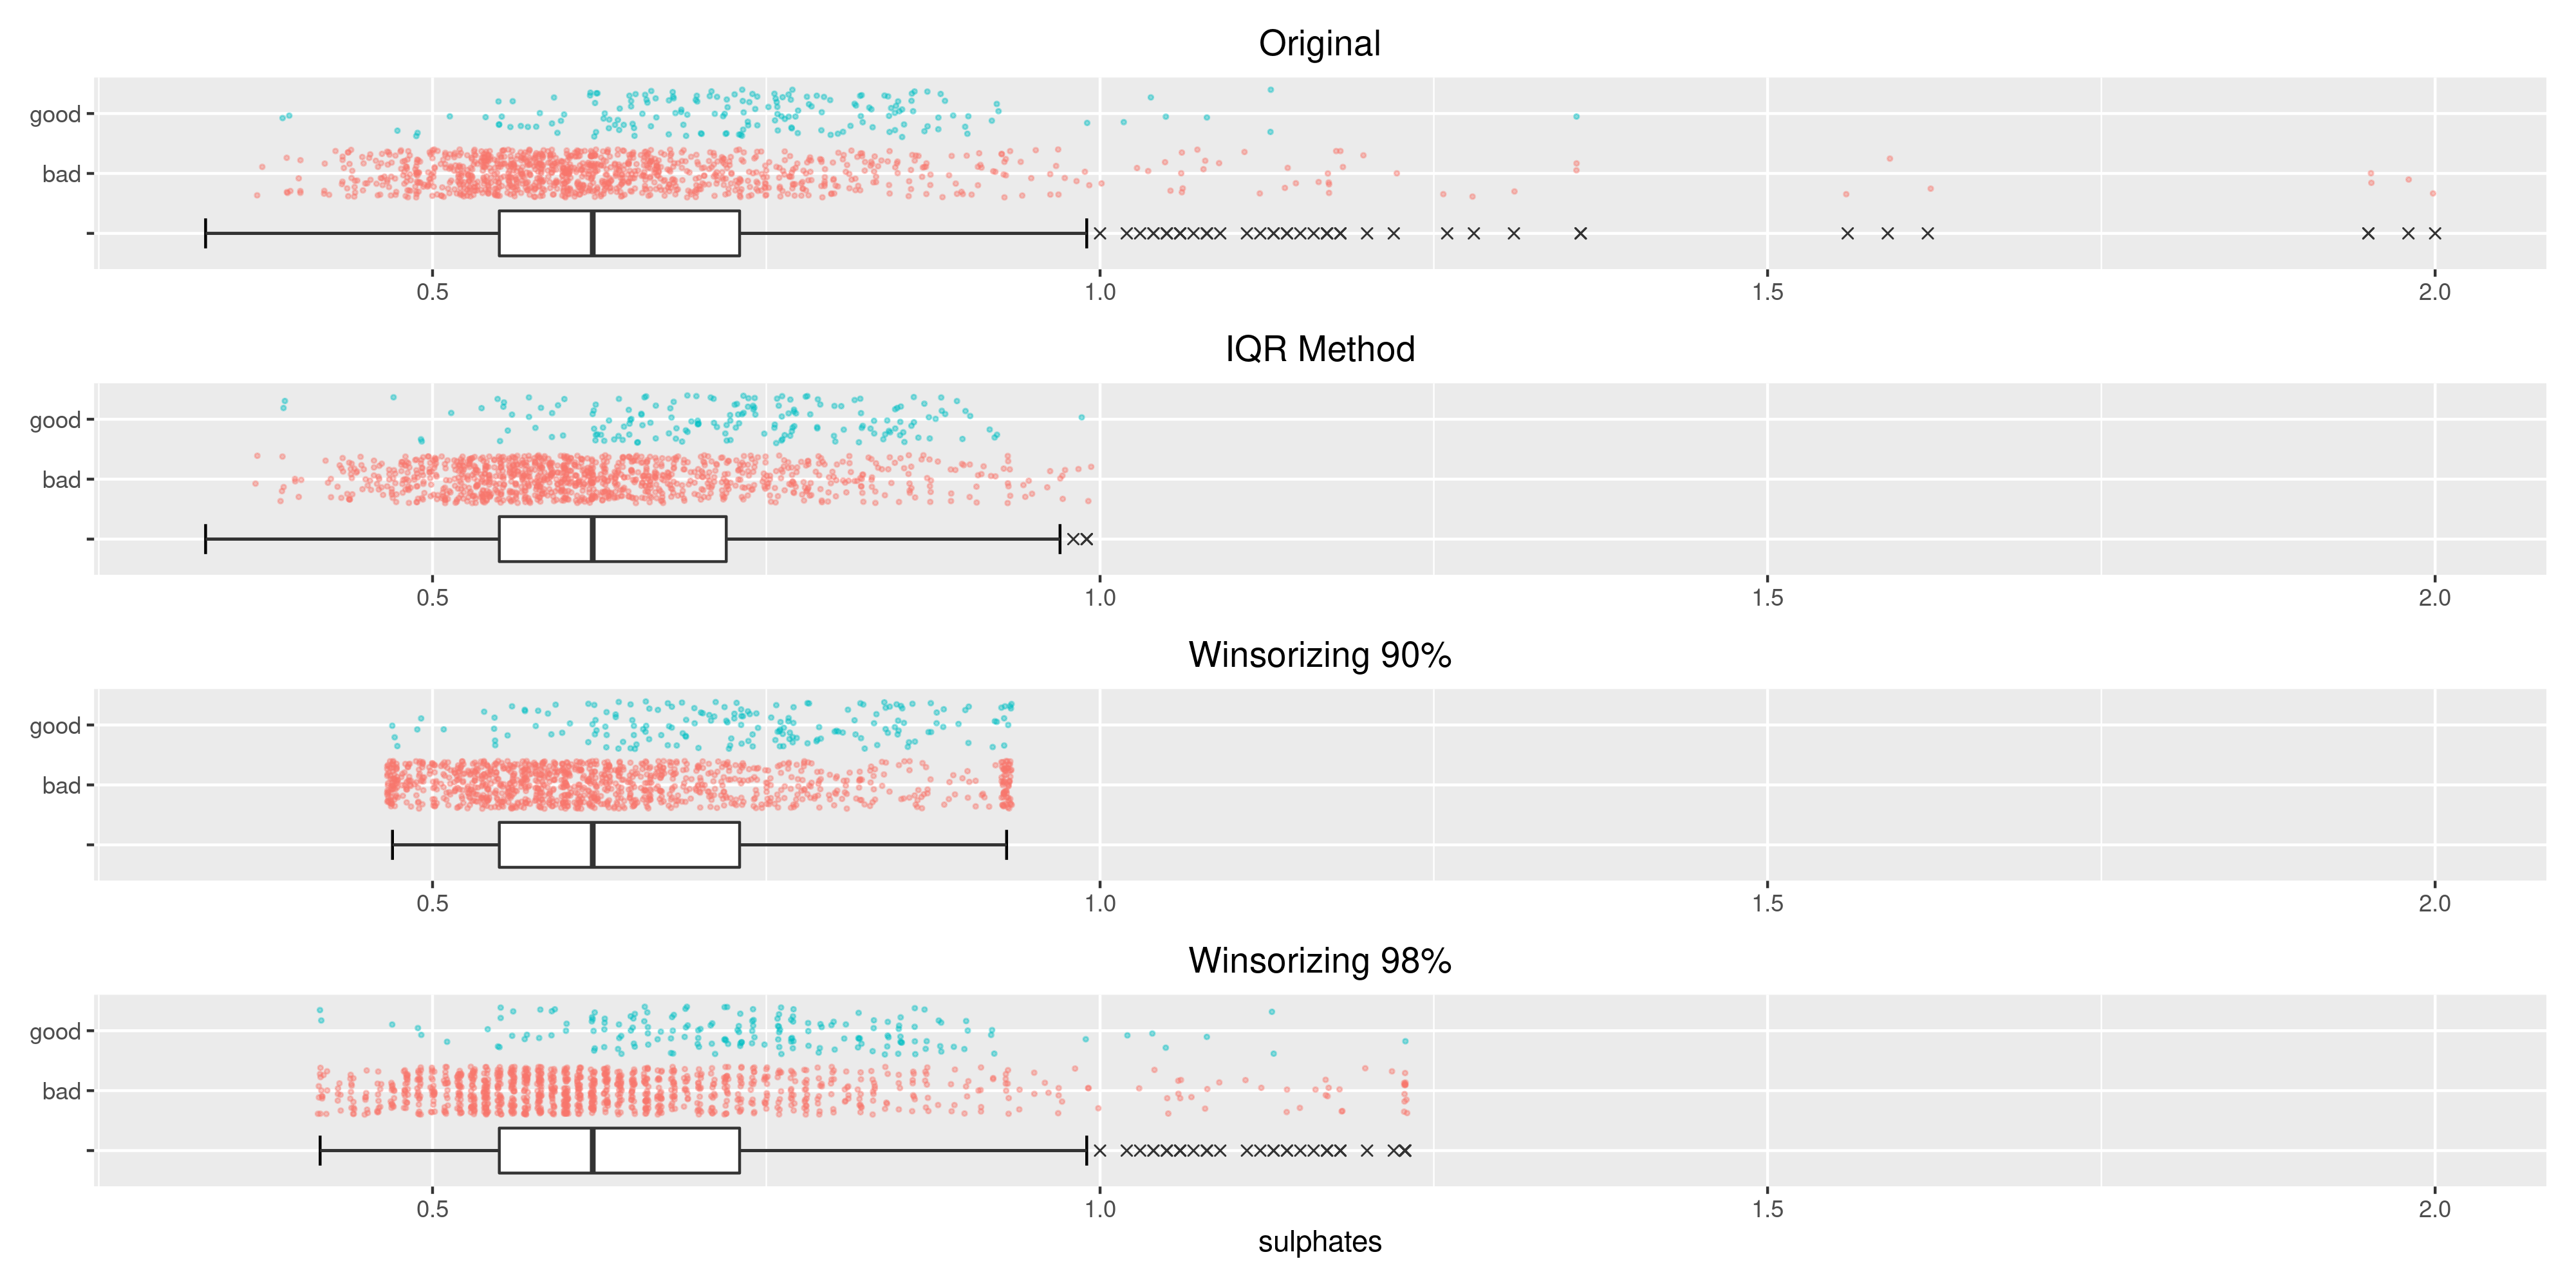
\includegraphics[width=0.99\textwidth]{images/outliers/sulphates_boxplot.png}
    }

    \subfloat[]{%
        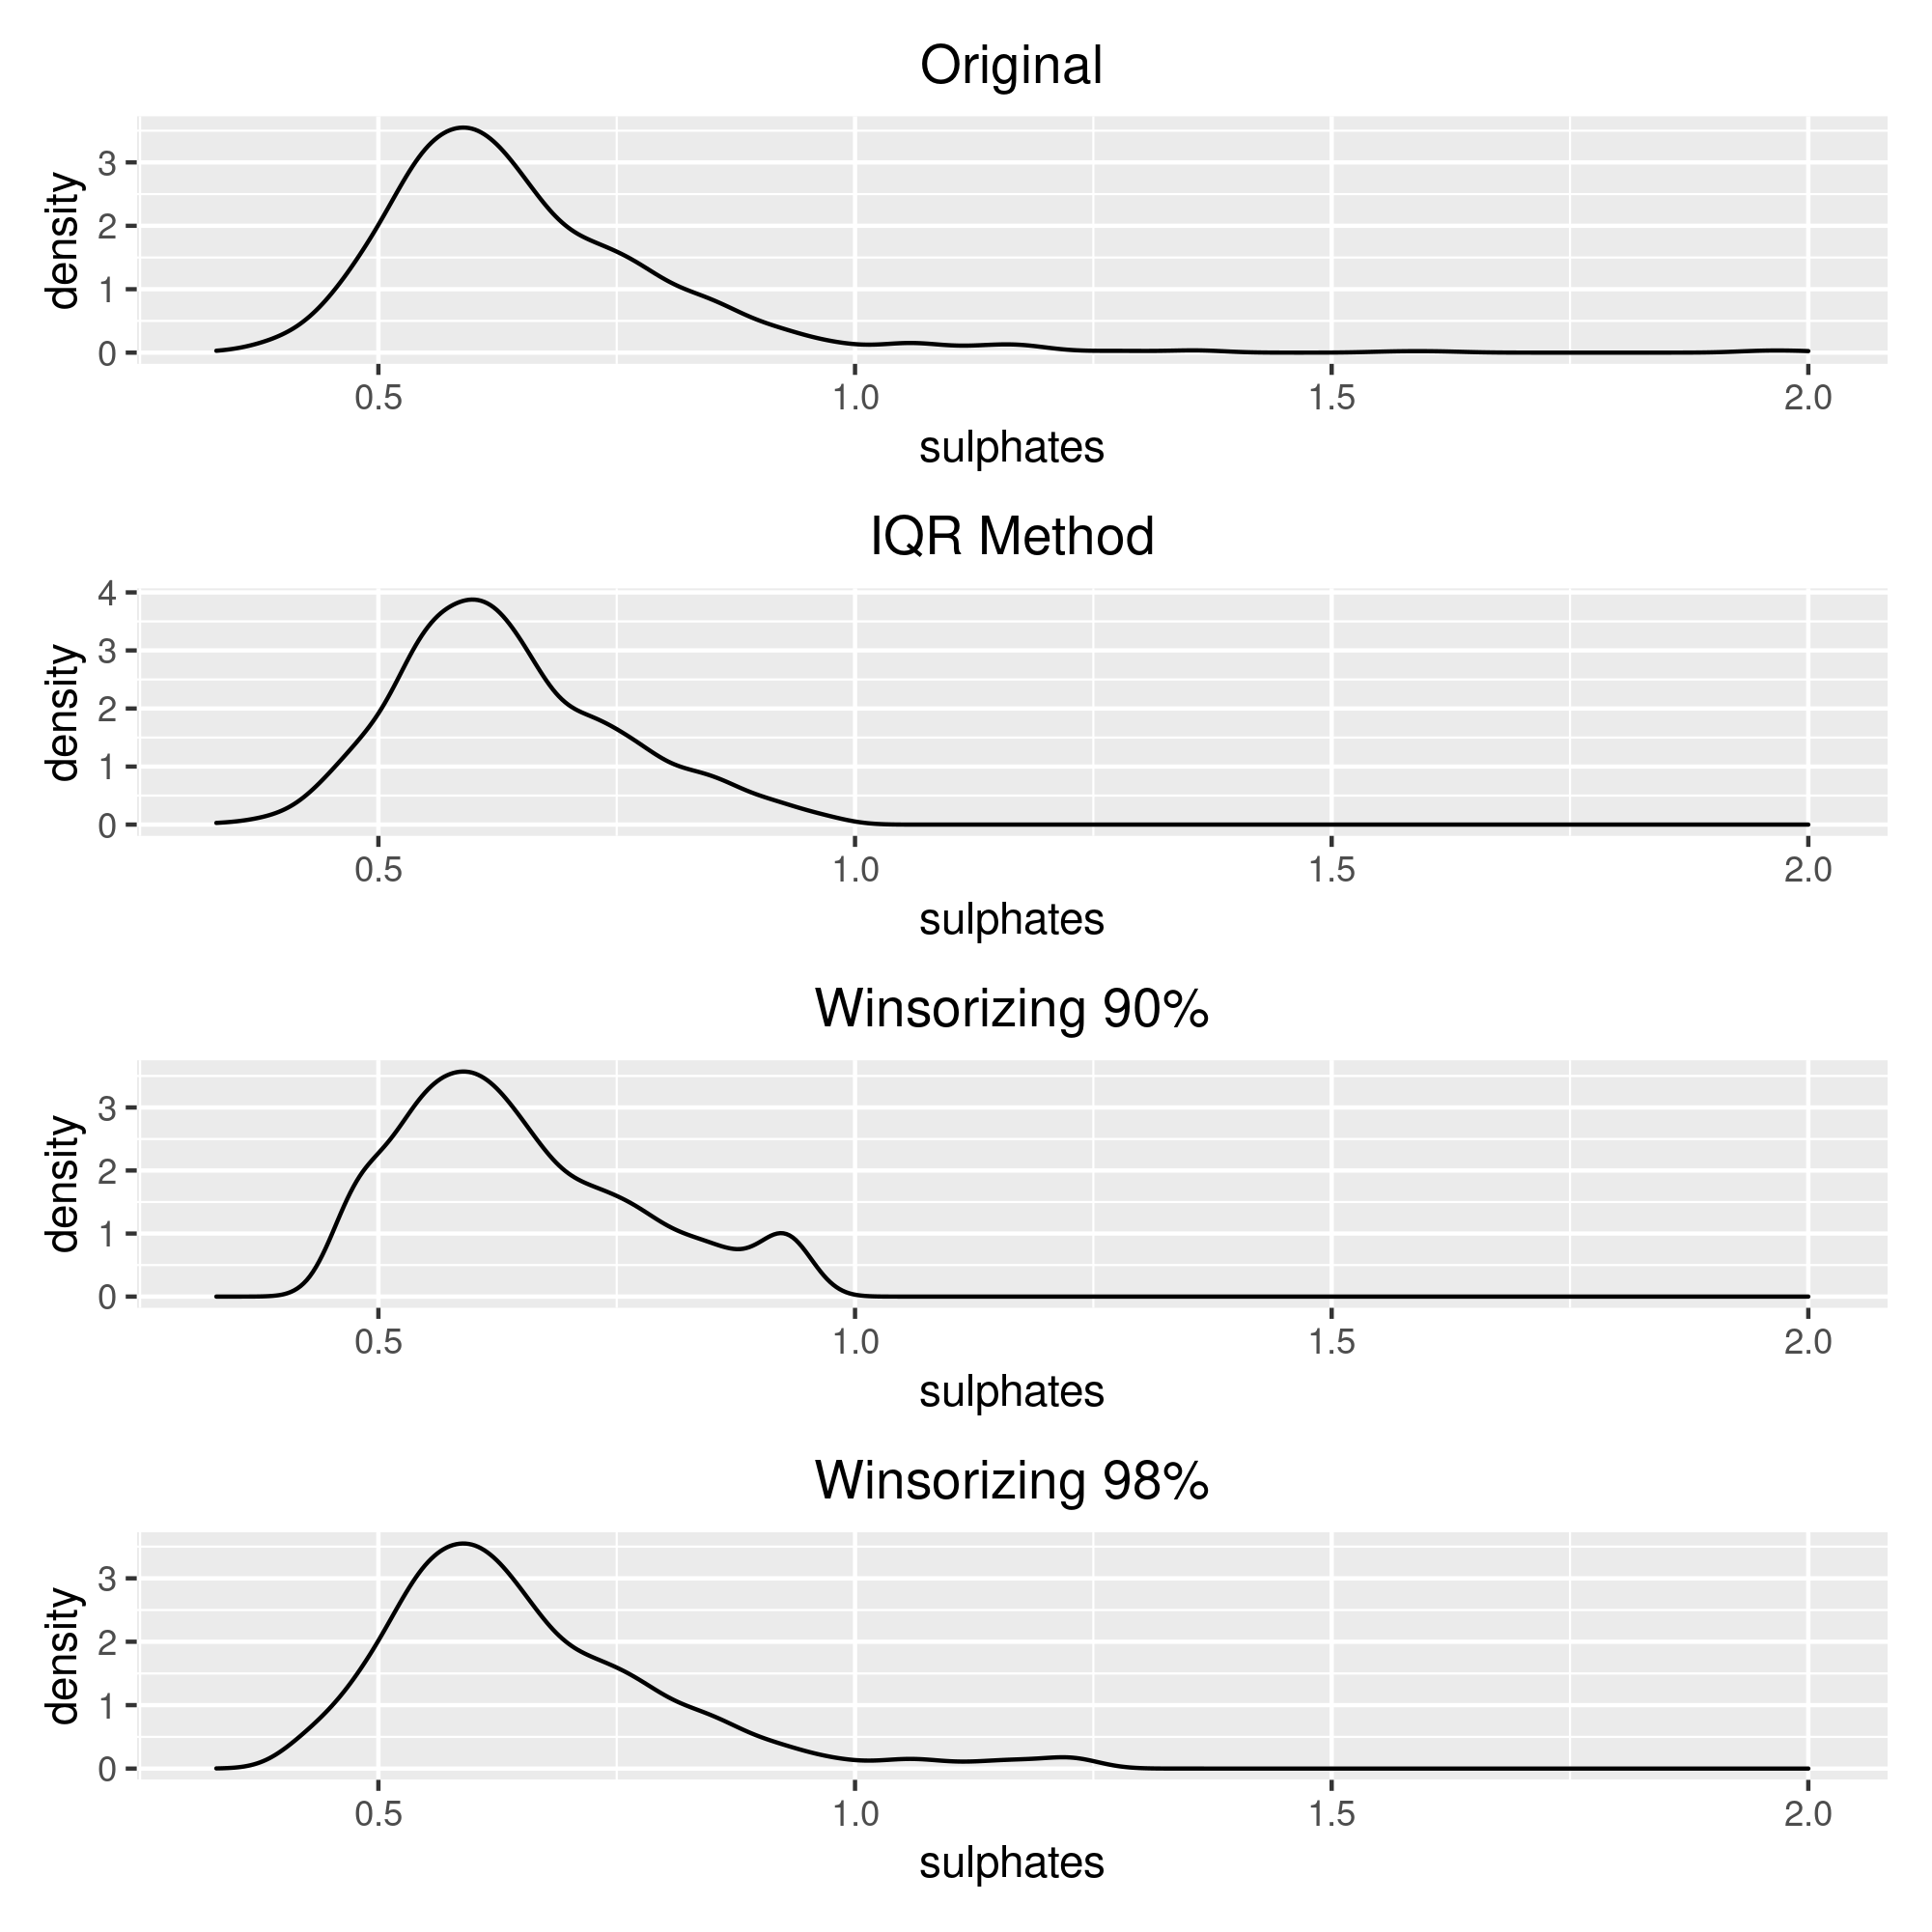
\includegraphics[width=0.45\textwidth]{images/outliers/sulphates_distribution.png}
    }\qquad
    \subfloat[]{%
        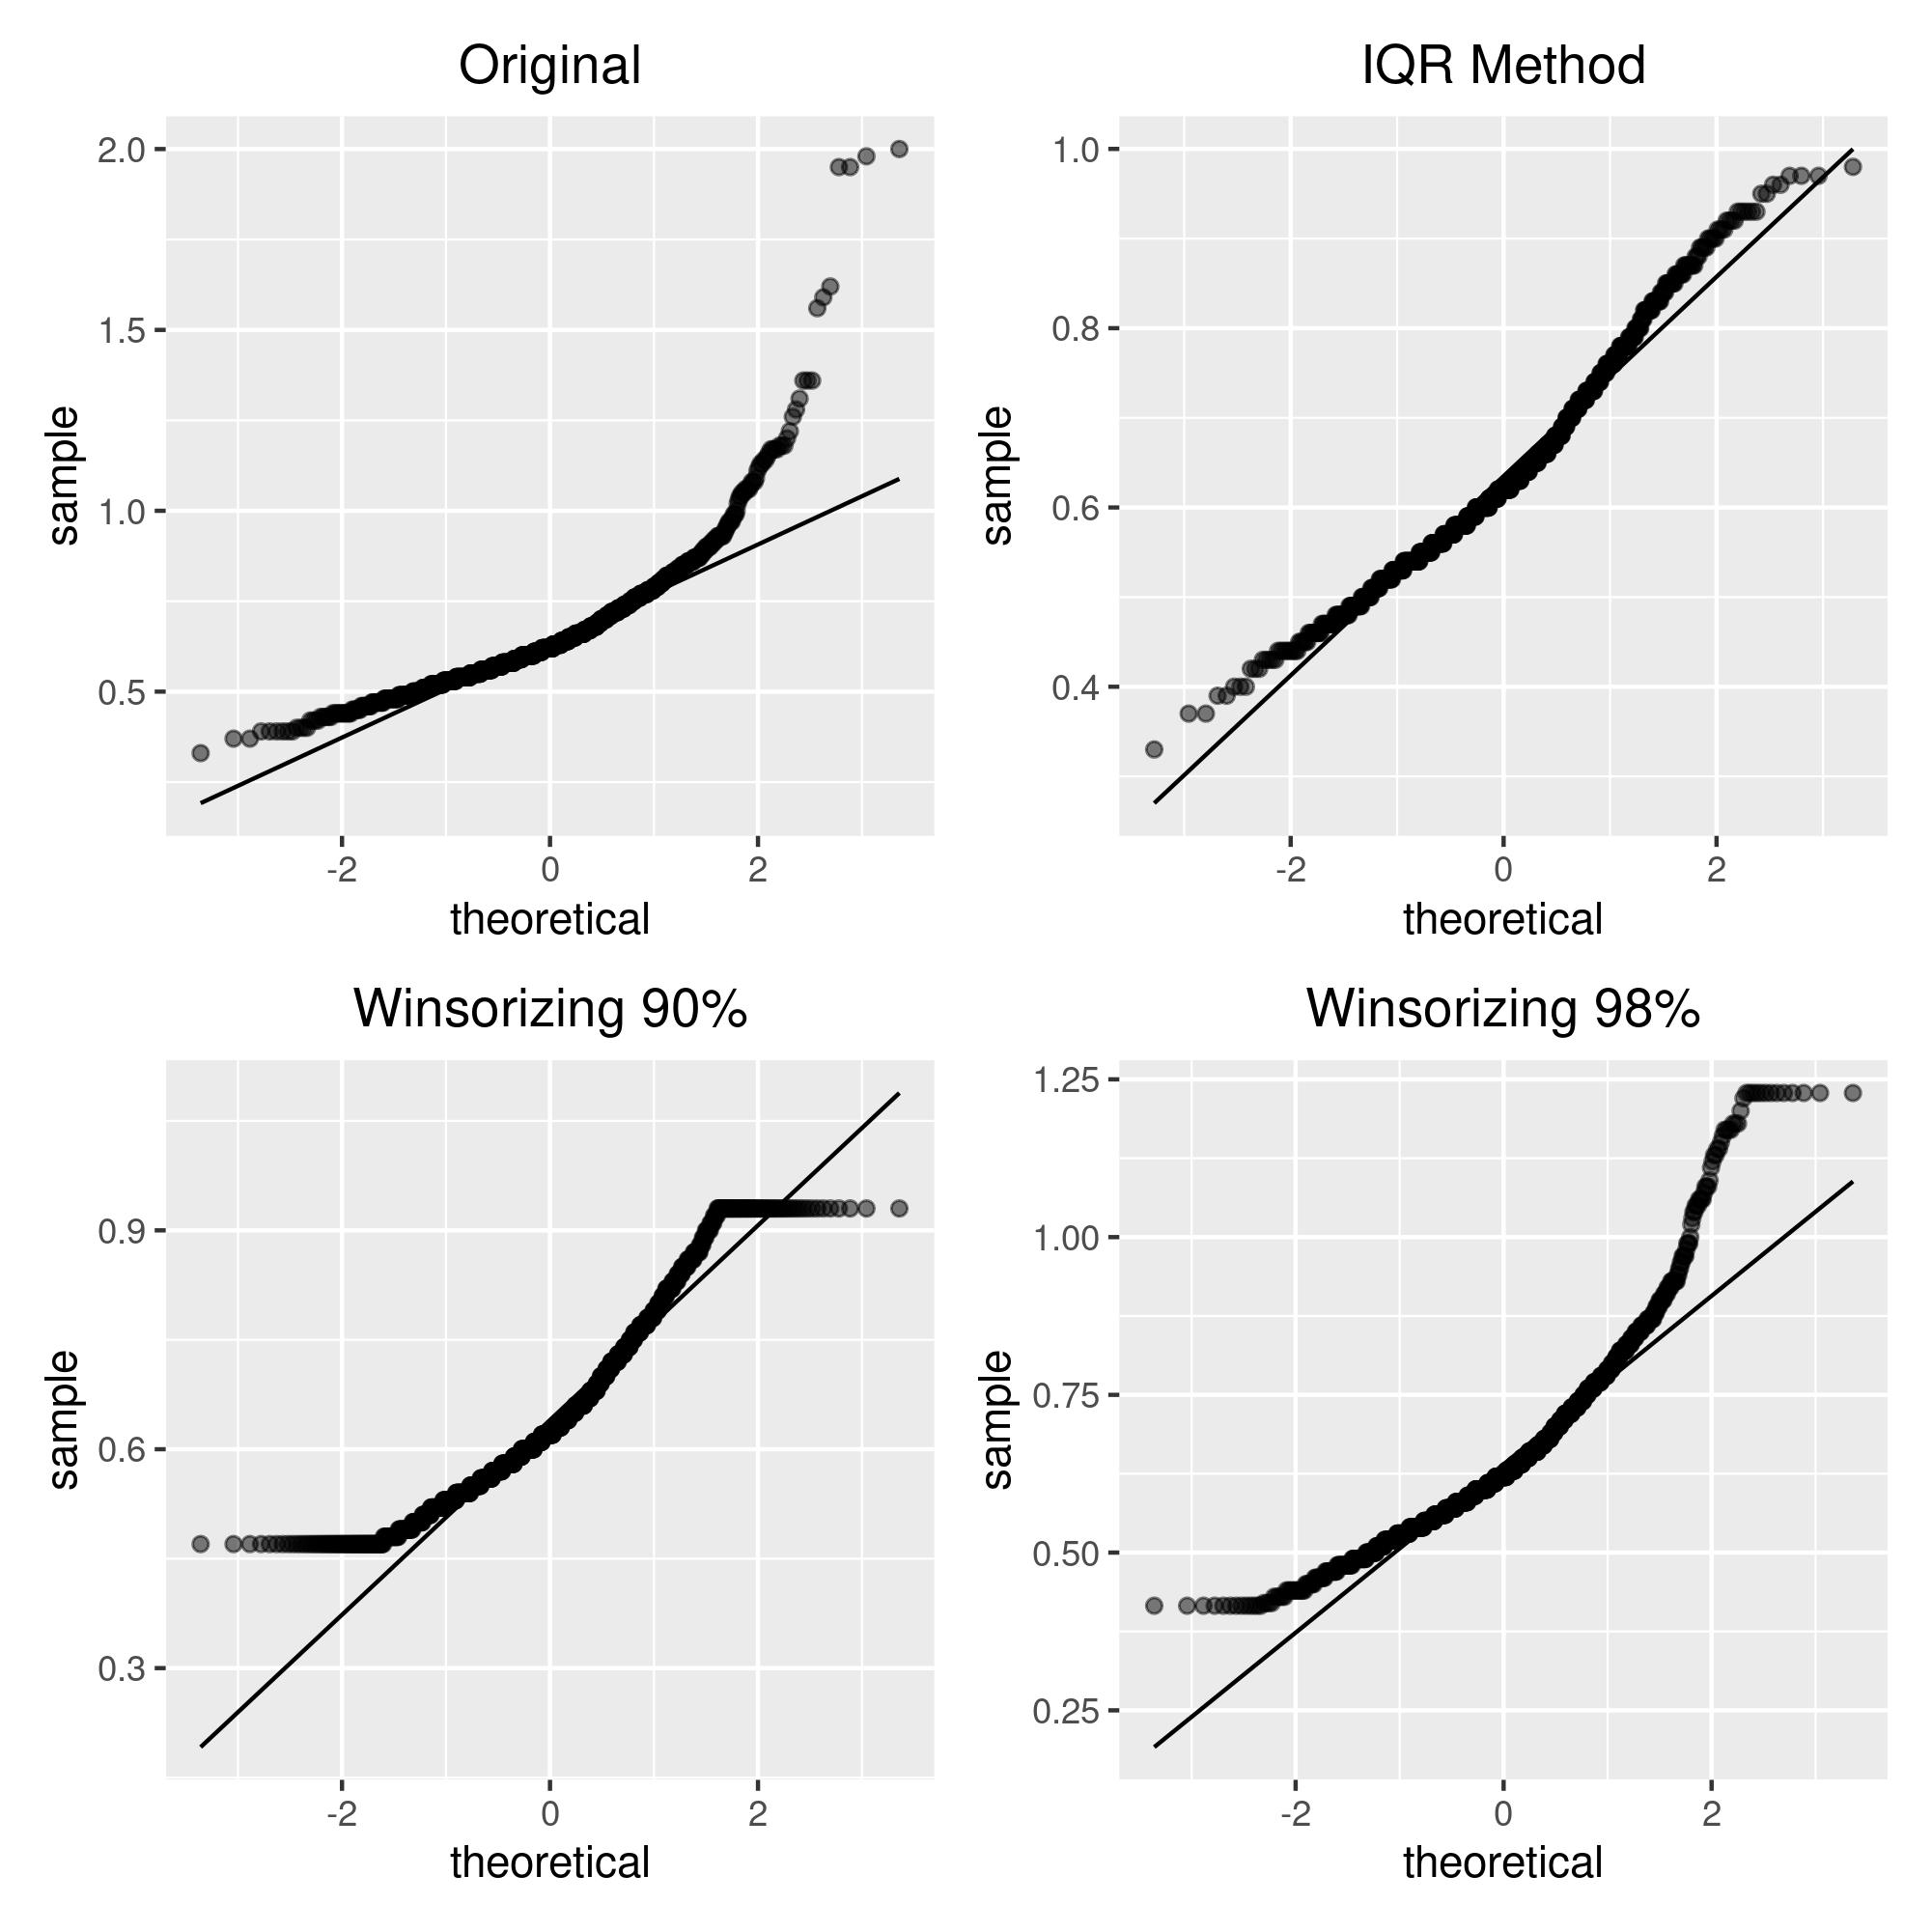
\includegraphics[width=0.45\textwidth]{images/outliers/sulphates_qqplot.png}
    }

    \label{fig:sulphates}
    \caption{Commento}
\end{figure}

\begin{figure}[H]
    \centering

    \subfloat[]{%
        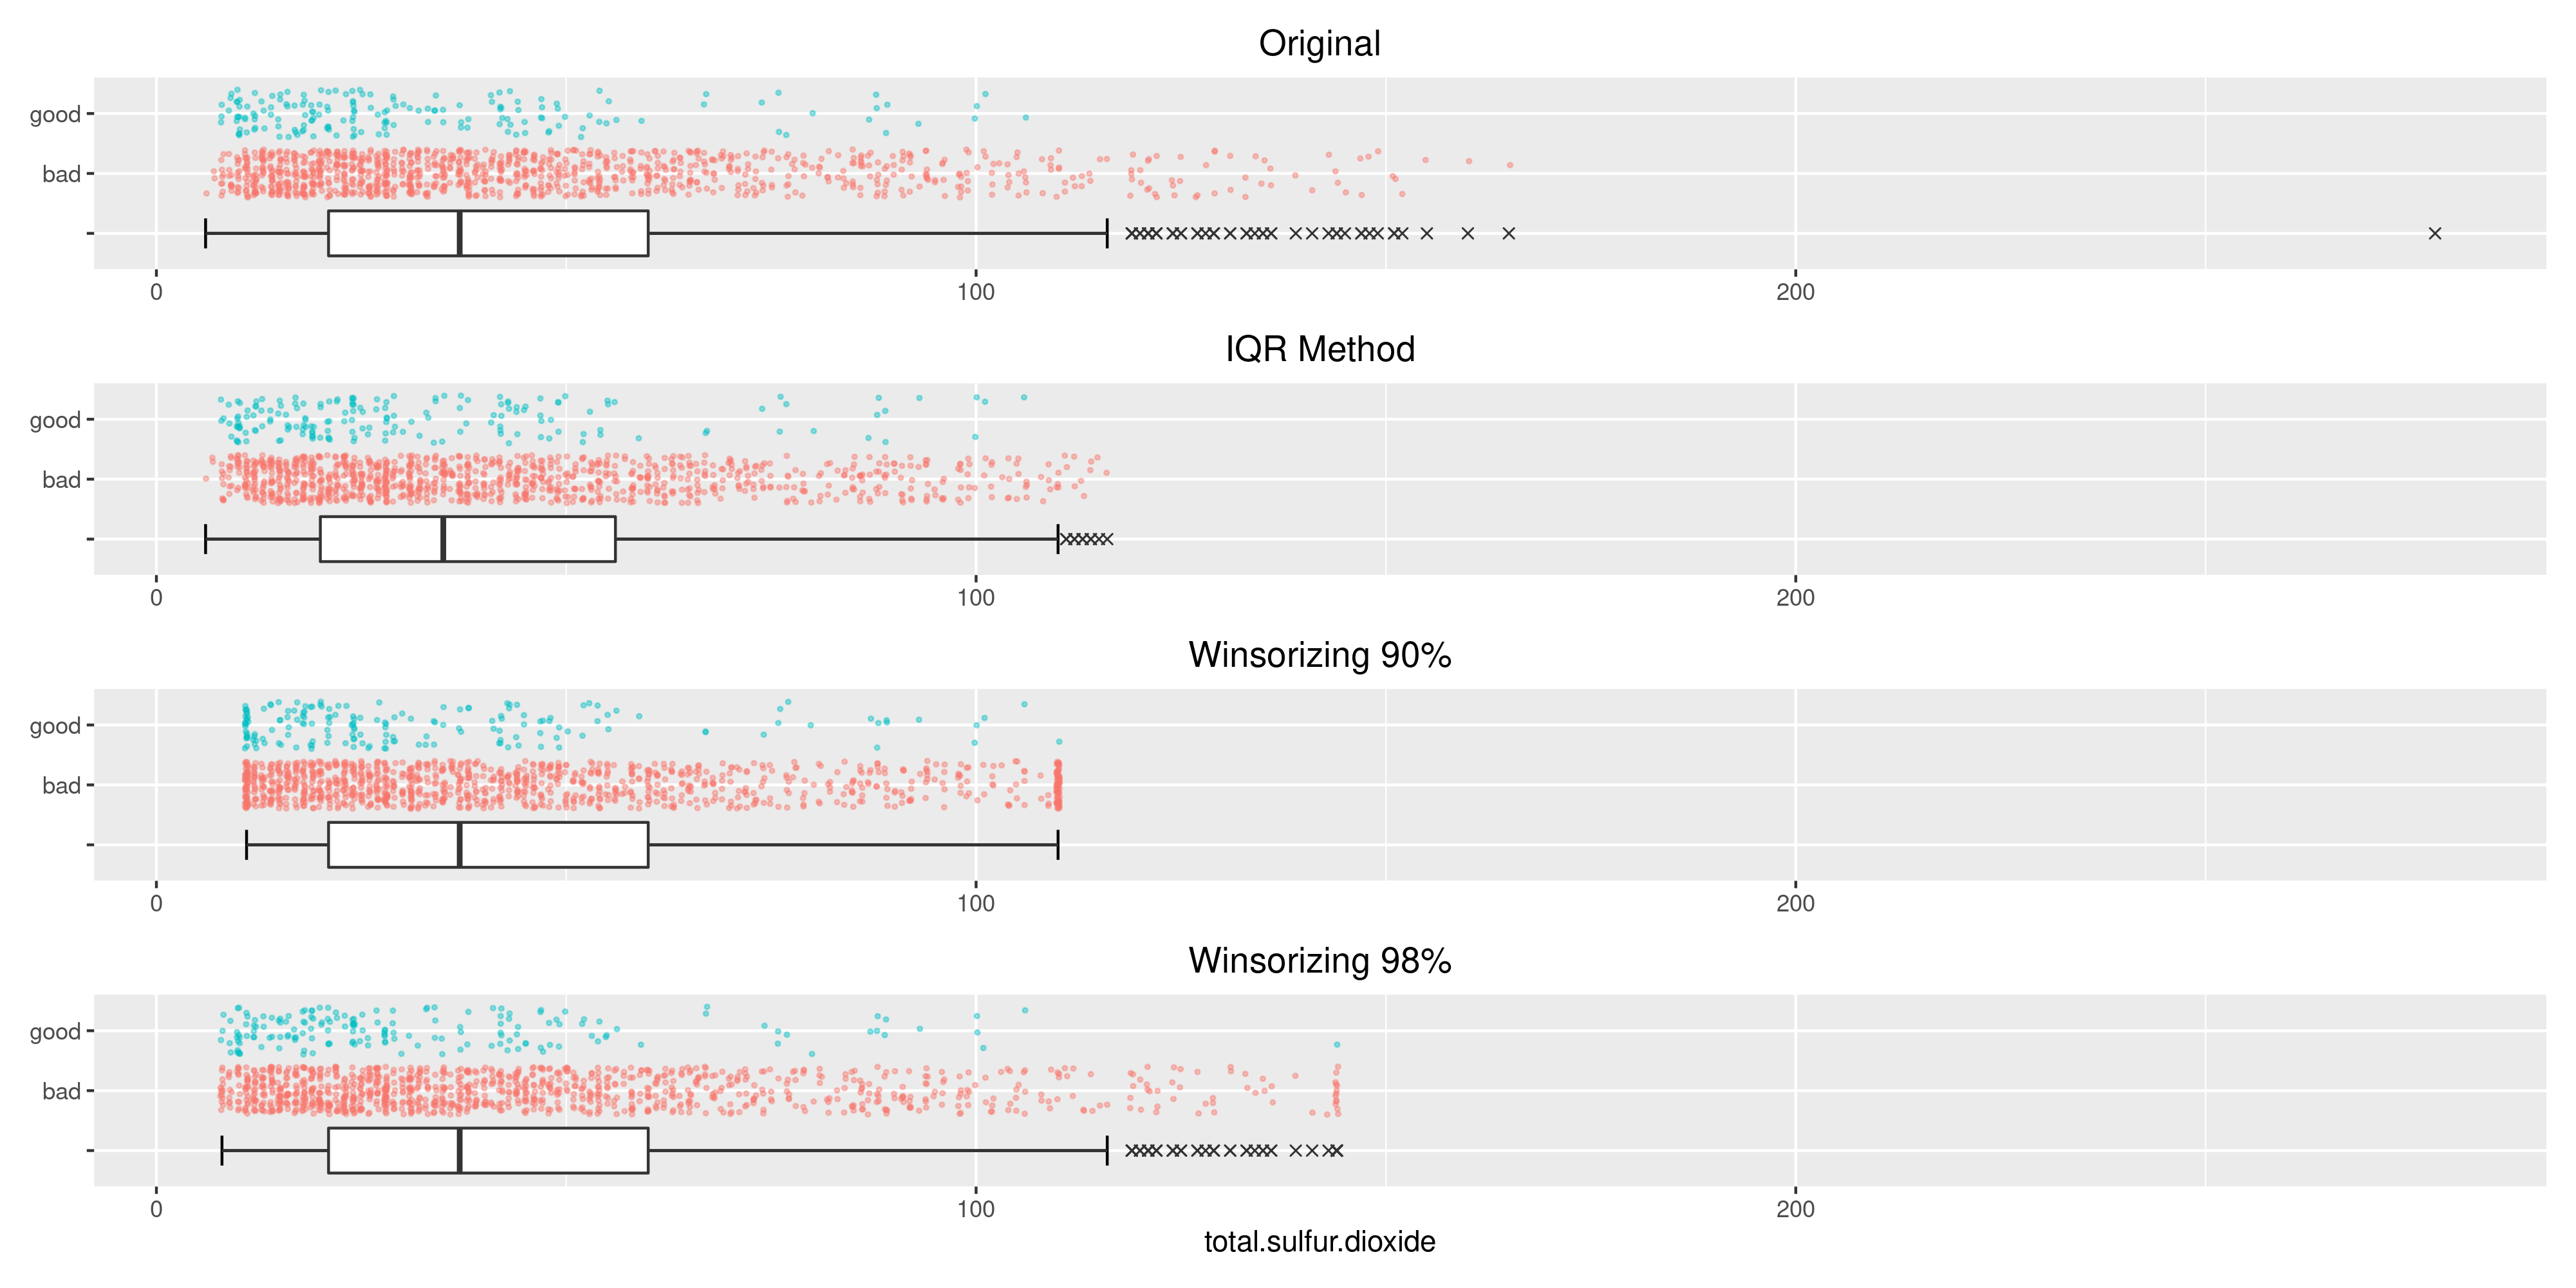
\includegraphics[width=0.99\textwidth]{images/outliers/total.sulfur.dioxide_boxplot.png}
    }

    \subfloat[]{%
        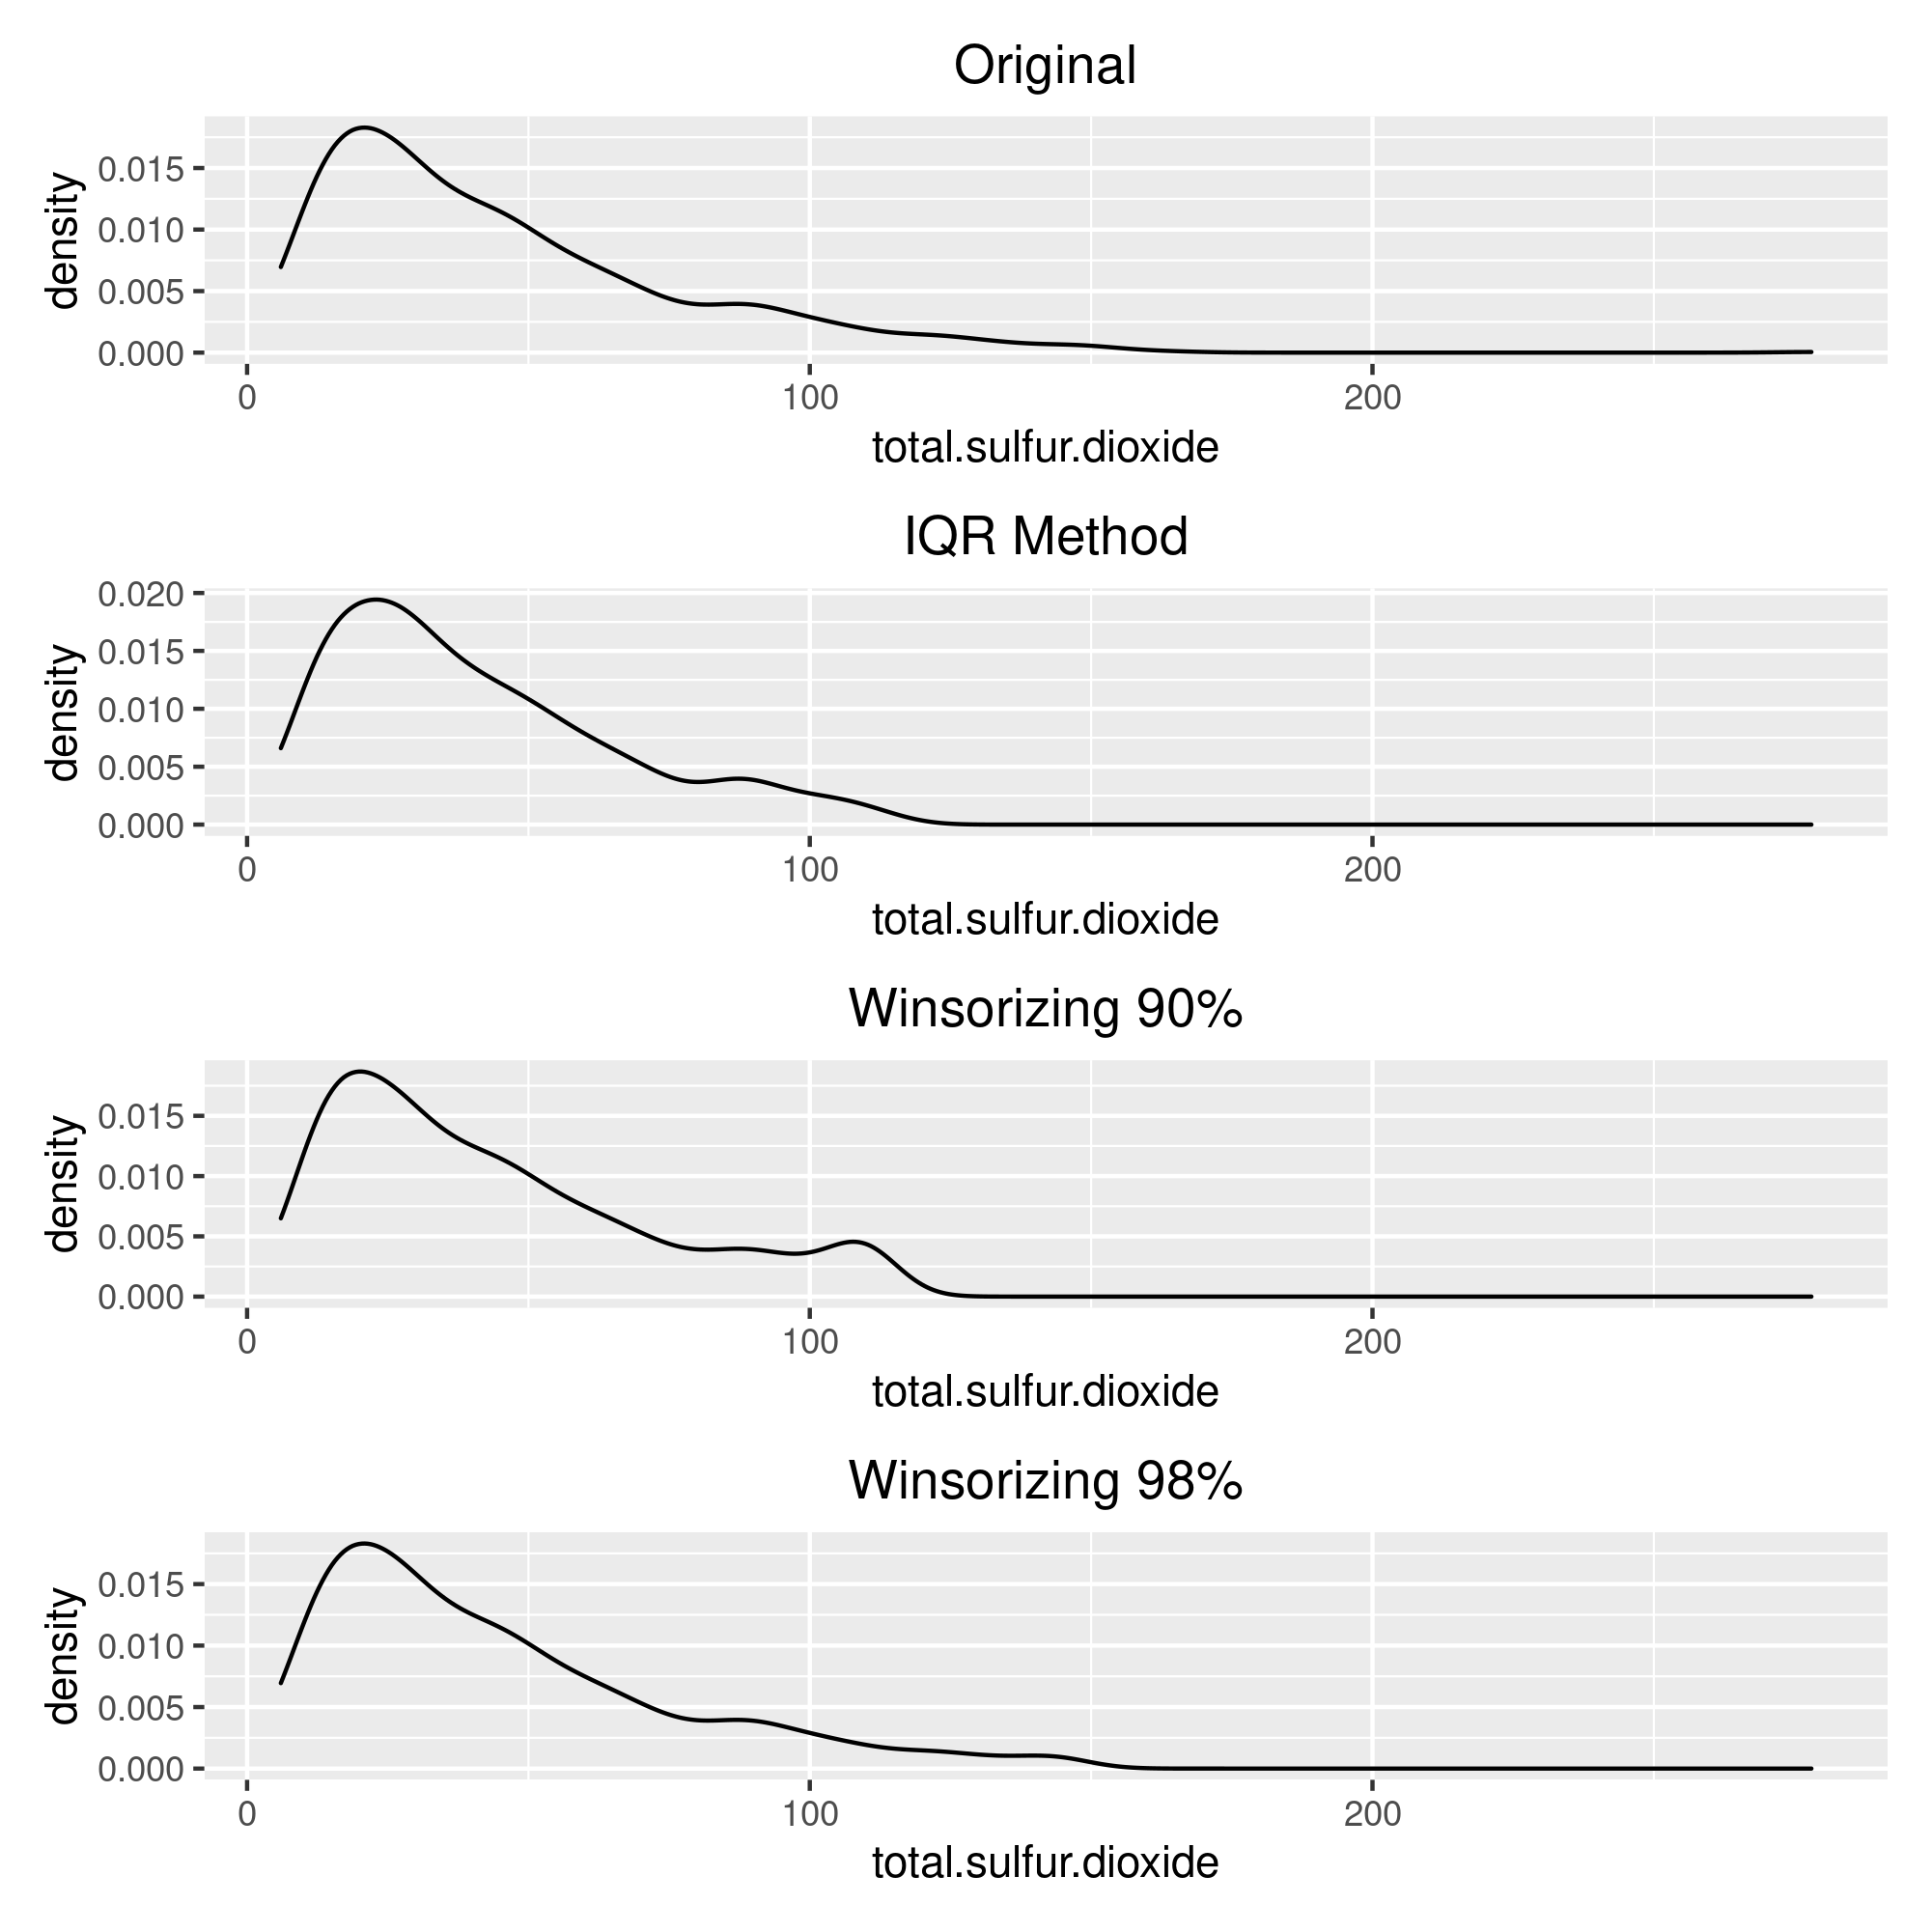
\includegraphics[width=0.45\textwidth]{images/outliers/total.sulfur.dioxide_distribution.png}
    }\qquad
    \subfloat[]{%
        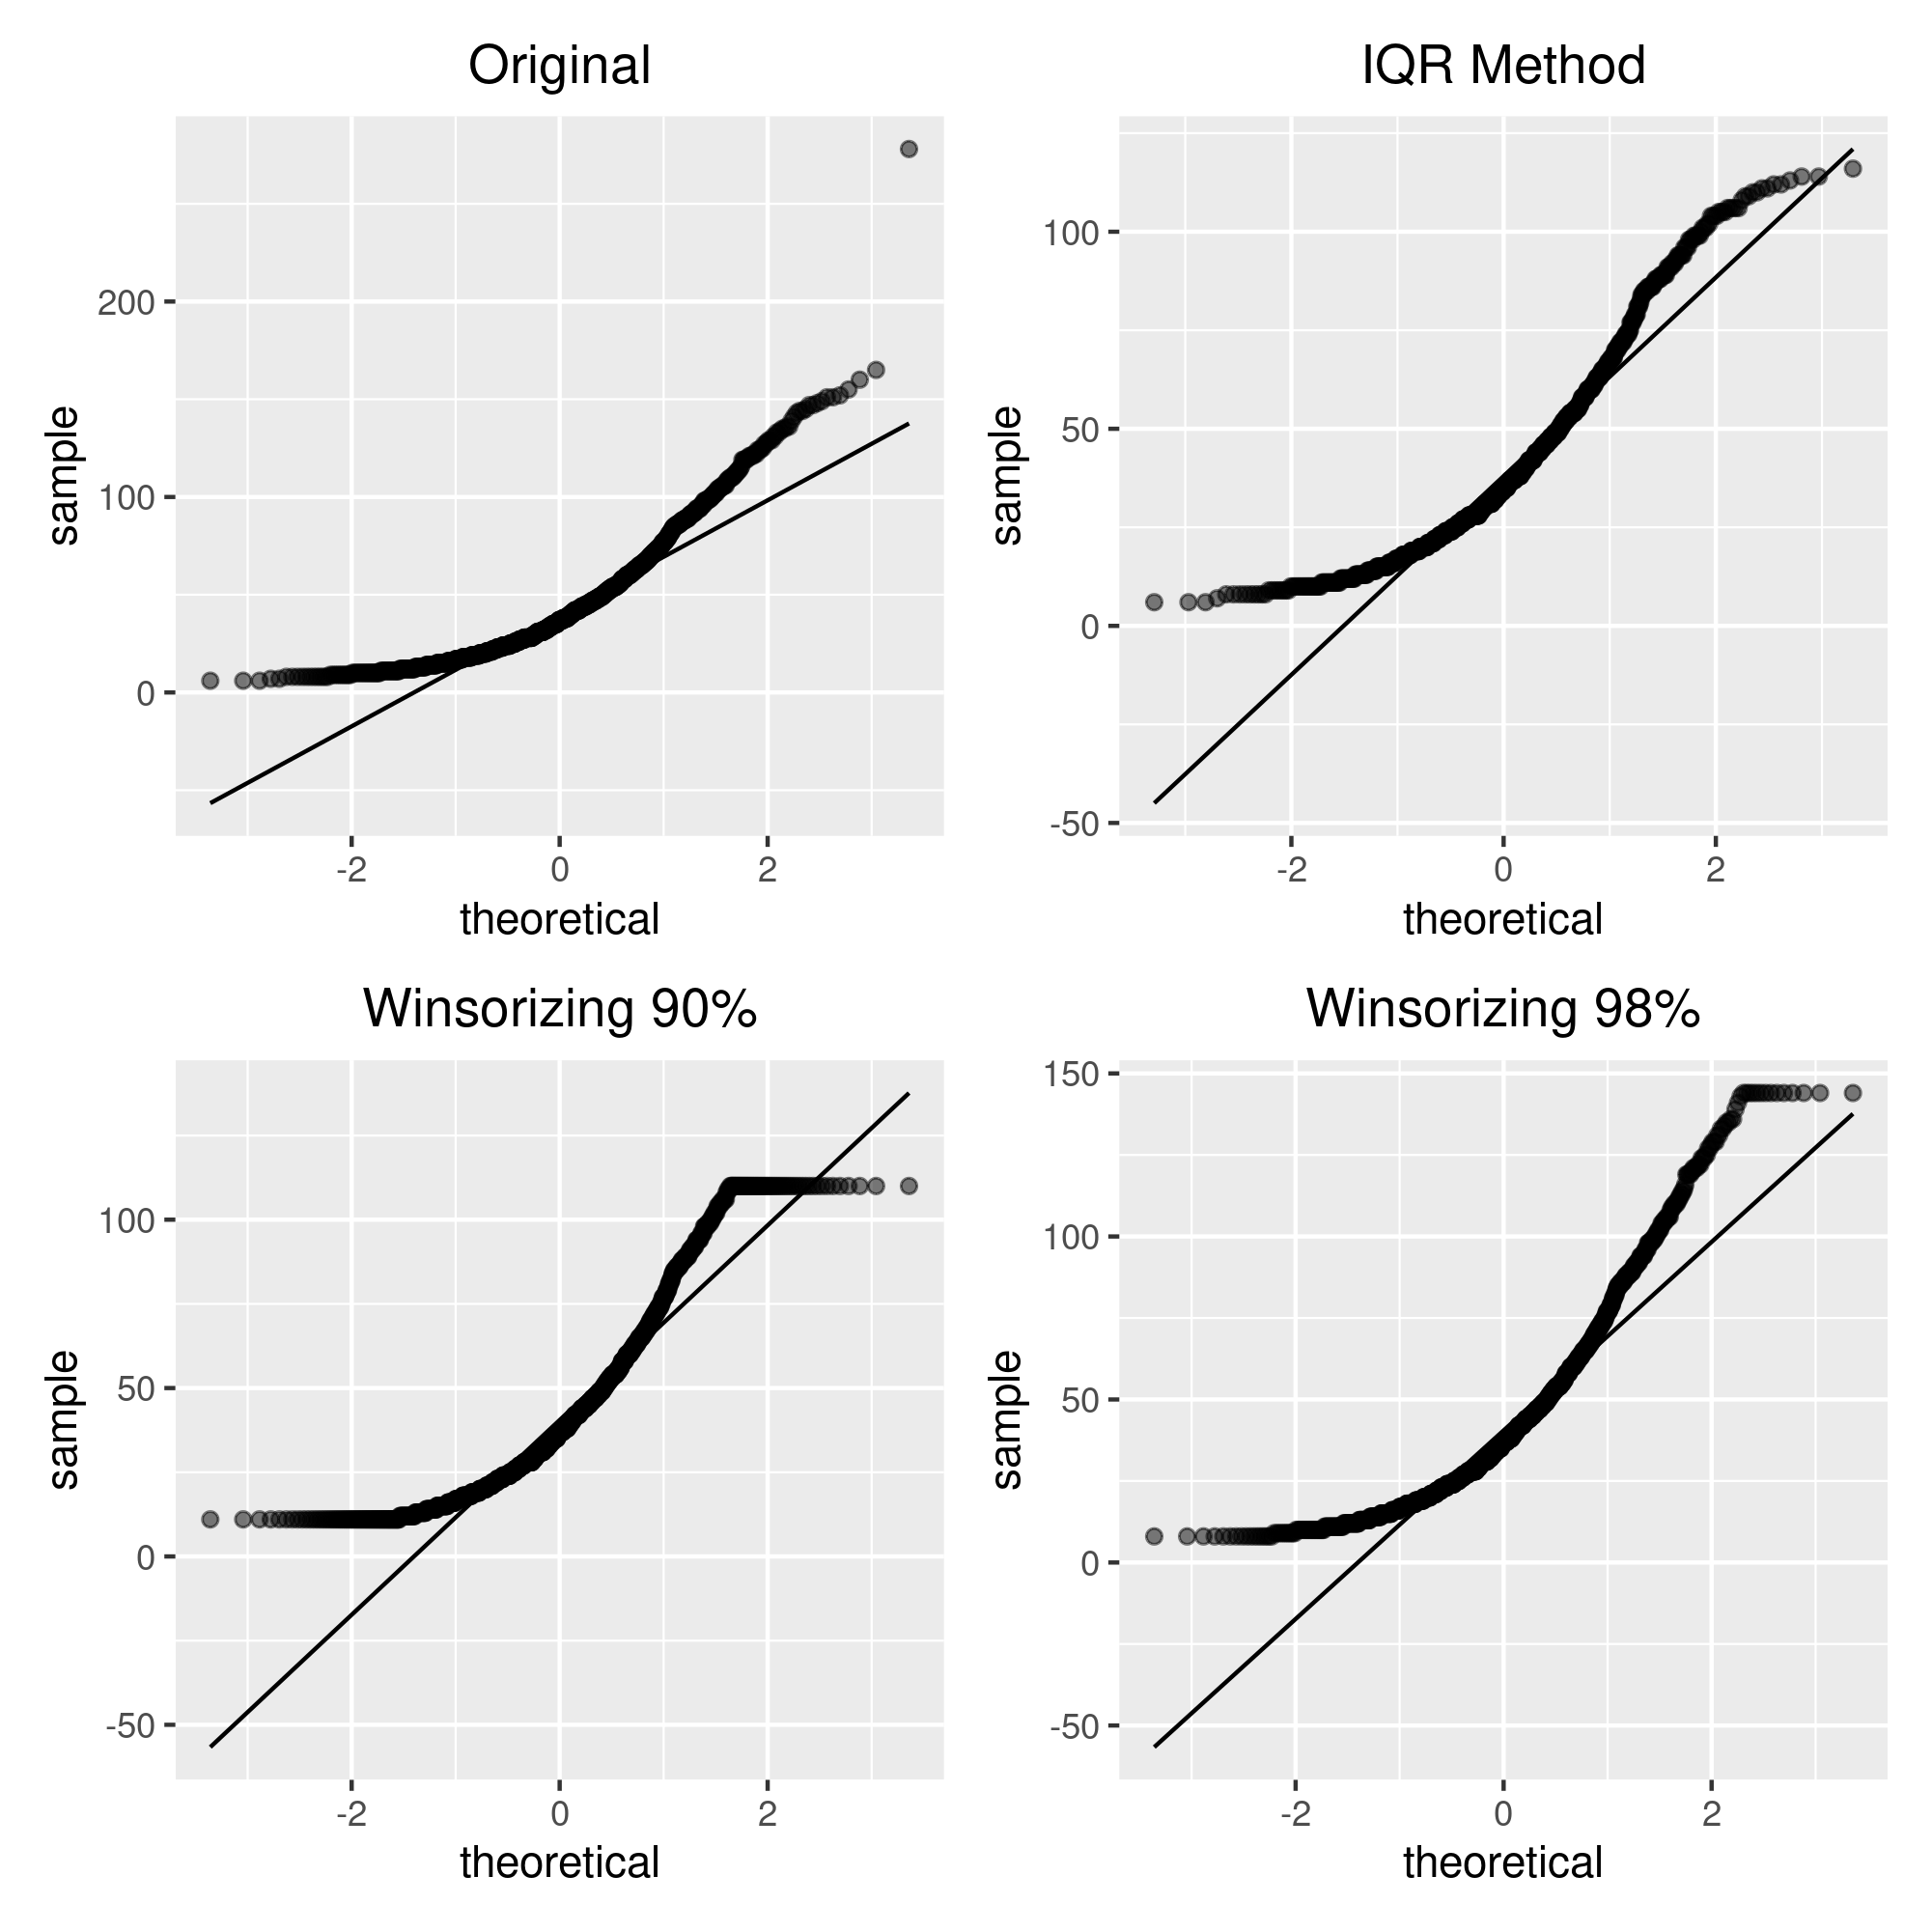
\includegraphics[width=0.45\textwidth]{images/outliers/total.sulfur.dioxide_qqplot.png}
    }

    \label{fig:total.sulfur.dioxide}
    \caption{Commento}
\end{figure}

\begin{figure}[H]
    \centering

    \subfloat[]{%
        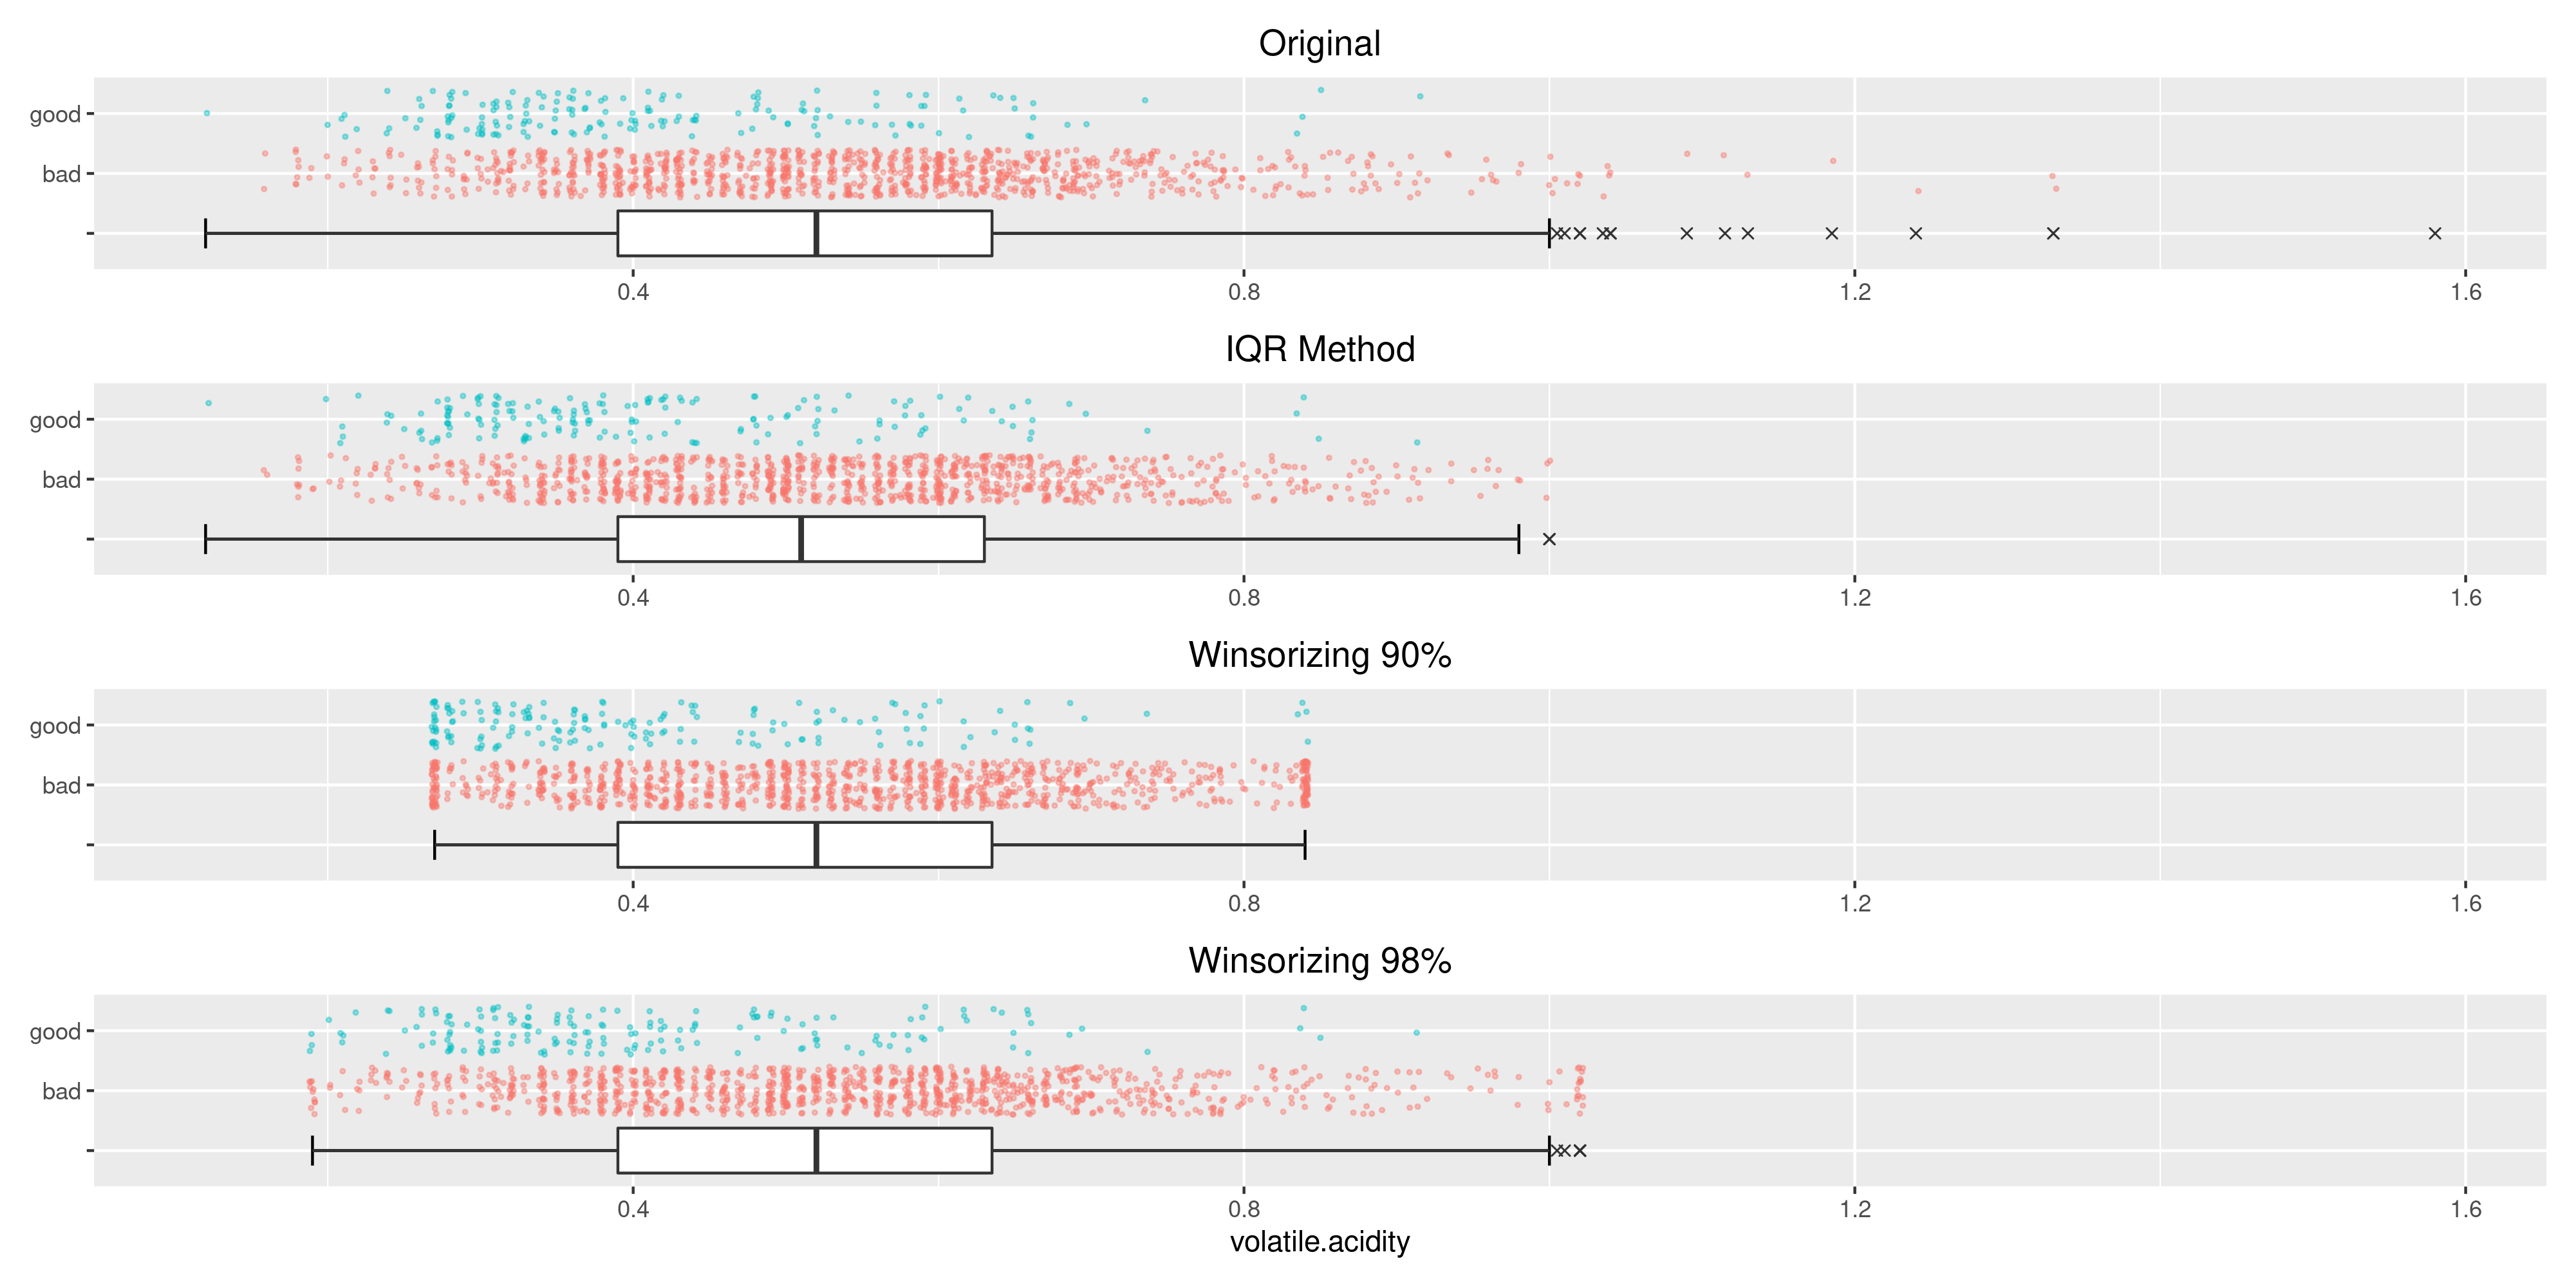
\includegraphics[width=0.99\textwidth]{images/outliers/volatile.acidity_boxplot.png}
    }

    \subfloat[]{%
        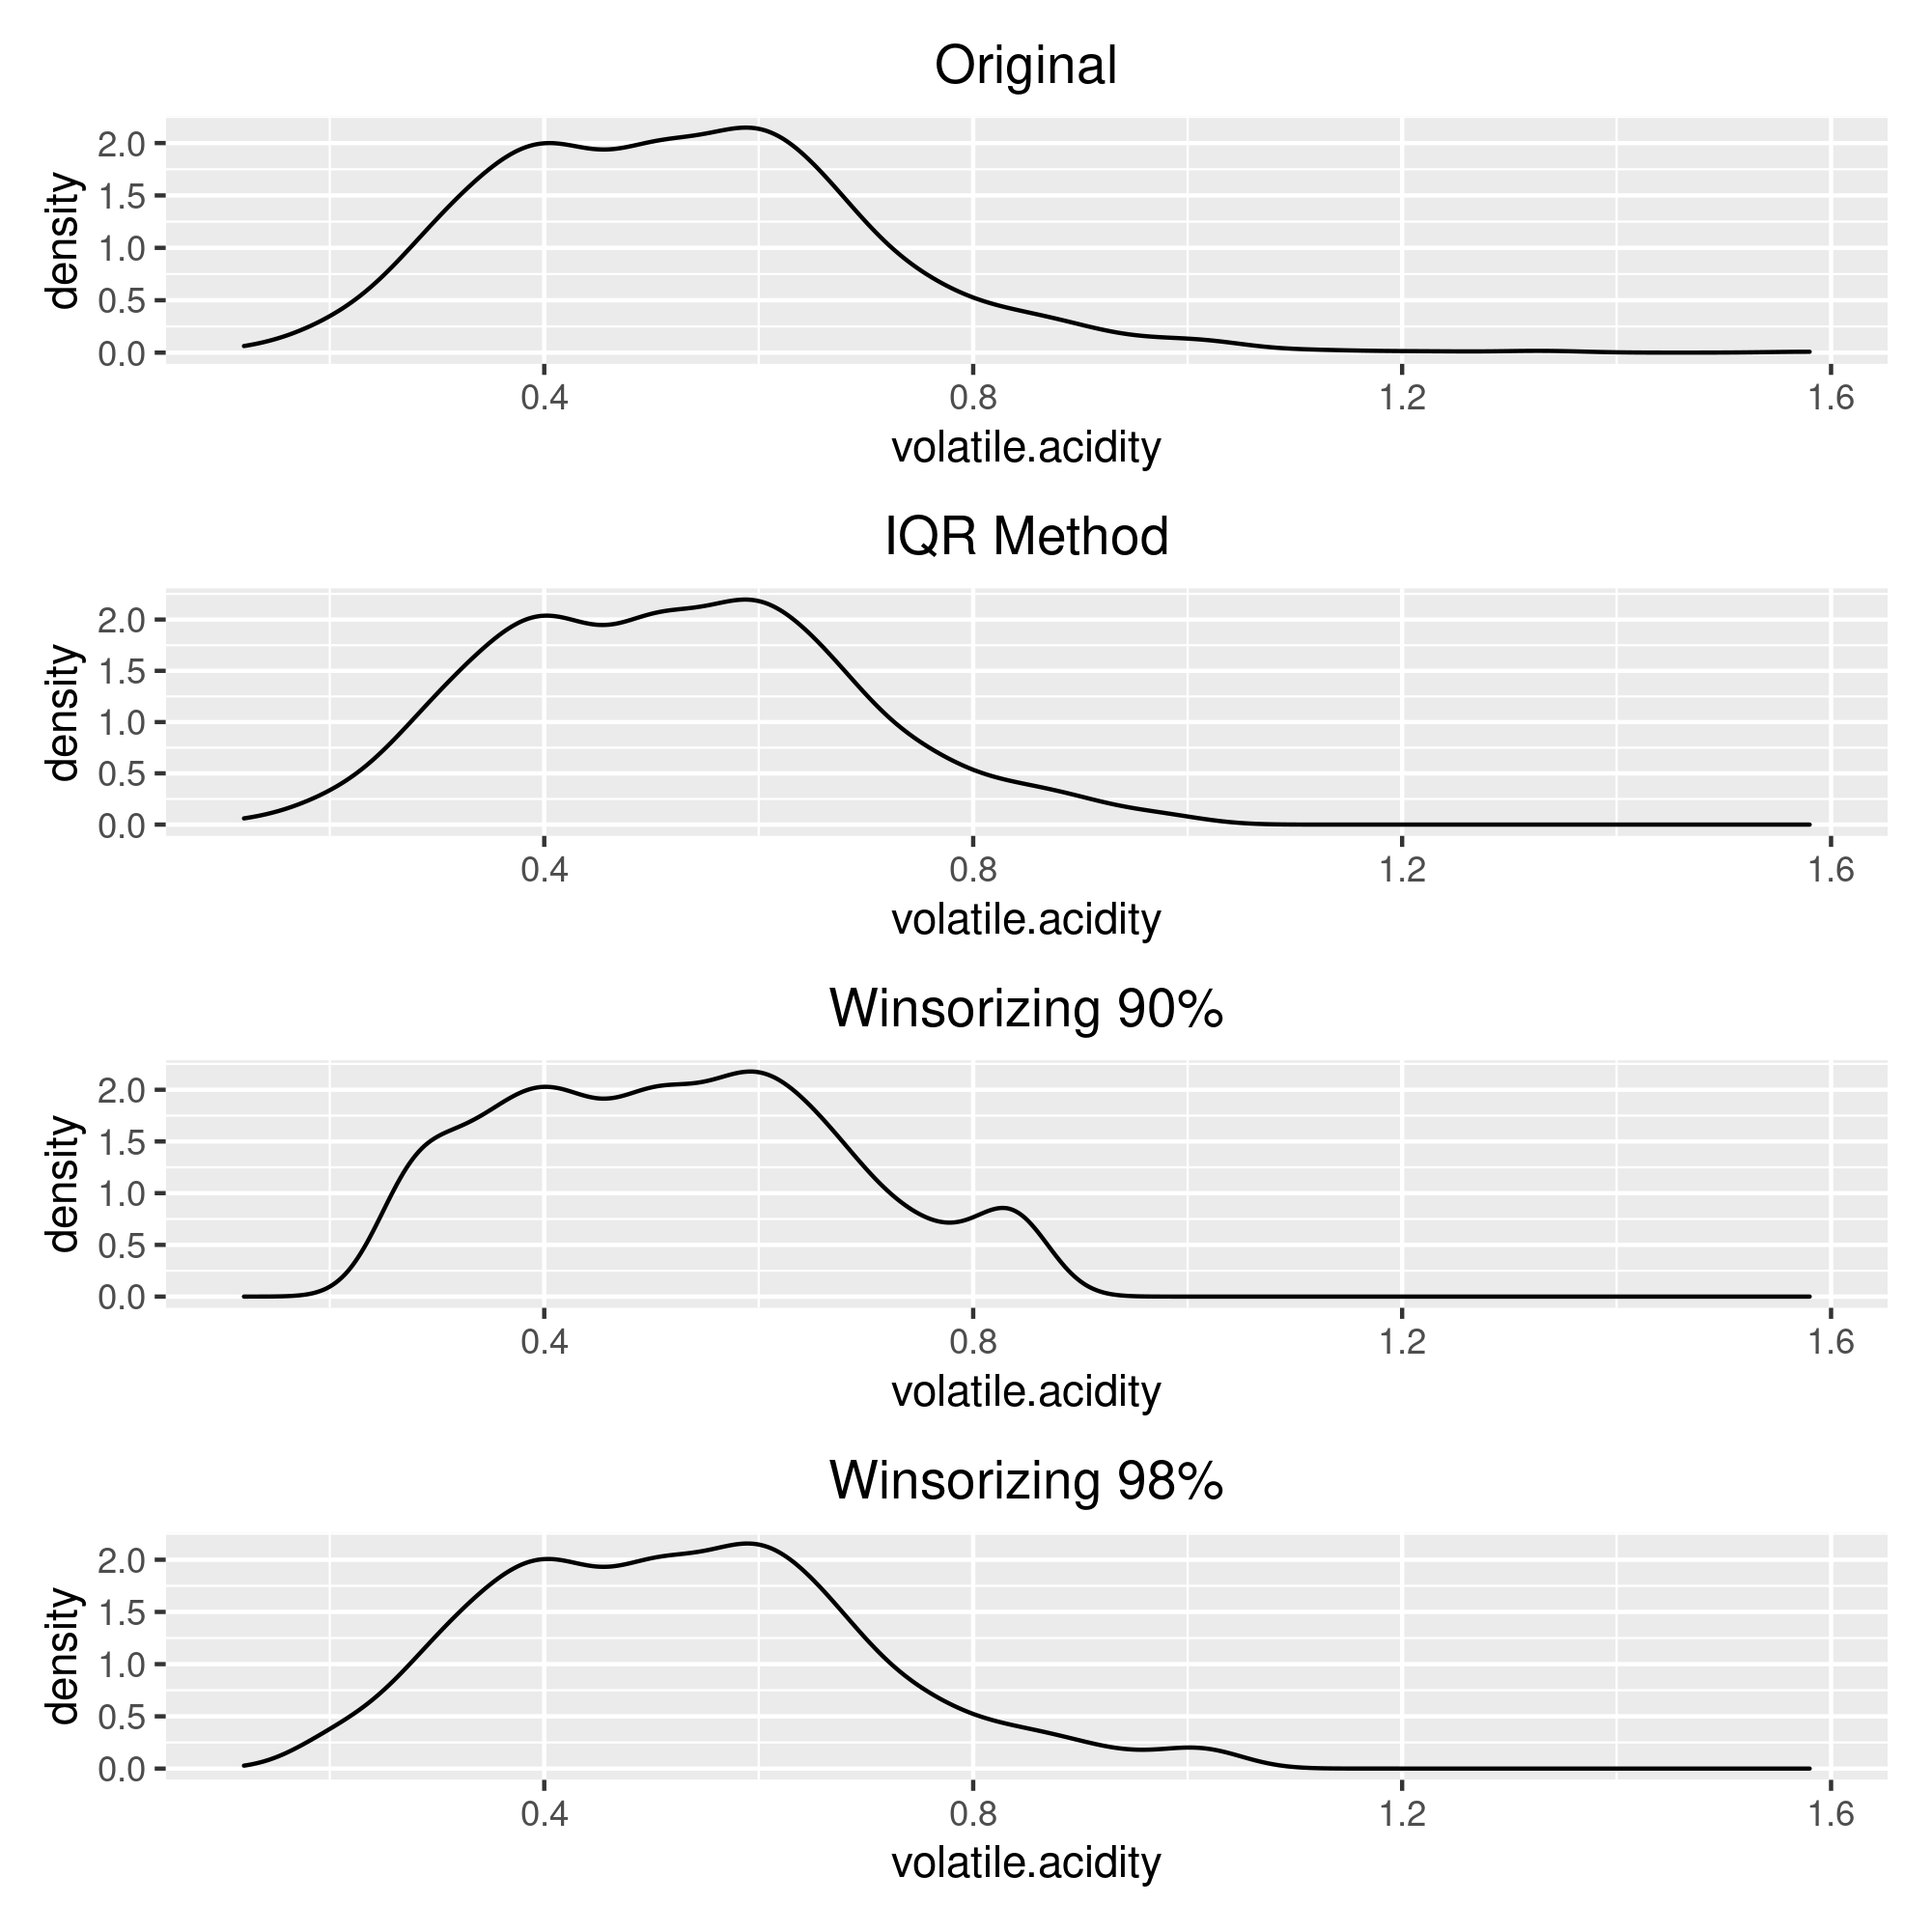
\includegraphics[width=0.45\textwidth]{images/outliers/volatile.acidity_distribution.png}
    }\qquad
    \subfloat[]{%
        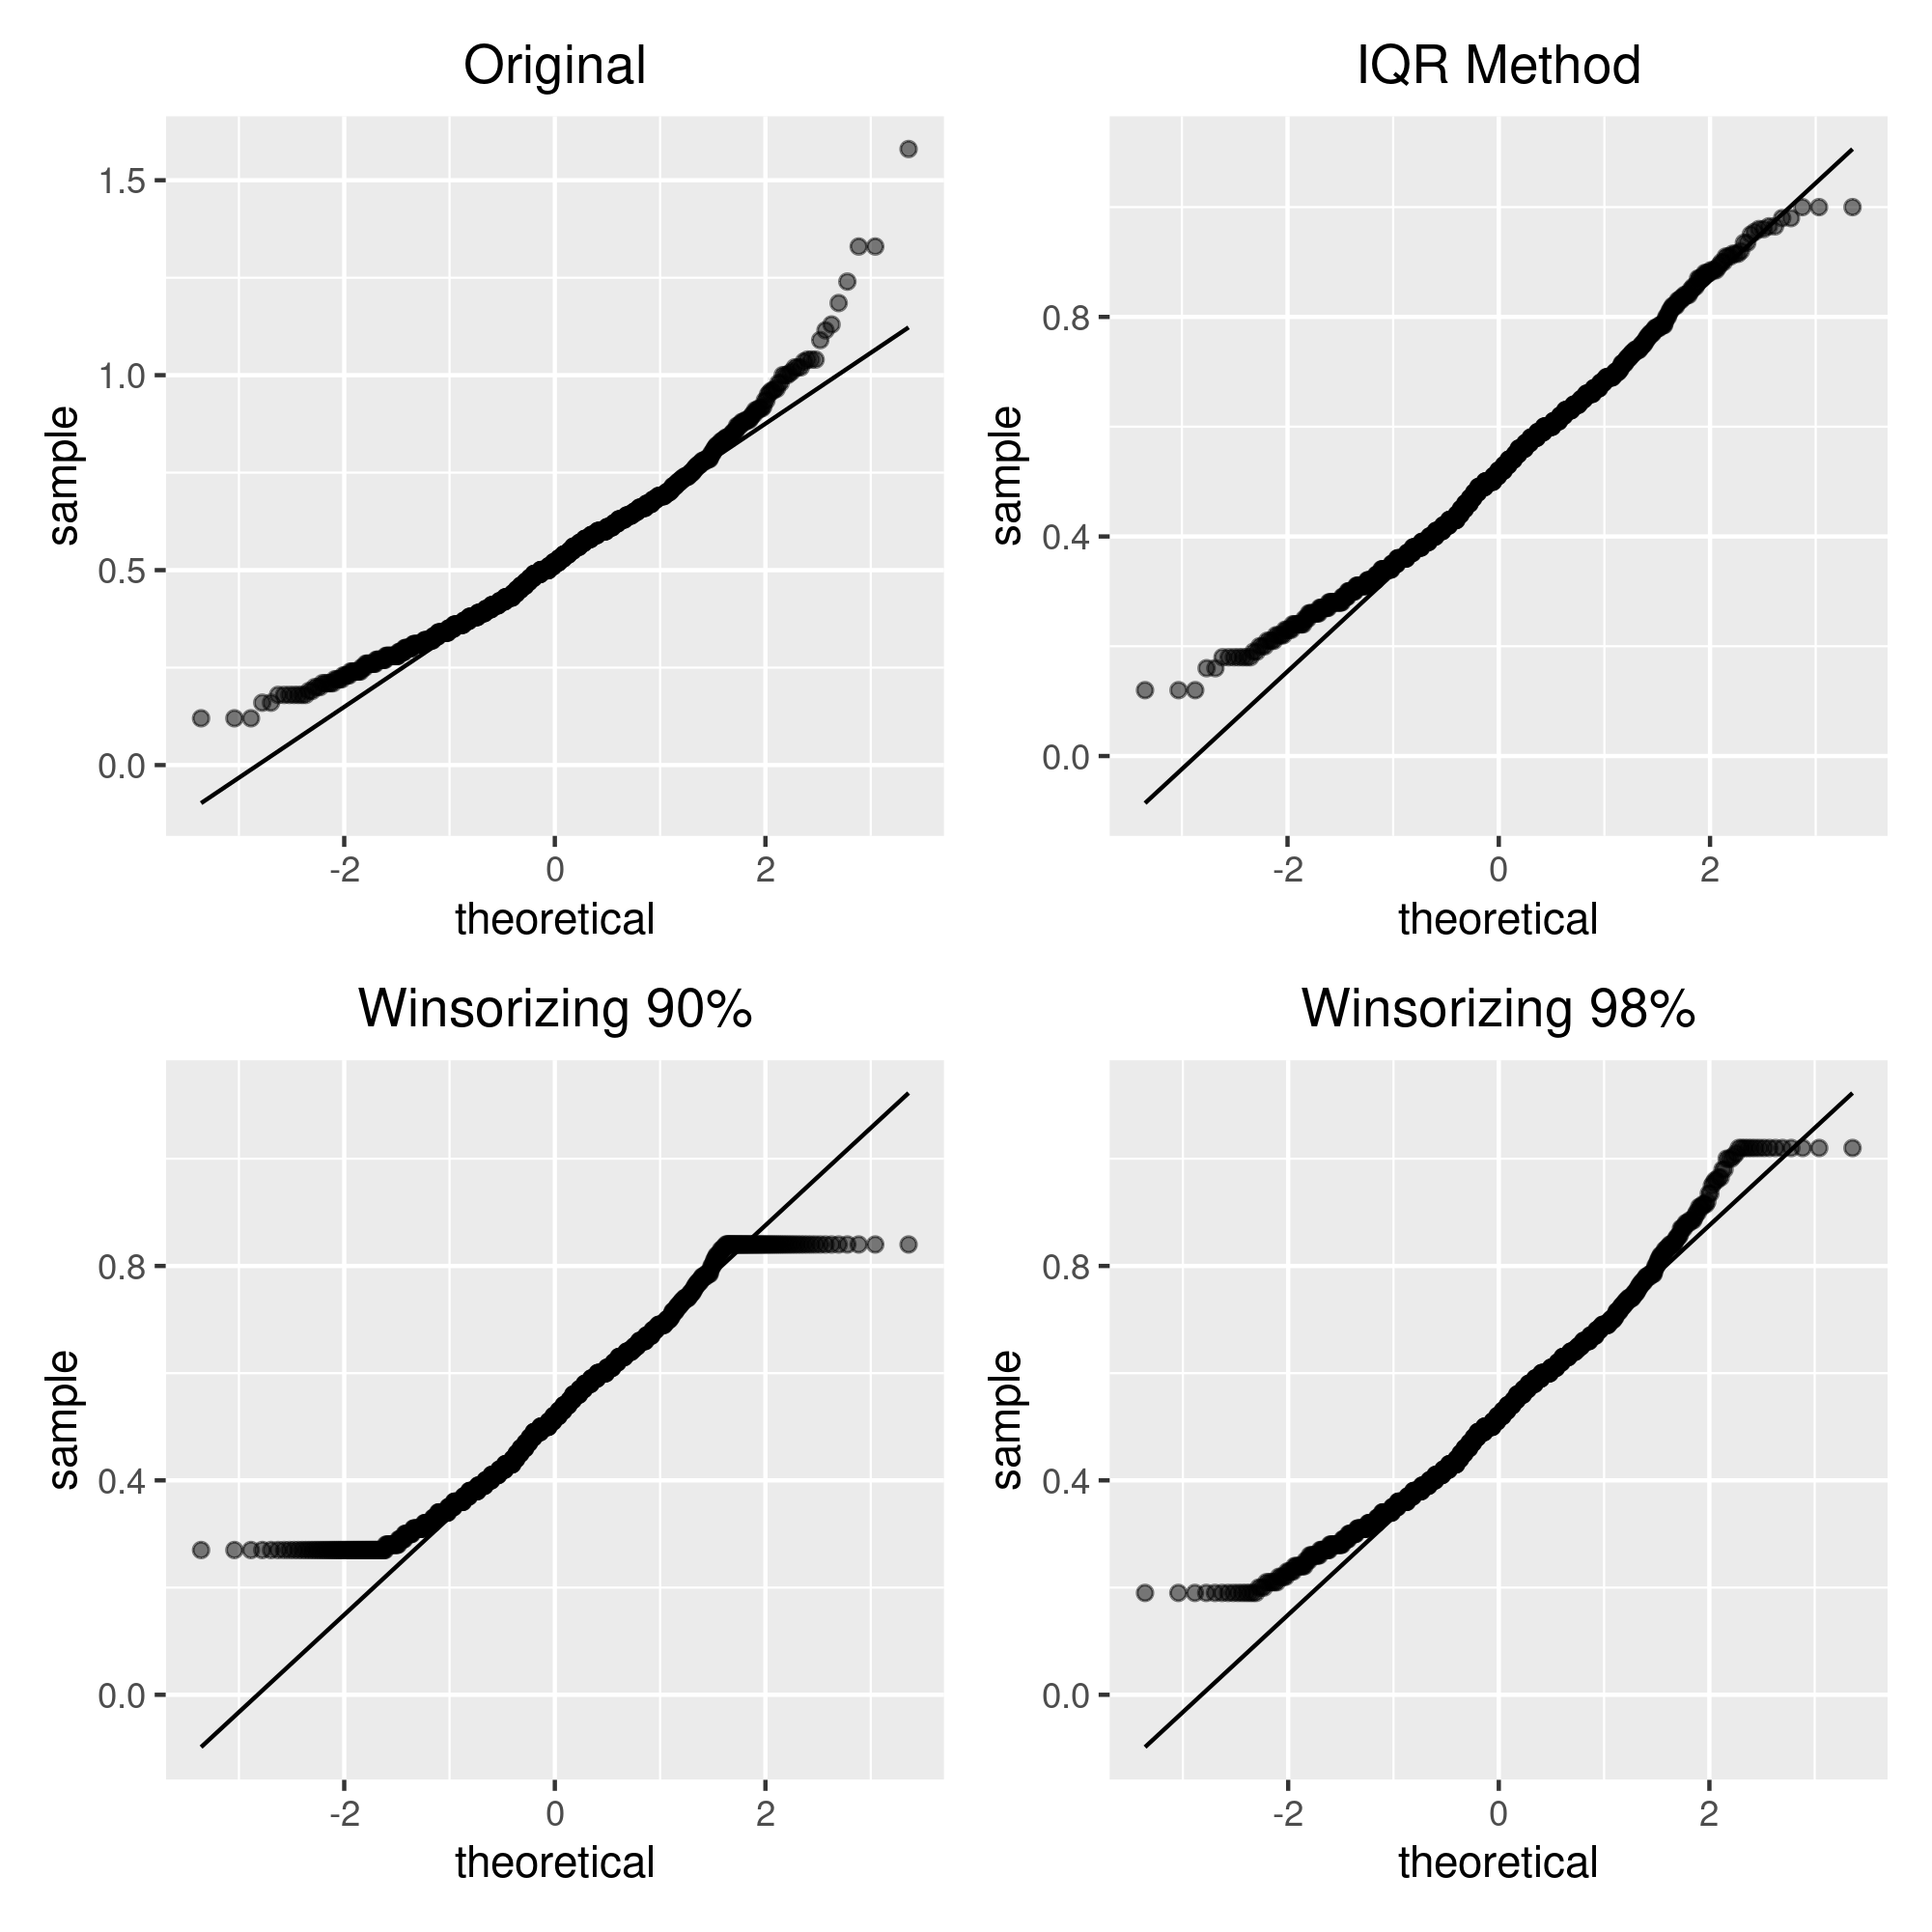
\includegraphics[width=0.45\textwidth]{images/outliers/volatile.acidity_qqplot.png}
    }

    \label{fig:volatile.acidity}
    \caption{Commento}
\end{figure}


\section{Distribuzioni delle variabili}
In questo capitolo si è analizzata la distribuzione per ogni singola variabile.\\
Per ogni grafico sull'asse delle ordinate si trova il range di valori assunti dalle istanze nel dataset mentre sull'asse delle ascisse si trova il numero di istanze che assume il determinato valore rispetto alla singola variabile analizzata.\\
Questa è un analisi univariata ovvero viene considerata una singola variabile alla volta, osserveremo solo una variabile per ogni grafico presentato in questo capitolo.\\
Non verranno prese in considerazioni le relazioni tra diverse variabili, ma si cercherà di descrivere aspetti della singola variabile.\\
Il grafico delle distribuzioni permette di capire i valori che i dati tendono ad assumere, si può notare se assumono valori secondo una distribuzione standard oppure se tendono ad assumere maggiormente valori in alcuni specifici range, si può anche capire se sono presenti valori anomali.\\
Per la variabili $quality$ e $type$ non sono state riportate le distribuzioni in questo capitolo perchè già descritte in un capitolo precedente \ref{fig:quality_different_class} e \ref{fig:quality_different_class_different_class}.

\begin{figure}[H]
    \centering
    \includegraphics[scale=.5]{images/global_variable/fixed.acidity.png}
    \caption{Questo grafico rappresenta la distribuzione dei valori assunti dalla variabile fixed acidity.}
    \label{fig:global_fixed.acidity}
\end{figure}

\begin{figure}[H]
    \centering
    \includegraphics[scale=.5]{images/global_variable/volatile.acidity.png}
    \caption{Questo grafico rappresenta la distribuzione dei valori assunti dalla variabile volatile acidity.}
    \label{fig:global_volatile.acidity}
\end{figure}

\begin{figure}[H]
    \centering
    \includegraphics[scale=.5]{images/global_variable/citric.acid.png}
    \caption{Questo grafico rappresenta la distribuzione dei valori assunti dalla variabile citric acid.}
    \label{fig:global_citric.acid}
\end{figure}

\begin{figure}[H]
    \centering
    \includegraphics[scale=.5]{images/global_variable/residual.sugar.png}
    \caption{Questo grafico rappresenta la distribuzione dei valori assunti dalla variabile residual sugar, si può notare come la variabile tenda ad assumere maggiormente un numero molto ristretto di valori.}
    \label{fig:global_residual.sugar}
\end{figure}

\begin{figure}[H]
    \centering
    \includegraphics[scale=.5]{images/global_variable/chlorides.png}
    \caption{Questo grafico rappresenta la distribuzione dei valori assunti dalla variabile chlorides, si può notare come la variabile tenda ad assumere maggiormente un numero molto ristretto di valori.}
    \label{fig:global_chlorides}
\end{figure}

\begin{figure}[H]
    \centering
    \includegraphics[scale=.5]{images/global_variable/free.sulfur.dioxide.png}
    \caption{Questo grafico rappresenta la distribuzione dei valori assunti dalla variabile free sulfur dioxide, si può notare come la variabile tenda ad assumere maggiormente un numero molto ristretto di valori.}
    \label{fig:global_free.sulfur.dioxide}
\end{figure}

\begin{figure}[H]
    \centering
    \includegraphics[scale=.5]{images/global_variable/total.sulfur.dioxide.png}
    \caption{Questo grafico rappresenta la distribuzione dei valori assunti dalla variabile total sulfur dioxide.}
    \label{fig:global_total.sulfur.dioxide}
\end{figure}

\begin{figure}[H]
    \centering
    \includegraphics[scale=.5]{images/global_variable/density.png}
    \caption{Questo grafico rappresenta la distribuzione dei valori assunti dalla variabile density, si può notare come la variabile tenda ad assumere maggiormente un numero molto ristretto di valori.}
    \label{fig:global_density}
\end{figure}

\begin{figure}[H]
    \centering
    \includegraphics[scale=.5]{images/global_variable/pH.png}
    \caption{Questo grafico rappresenta la distribuzione dei valori assunti dalla variabile pH, si può notare una distribuzione normale dei valori.}
    \label{fig:global_pH}
\end{figure}

\begin{figure}[H]
    \centering
    \includegraphics[scale=.5]{images/global_variable/sulphates.png}
    \caption{Questo grafico rappresenta la distribuzione dei valori assunti dalla variabile sulphates.}
    \label{fig:global_sulphates}
\end{figure}

\begin{figure}[H]
    \centering
    \includegraphics[scale=.5]{images/global_variable/alcohol.png}
    \caption{Questo grafico rappresenta la distribuzione dei valori assunti dalla variabile alcohol.}
    \label{fig:global_alcohol}
\end{figure}


\section{Distribuzione delle Classi}
In questo capitolo si è analizzata la distribuzione per ogni singola variabile dividendo i valori assunti in base alle due classificazioni possibili, ovvero vino di bassa qualità e vino di alta qualità.\\
Per ogni grafico sull'asse delle ordinate si trova il range di valori assunti dalle istanze nel dataset mentre sull'asse delle ascisse si trova la densità di probabilità.\\
La densità di probabilità si può vedere come quanta possibilità ho di avere un determinato valore considerando la classe e la variabile; inoltre la rappresentazione di questo valore astrae dalla numerosità di un determinato tipo di istanze.
Questa è un analisi univariata ovvero viene considerata una singola variabile alla volta, osserveremo solo una variabile per ogni grafico presentato in questo capitolo.\\
Non verranno prese in considerazioni le relazioni tra diverse variabili, ma si cercherà di descrivere aspetti della singola variabile anche rispetto alla classe di qualità a cui appartiene.\\
Il grafico delle distribuzioni permette di capire i valori che i dati tendono ad assumere, si può notare se assumono valori secondo una distribuzione standard oppure se tendono ad assumere maggiormente valori in alcuni specifici range, si può anche capire se sono presenti valori anomali.\\
Considerando anche le classi è possibile notare anche quanto i dati delle due classi sono correlati e la differenza tra le due distribuzioni.\\
Se una variabile tende ad avere due distribuzioni molto differenti per forma o per valori assunti allora si può pensare che la variabile rappresentata dal determinato grafico possa essere utile per distinguere le due classificazioni di qualità.\\
Questo aspetto è particolarmente utile nelle fasi successive infatti può influire sull'analisi delle componenti principali, sul modello e anche sull'analisi dei risultati ottenuti ai modelli.\\
Questo tipo di grafico può avere problemi con valori non continui, ma tenderà a mantenere una curva morbida anche con valori discreti e con valori mancanti.\\
La stima della densità sarà comunque uniforme nell'intervallo in cui non possono esistere dati, causando un valore artificiosamente basso anche agli estremi della distribuzione.\\
Per la variabili $quality$ e $type$ non sono state riportate le distribuzioni in questo capitolo perchè già descritte in un capitolo precedente \ref{fig:quality_different_class} e \ref{fig:quality_different_class_different_class}.

\begin{figure}[H]
    \centering
    \includegraphics[scale=.5]{images/distrubution_class/fixed.acidity.png}
    \caption{Questo grafico rappresenta la distribuzione dei valori assunti dalla variabile fixed acidity rispetto alle due classificazioni.}
    \label{fig:distrubution_class_fixed.acidity}
\end{figure}

\begin{figure}[H]
    \centering
    \includegraphics[scale=.5]{images/distrubution_class/volatile.acidity.png}
    \caption{Questo grafico rappresenta la distribuzione dei valori assunti dalla variabile volatile acidity rispetto alle due classificazioni.}
    \label{fig:distrubution_class_volatile.acidity}
\end{figure}

\begin{figure}[H]
    \centering
    \includegraphics[scale=.5]{images/distrubution_class/citric.acid.png}
    \caption{Questo grafico rappresenta la distribuzione dei valori assunti dalla variabile citric acid rispetto alle due classificazioni.}
    \label{fig:distrubution_class_citric.acid}
\end{figure}

\begin{figure}[H]
    \centering
    \includegraphics[scale=.5]{images/distrubution_class/residual.sugar.png}
    \caption{Questo grafico rappresenta la distribuzione dei valori assunti dalla variabile residual sugar rispetto alle due classificazioni.}
    \label{fig:distrubution_class_residual.sugar}
\end{figure}

\begin{figure}[H]
    \centering
    \includegraphics[scale=.5]{images/distrubution_class/chlorides.png}
    \caption{Questo grafico rappresenta la distribuzione dei valori assunti dalla variabile chlorides rispetto alle due classificazioni.}
    \label{fig:distrubution_class_chlorides}
\end{figure}

\begin{figure}[H]
    \centering
    \includegraphics[scale=.5]{images/distrubution_class/free.sulfur.dioxide.png}
    \caption{Questo grafico rappresenta la distribuzione dei valori assunti dalla variabile free sulfur dioxide rispetto alle due classificazioni.}
    \label{fig:distrubution_class_free.sulfur.dioxide}
\end{figure}

\begin{figure}[H]
    \centering
    \includegraphics[scale=.5]{images/distrubution_class/total.sulfur.dioxide.png}
    \caption{Questo grafico rappresenta la distribuzione dei valori assunti dalla variabile total sulfur dioxide rispetto alle due classificazioni.}
    \label{fig:distrubution_class_total.sulfur.dioxide}
\end{figure}

\begin{figure}[H]
    \centering
    \includegraphics[scale=.5]{images/distrubution_class/density.png}
    \caption{Questo grafico rappresenta la distribuzione dei valori assunti dalla variabile density rispetto alle due classificazioni.}
    \label{fig:distrubution_class_density}
\end{figure}

\begin{figure}[H]
    \centering
    \includegraphics[scale=.5]{images/distrubution_class/pH.png}
    \caption{Questo grafico rappresenta la distribuzione dei valori assunti dalla variabile pH rispetto alle due classificazioni.}
    \label{fig:distrubution_class_pH}
\end{figure}

\begin{figure}[H]
    \centering
    \includegraphics[scale=.5]{images/distrubution_class/sulphates.png}
    \caption{Questo grafico rappresenta la distribuzione dei valori assunti dalla variabile sulphates rispetto alle due classificazioni.}
    \label{fig:distrubution_class_sulphates}
\end{figure}

\begin{figure}[H]
    \centering
    \includegraphics[scale=.5]{images/distrubution_class/alcohol.png}
    \caption{Questo grafico rappresenta la distribuzione dei valori assunti dalla variabile alcohol rispetto alle due classificazioni.}
    \label{fig:distrubution_class_alcohol}
\end{figure}

Dai grafici oltre alle osservazioni descritte nel capitolo precedente si può notare come soltanto la variabile $alcohol$ abbia delle sostanziali differenze tra le due distribuzioni delle due classi e questo la rende molto interessante per le fasi successive.\\
Le altre variabili tendono a non caratterizzare la differenza tra le due classi se non in minima parte, questo indica la necessita di utilizzare un analisi delle componenti principali per poter implementare successivamente un modello che sia in grado di distinguere le due classi in modo soddisfacente.\\
Questa scarsa caratterizzazione rispecchia le difficoltà, già descritte nell'introduzione [\ref{ch:introduzione}], che si trovano nel produrre e nello svolgere le analisi.


\section{Confronto tra Classi}

\section{Correlazione}

\section{Analisi delle componenti principali}
